\chapter{Applying SPC in Complex Systems} %% change
\label{chapter_4_complex_system_exploration} %% change
\graphicspath{ {./chapter-4/figures/} }  %% change
\captionsetup[figure]{labelfont=bf}
\captionsetup{margin=1.5em}
\captionsetup[table]{labelfont=bf}

%%Newdefined commands
%for circled number typing
\newcommand*\circled[1]{\tikz[baseline=(char.base)]{
            \node[shape=circle,draw,inner sep=0.5pt] (char) {#1};}}

% The following annotation is customary for chapter which have already been
% published as a paper.
\blfootnote{Parts of this chapter were presented in the SPIE conference Optical Systems Design (2018, Frankfurt) and published in Proc. SPIE \textbf{10690}, Optical Design and Engineering VII, 1069007 (2018) \cite{ZheHOU2018OSD}.}

%% The '0pt' option ensures that no extra vertical space follows this epigraph,
%% since there is another epigraph after it.
\epigraph[0pt]{
If you cannot measure it, you cannot improve it\footnote{The quote is popularly rephrased from the original quote "When you can measure what you are speaking about, and express it in numbers, you know something about it; but when you cannot measure it, when you cannot express it in numbers, your knowledge is of a meagre and unsatisfactory kind: it may be the beginning of knowledge, but you have scarcely, in your thoughts, advanced to the stage of science, whatever the matter may be."}.
}{Lord Kelvin}

% \epigraph{
%     Sample quotes
% }{author}

% \begin{abstract}
% Previous researches have shown that different solutions of the optical system can be found using saddle point based method for some simplified cases\cite{PascalTriplet2009}. It is important, however, to study whether the saddle point based method still perform well in practical lens design problems. To study this, we chose to start with a relative simple example.
% \end{abstract}

% %% Start the actual chapter on a new page.
%newpage
\vspace{2em}

In Chapters \ref{chapter_SPC_method_reccomendation}  and \ref{chapter_SPC_simple_system_landscape}, suggestions are given on how to apply SPC to simple design problems. In this chapter, SPC is applied to some more complicated practical design problems.

%%%%%%%%%%%%%%%%%%%%%%%%%%%%%%%%%%%%%%%%%%% Section 1 %%%%%%%%%%%%%%%%%%%%%%%%%%%%%%%%%%%%%%%
\section{Introduction}
For a simple optical design system, such as a doublet or a triplet, the number of variables is rather small. It is possible to use different design (optimization) strategies (including SPC) to search for all or most of the local minima. So for these relatively simple systems, the results produced by SPC can be compared with those produced by other methods. This was done in Chapter \ref{chapter_SPC_simple_system_landscape}, where the design network of a simple wide-angle pin-hole lens \cite{HouSimple16} shows that SPC is effective in escaping from poor local minima and reaching the best minimum. In a specific case, SPC is able to find all the solutions found in the design landscape that other methods also find. The number of variables used in this study was five (only curvatures). However, in a practical problem where a larger number of variables is used, it is difficult to successfully repeat a similar study. One of the reasons is that the number of local minima increases dramatically with the number of variables. It is not possible to find every minimum in a complex design landscape, hence, also less meaningful to compare the results obtained with different methods.  

%"Proof of the pudding is in the eating." 
Despite the preceding observations, the SPC method can be applied in a complex lens design problem. Attempts have been made to apply the special version (Chapter \ref{SPC_Special}) of SPC to some complex objective designs\cite{OanaOEngPart2}\cite{CaoCatadioptricwithSPCOeng2017}, and the results of general version (Chapter \ref{SPC_general}) has also been shown to produce good systems\cite{LivshitsSP2014}. However, in all cases, the details of how SPC should be applied effectively is not explained, therefore it is difficult to quantify the performance of the method, and reproducing the same results from the mentioned studies is not possible. 

In this chapter, we derive recommendations for how to apply SPC to several practical design problems, namely: 1) a wide-angle system consisting of two groups of lenses where SPC can only be used for a limited number of positions in the system; 2) two microscope objectives, where designer experience and SPC produce additional solutions; 3) a complex lithographic objective where applying SPC shows improvement in the intermediate design stage. 


\section{Investigation of a Wide-angle Lens with Six Elements}
Wide-angle lenses are broadly used in various applications, including photographic cameras, surveillance cameras and projectors. To increase the field of view of an optical system and while maintaining an image of good quality, a certain amount of complexity of the system is necessary. We consider here a wide-angle lens with a moderate complexity to study the performance of SPC as an approach to switch between solutions with the same number of variables. The system consists of six lenses including one cemented surface. There are eleven surfaces, hence eleven variables in terms of curvatures. The design specifications of the lens are shown in Table \ref{table: sysspecWAL} and the surface specification is available in Appendix \ref{apdx: wide-angle-specs_6_elements}. The maximum field of view is 120°. The overall length of the system is 38.75mm, which is small enough for integration into surveillance systems. The Modulated Transfer Function (MTF) curve shows that the modulation stays above 0.4 for 100 cycles/mm at full field of view (\ref{fig:wideanglelensPerformance}). The system is not optimized for distortion which can be corrected with image processing afterwards (e.g. digital dewarping \cite{Sahin:18DisCorrec}).



\setlength{\arrayrulewidth}{.5mm}
\setlength{\tabcolsep}{18pt}
\renewcommand{\arraystretch}{1.2}
\begin{table}[h!]
    \centering
    \captionsetup{justification=centering}
    \caption{System specification of the wide-angle lens}
    \label{table: sysspecWAL}
    \vspace{-1em}
    \begin{tabular}{ p{20em} c }
    \hline 
    Full Field Of View (°) & 120\\
    Effective Focal Length (mm) & 3.0\\
    F Number & 2.0\\
    Overall Length (mm) & 38.75\\
    Wavelength (nm) & 644, 546, 480\\ %(e, F', C')\\
    \hline
    \end{tabular}
\end{table}

\subsection{Design a Wide-angle Lens with SPC}

The wide-angle lens is first designed with a conventional method by using surfaces with special properties (concentric and aplanatic) \cite{LivshitsQA2013}. Surfaces, at which the chief ray has everywhere a normal incident angle, are free from coma and astigmatism. In what follows we will call such an optical surface a concentric surface. The aplanatic surfaces in the system do not introduce spherical aberration and coma. In the system plot of Figure \ref{fig:wideanglelensPerformance}, it is shown that the six lenses are divided into two groups. A front group with three lenses is responsible for expanding the field of view. A rear group containing a cemented element is the focusing group. The two parts of the system were first designed separately and then combined to form the complete lens system. To combine the two parts, the front group has the stop at the end of the lens group, and the rear group has the stop in front of it.  The front group is designed as an afocal system with an angle reduction ratio of 0.3. The field of view on the object side is designed to be 120° and the field of view on the image side is 40°. The rear group is designed as a focusing system with a field of view of the same 40°. The diameter of the common stop of the two parts, which is the aperture stop of the whole system, is 4.5 mm. 

\begin{figure}[h!]
    \centering
    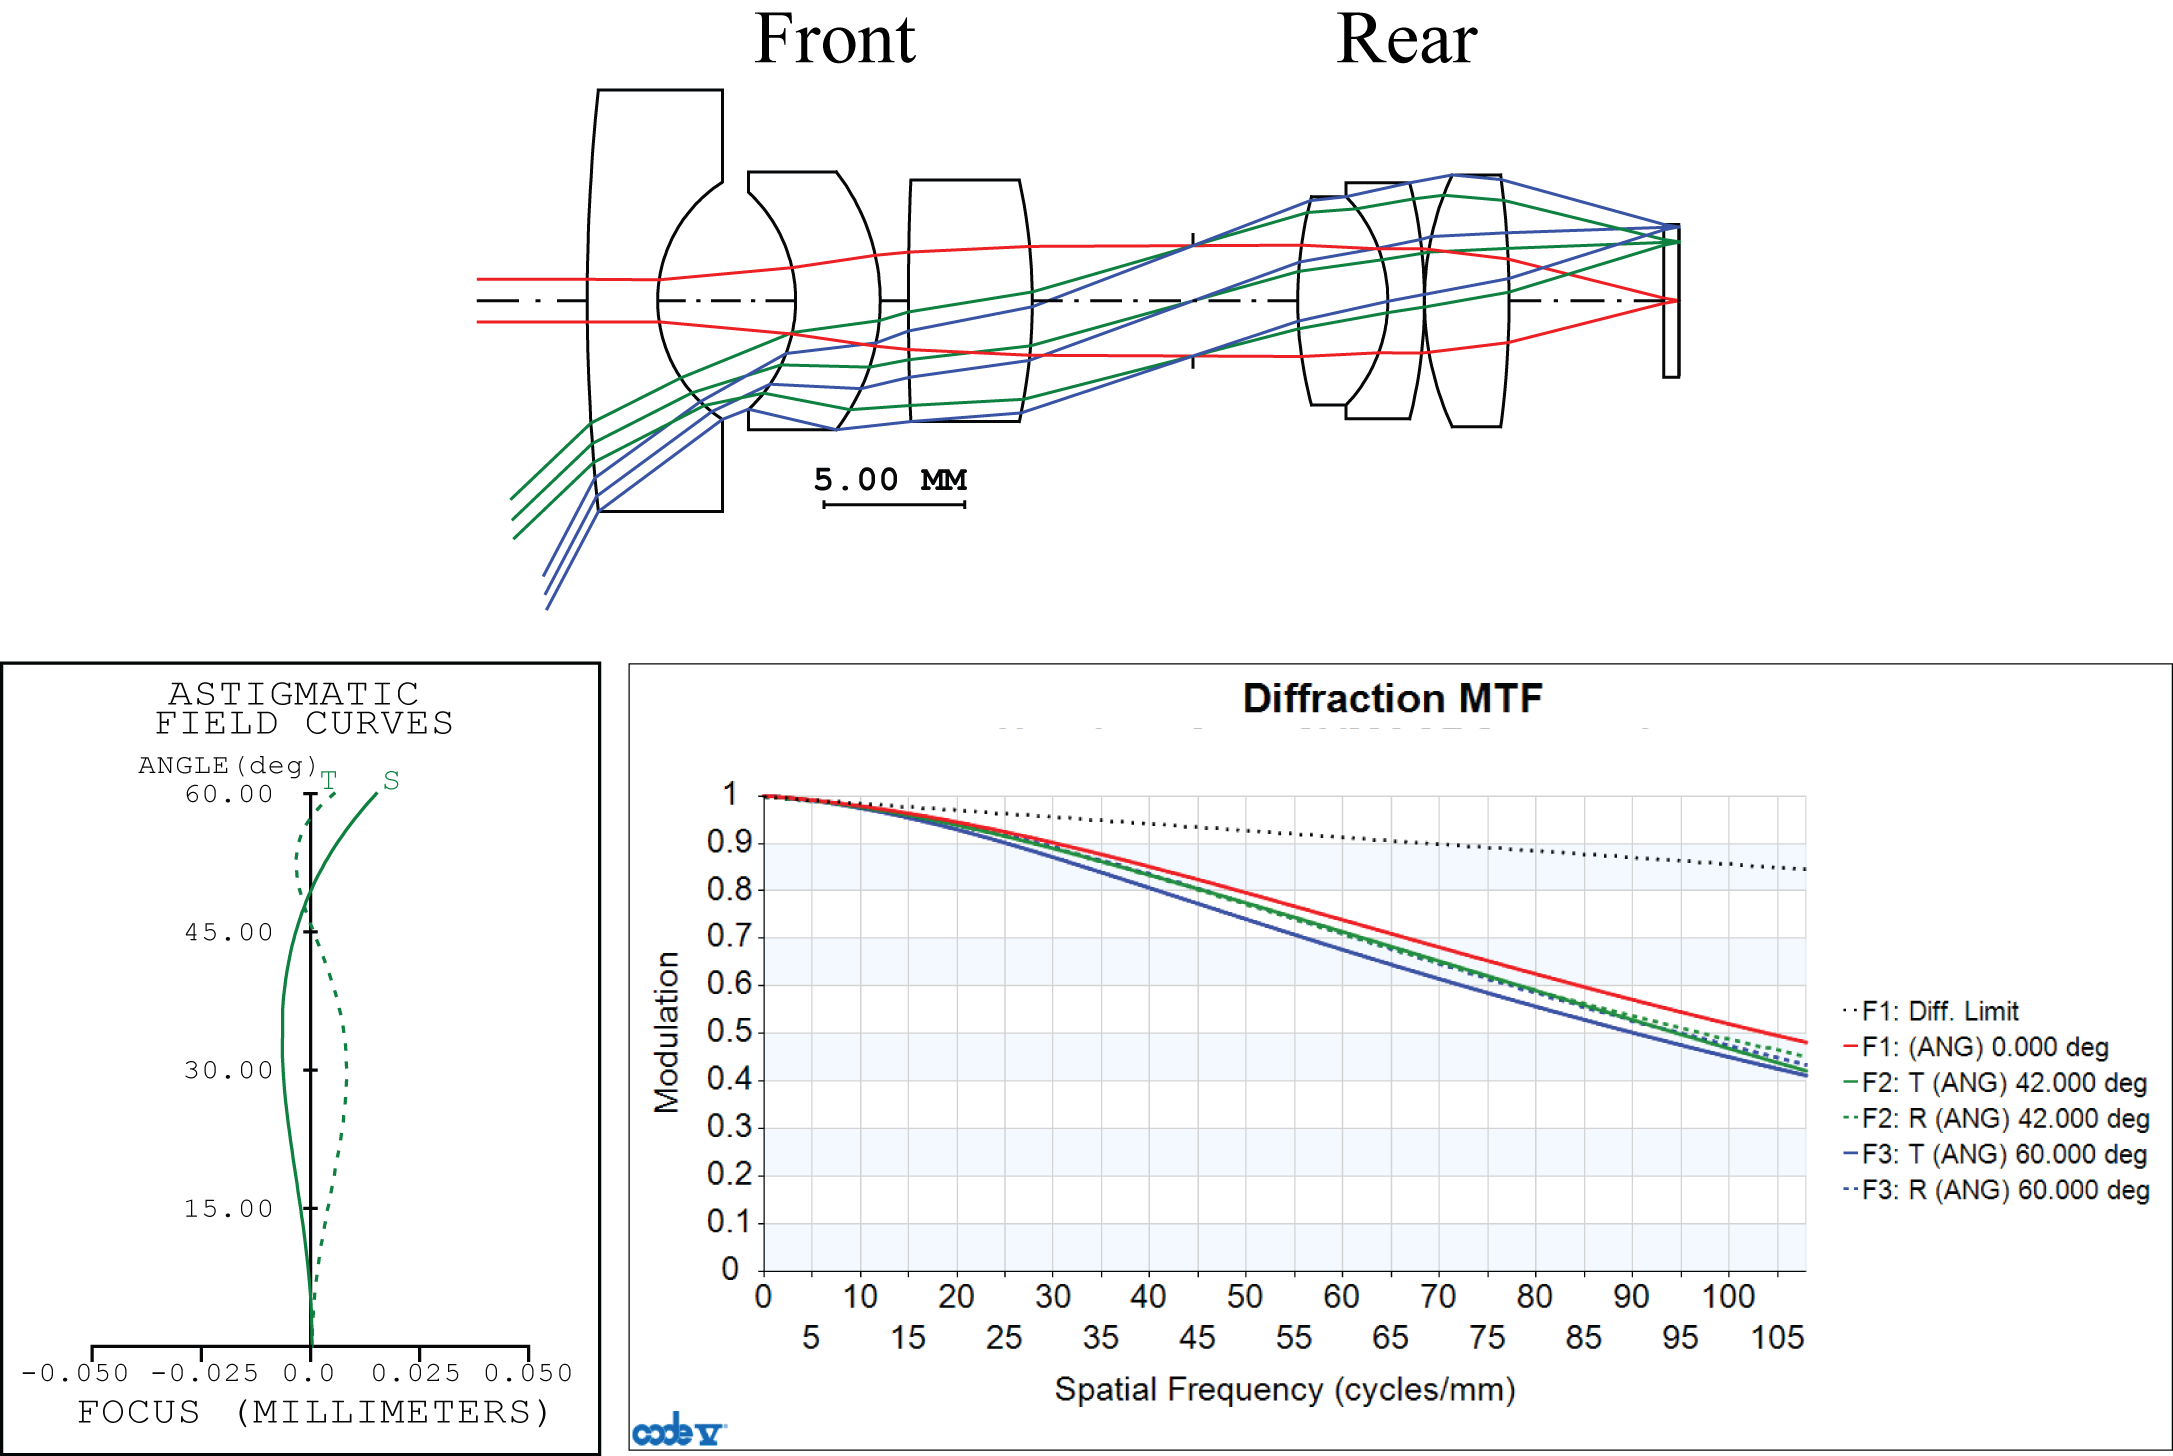
\includegraphics[scale=0.68]{chapter-4/figures/WideAngleL.png}
    \caption{System plot of a wide-angle lens and its performance.}
    \label{fig:wideanglelensPerformance}
\end{figure}

With the conventional method, the design of the front group started with a single lens using a flat and a concentric surface, given that the stop is at the right side of the lens. A moderate field of view is first used. Then lenses are added with either concentric or aplanatic surfaces. Adjustment and optimization are done to increase the field of view and achieve an angle reduction ratio of 0.3. The curvatures and thickness are both optimized. The rear group is designed separately by starting with a cemented flat surface doublet and two concentric surfaces. Another lens is added and a different glass is used to further reduce the monochromatic and chromatic aberration. The front group and rear group are then combined to optimize for the final solution.

When a solution is obtained by the conventional approach, SPC can be used to investigate alternative solutions. Since the system is combined from two separate parts, one way is to apply SPC to both the front and rear parts alone, without the other part being present. After that, different combinations of the front and rear parts can be investigated. Another way of applying SPC is to search for new solutions for the combined system.

After applying SPC to the front group and rear group alone, we obtain one solution for the front group and three solutions for the rear group. The next step is to combine the front group option with the rear group options. This is done by connecting the two groups and performing an optimization with the curvatures. All three cases provide the same final solution as illustrated in Figure \ref{fig:WAL_combine}.

\begin{figure}[h!]
    \centering
    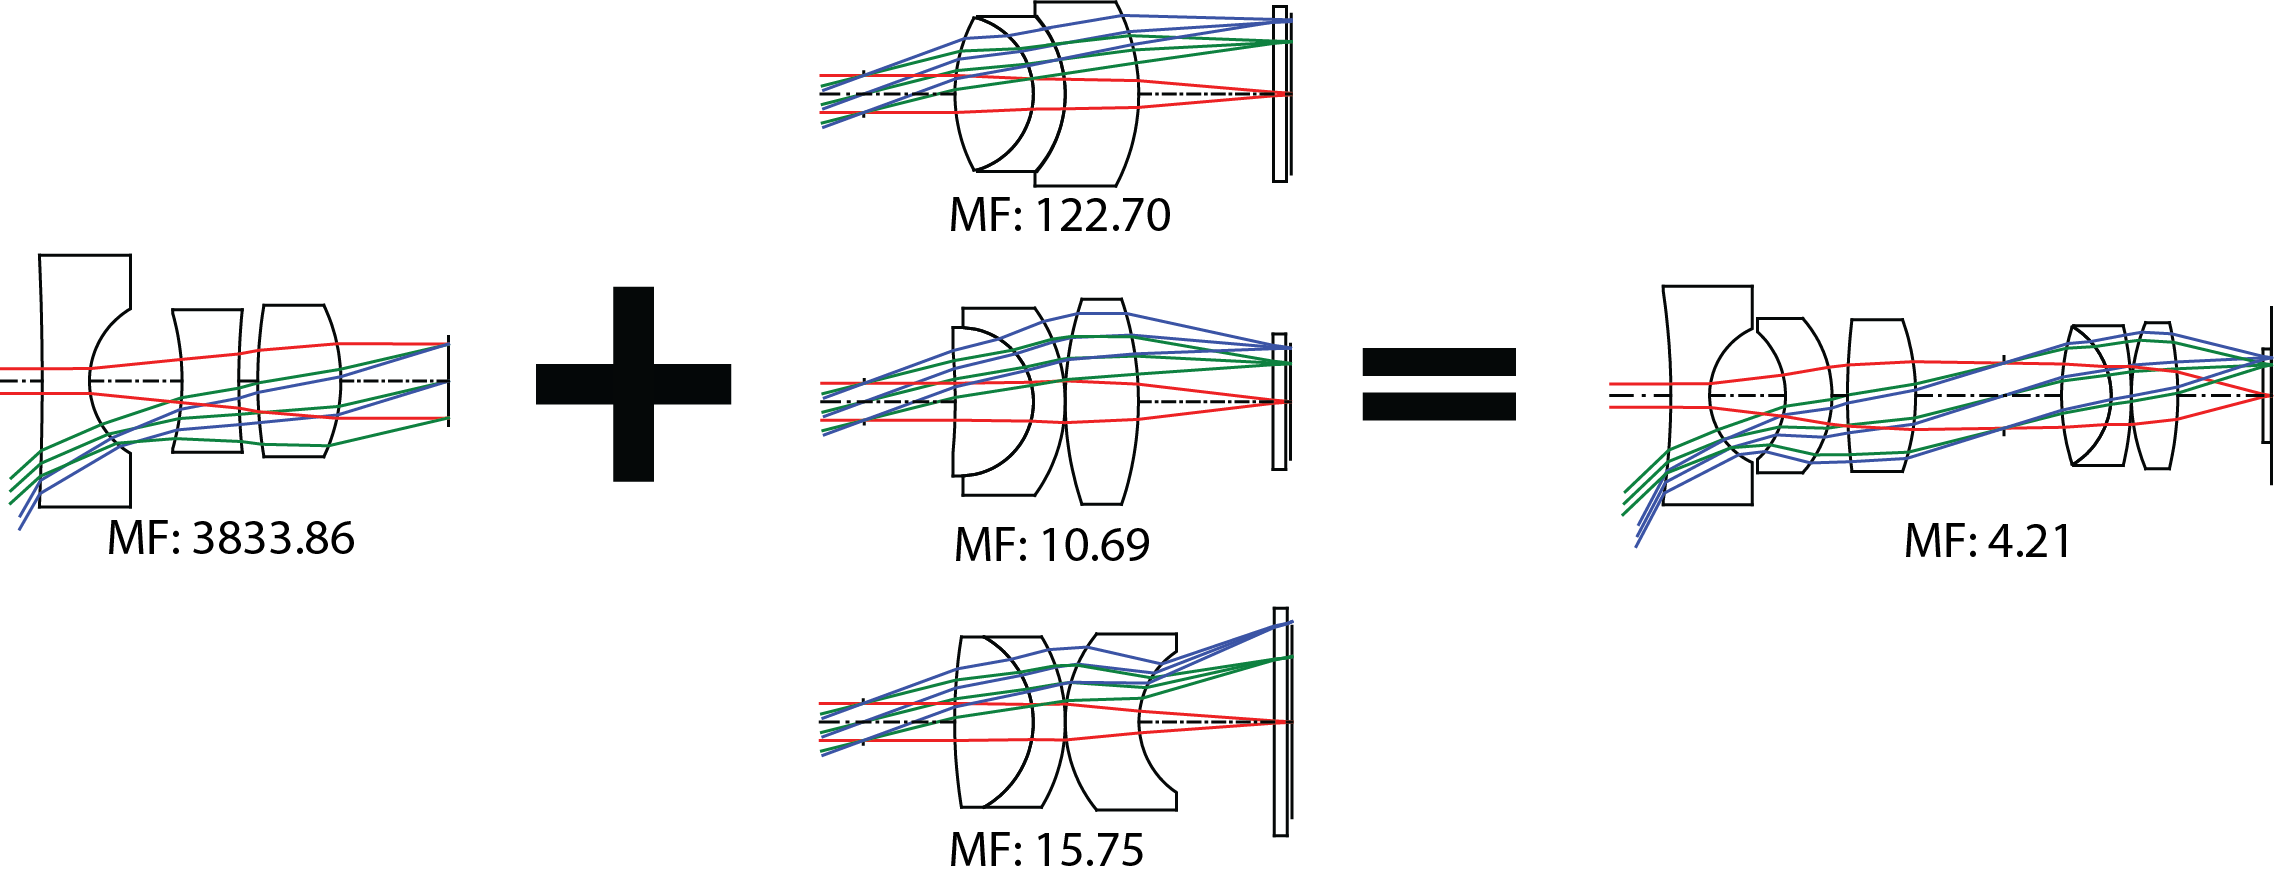
\includegraphics[width=0.7\textwidth]{chapter-4/figures/WAL_combine.png}
    \caption{Combinations of the front part (conventional approach) and the three rear parts (conventional with SPC). All converged to one solution. Merit Function (MF) values of the systems are provided. }
    \label{fig:WAL_combine}
\end{figure}

Once the combined system is obtained, SPC is performed to search for alternative solutions with the same amount of variables. As explained in Chapter 3, the first step is to extract lenses from the original system. Because the first lens is responsible for collecting the large angle rays, extracting it from the system while keeping the large field of view is not possible. The only possible lenses to extract and perform SPC scans are the second, third and last elements. The current SPC cannot be performed on cemented elements for switching to a different solution. It is because a cemented lens requires the two sub-elements to be in contact (having a shared surface). A null element cannot be created in such a situation while varying the curvatures for the SPC scan. The merit function based on transverse aberration in CODE V is used in this example. It is a composite value, scaled so that it is the mean square of the weighted image radius (unit: \textmu m$^2$). We keep the paraxial marginal ray exit angle as $-0.25$ rad on the last surface to ensure that the effective focal length is equivalent to $3.0$ mm (the entrance pupil diameter is 1.5 mm). Ten curvatures are used as variables. Six different minima are found in the design network illustrated in Figure \ref{fig:WAL_network}. A global optimization run (Global Synthesis of CODE V) is also performed. No additional local minima are found compared to the result of SPC. From Figure \ref{fig:WAL_network}, it is noticed that the major difference in the systems are in the front group. The system shape stays the same for the rear group in all six solutions.

The relationship between different systems is indicated by arrows in Figure \ref{fig:WAL_network}. Black arrows show that via SPC, two systems are connected in both ways. If M1 and M2 are connected in both ways, it means that by using SPC, M2 can be found starting from M1, and vice versa. Blue arrows indicate a one-way connection. For example, starting from M2, it is possible to find M3 via SPC. However, M3 does not lead to M2 by using SPC. Normally, the expected situation is a two-way connection. However, a one-way connection can appear in two scenarios: In the first scenario, a system with high stress and higher value of merit function is unstable (e.g. M6). The stability indicates the size of the basins of attraction. An unstable local minimum has a relative smaller basin of attraction compared to others. Therefore, it is easy to get out of this kind of poor local minimum with SPC. However, it is not easy (and not necessary for practical purposes) to reach them. The second scenario happens when two minima are very close to each other in the design space (e.g. M1 and M2). The landscape has relative smaller variation in this region around the two close minima. In Figure \ref{fig:WAL_network}, systems M1 and M2 (best two systems) have similar system shapes and close values of the merit function. Another system, such as M3 or M4, obtained by switching from M2, can easily, when switched back, go to M1. 

As shown in Figure \ref{fig:WAL_network}, all minima are connected within one network. It means that starting from any of the minima in the network, there is always a route to reach any other system. It can also be observed that the less good solutions (M3, M4, M5, and M6) are all directly connected with best two systems (M1 and M2). This implies that if the design process was trapped in one of the poor solutions, applying SPC once would be sufficient to switch to one of best two systems.  

\begin{figure}[h!]
    \centering
    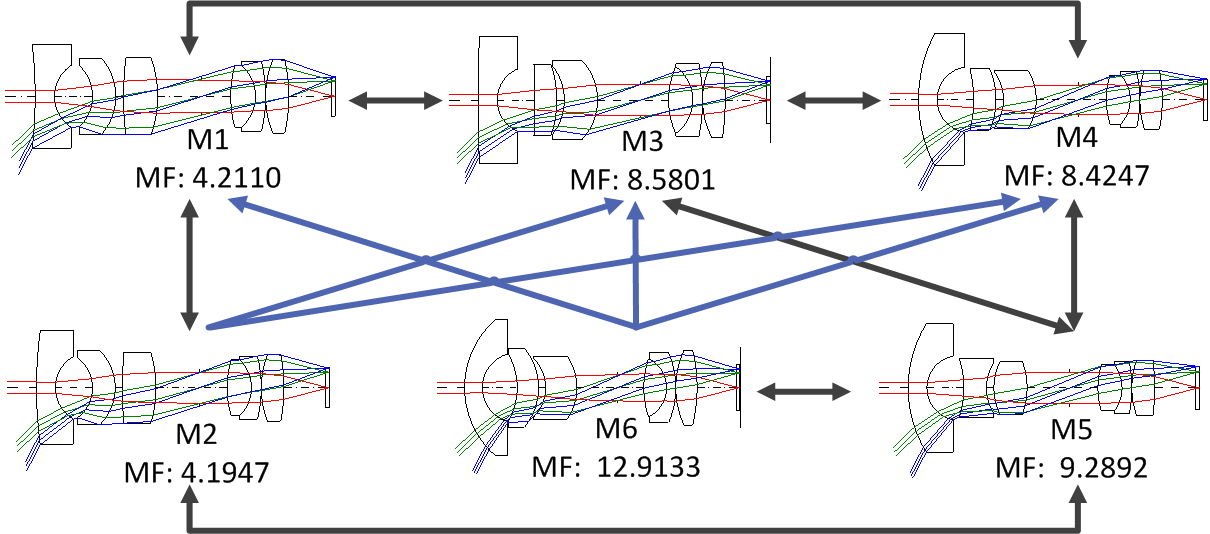
\includegraphics[width=0.8\textwidth]{chapter-4/figures/WAL_network.png}
    \caption{A network of minima for the wide-angle lens. All systems are connected with SPC. Global optimization using CODE V did not find additional systems. The transverse ray aberration in CODE V is used as the merit function.}
    \label{fig:WAL_network}
\end{figure}

\subsection{Stepwise Analysis of SPC for a Wide-angle System}
\subsubsection{Visualization of the Saddle Point }
In Chapter 3, recommendations have been given for applying SPC in steps. Examples are presented in this section to demonstrate how SPC is applied to the wide-angle system. The system M3 in Figure \ref{fig:WAL_network} is selected to demonstrate how SPC is practically performed. First, by extracting (details are described in Chapter \ref{cp2-switching}) the second element from M3, a minimum with one lens less is obtained. Then, a null element is inserted at the the same position where the lens is extracted and an SPC scan \ref{para: performing SPC scan} is performed on the null element. This null element is not in contact with the existing lens elements in front of or behind it.  With the SPC scan, curvatures of the null-element are chosen such that saddle point systems are obtained. Figure \ref{fig:WAL_demo_sp} shows the SPC scan curve (Figure \ref{fig:WAL_demo_sp}(b)) and the corresponding saddle point system (Figure \ref{fig:WAL_demo_sp}(a)) which is found by the scan. In an SPC scan curve, the crossing of the curve and the horizontal axis indicates the curvature of the saddle point system (the black dot in Figure \ref{fig:WAL_demo_sp}(b)). In this case, only one saddle point system is found via the scan and the curvature of the saddle point system is -0.170 $mm^{-1}$. 

The saddle point system obtained using SPC scan is usually a saddle point with a Morse Index of 1. This means that there exists a 2D plane in the high-dimensional design space where from the obtained saddle point, along one direction the value of merit function decreases, and along another (orthogonal to the previous one) the value increases. Given this 2D plane, the saddle point can be be visualized (Figure \ref{fig:WAL_demo_sp}(c)). 
\begin{figure}[h!]
    \centering
    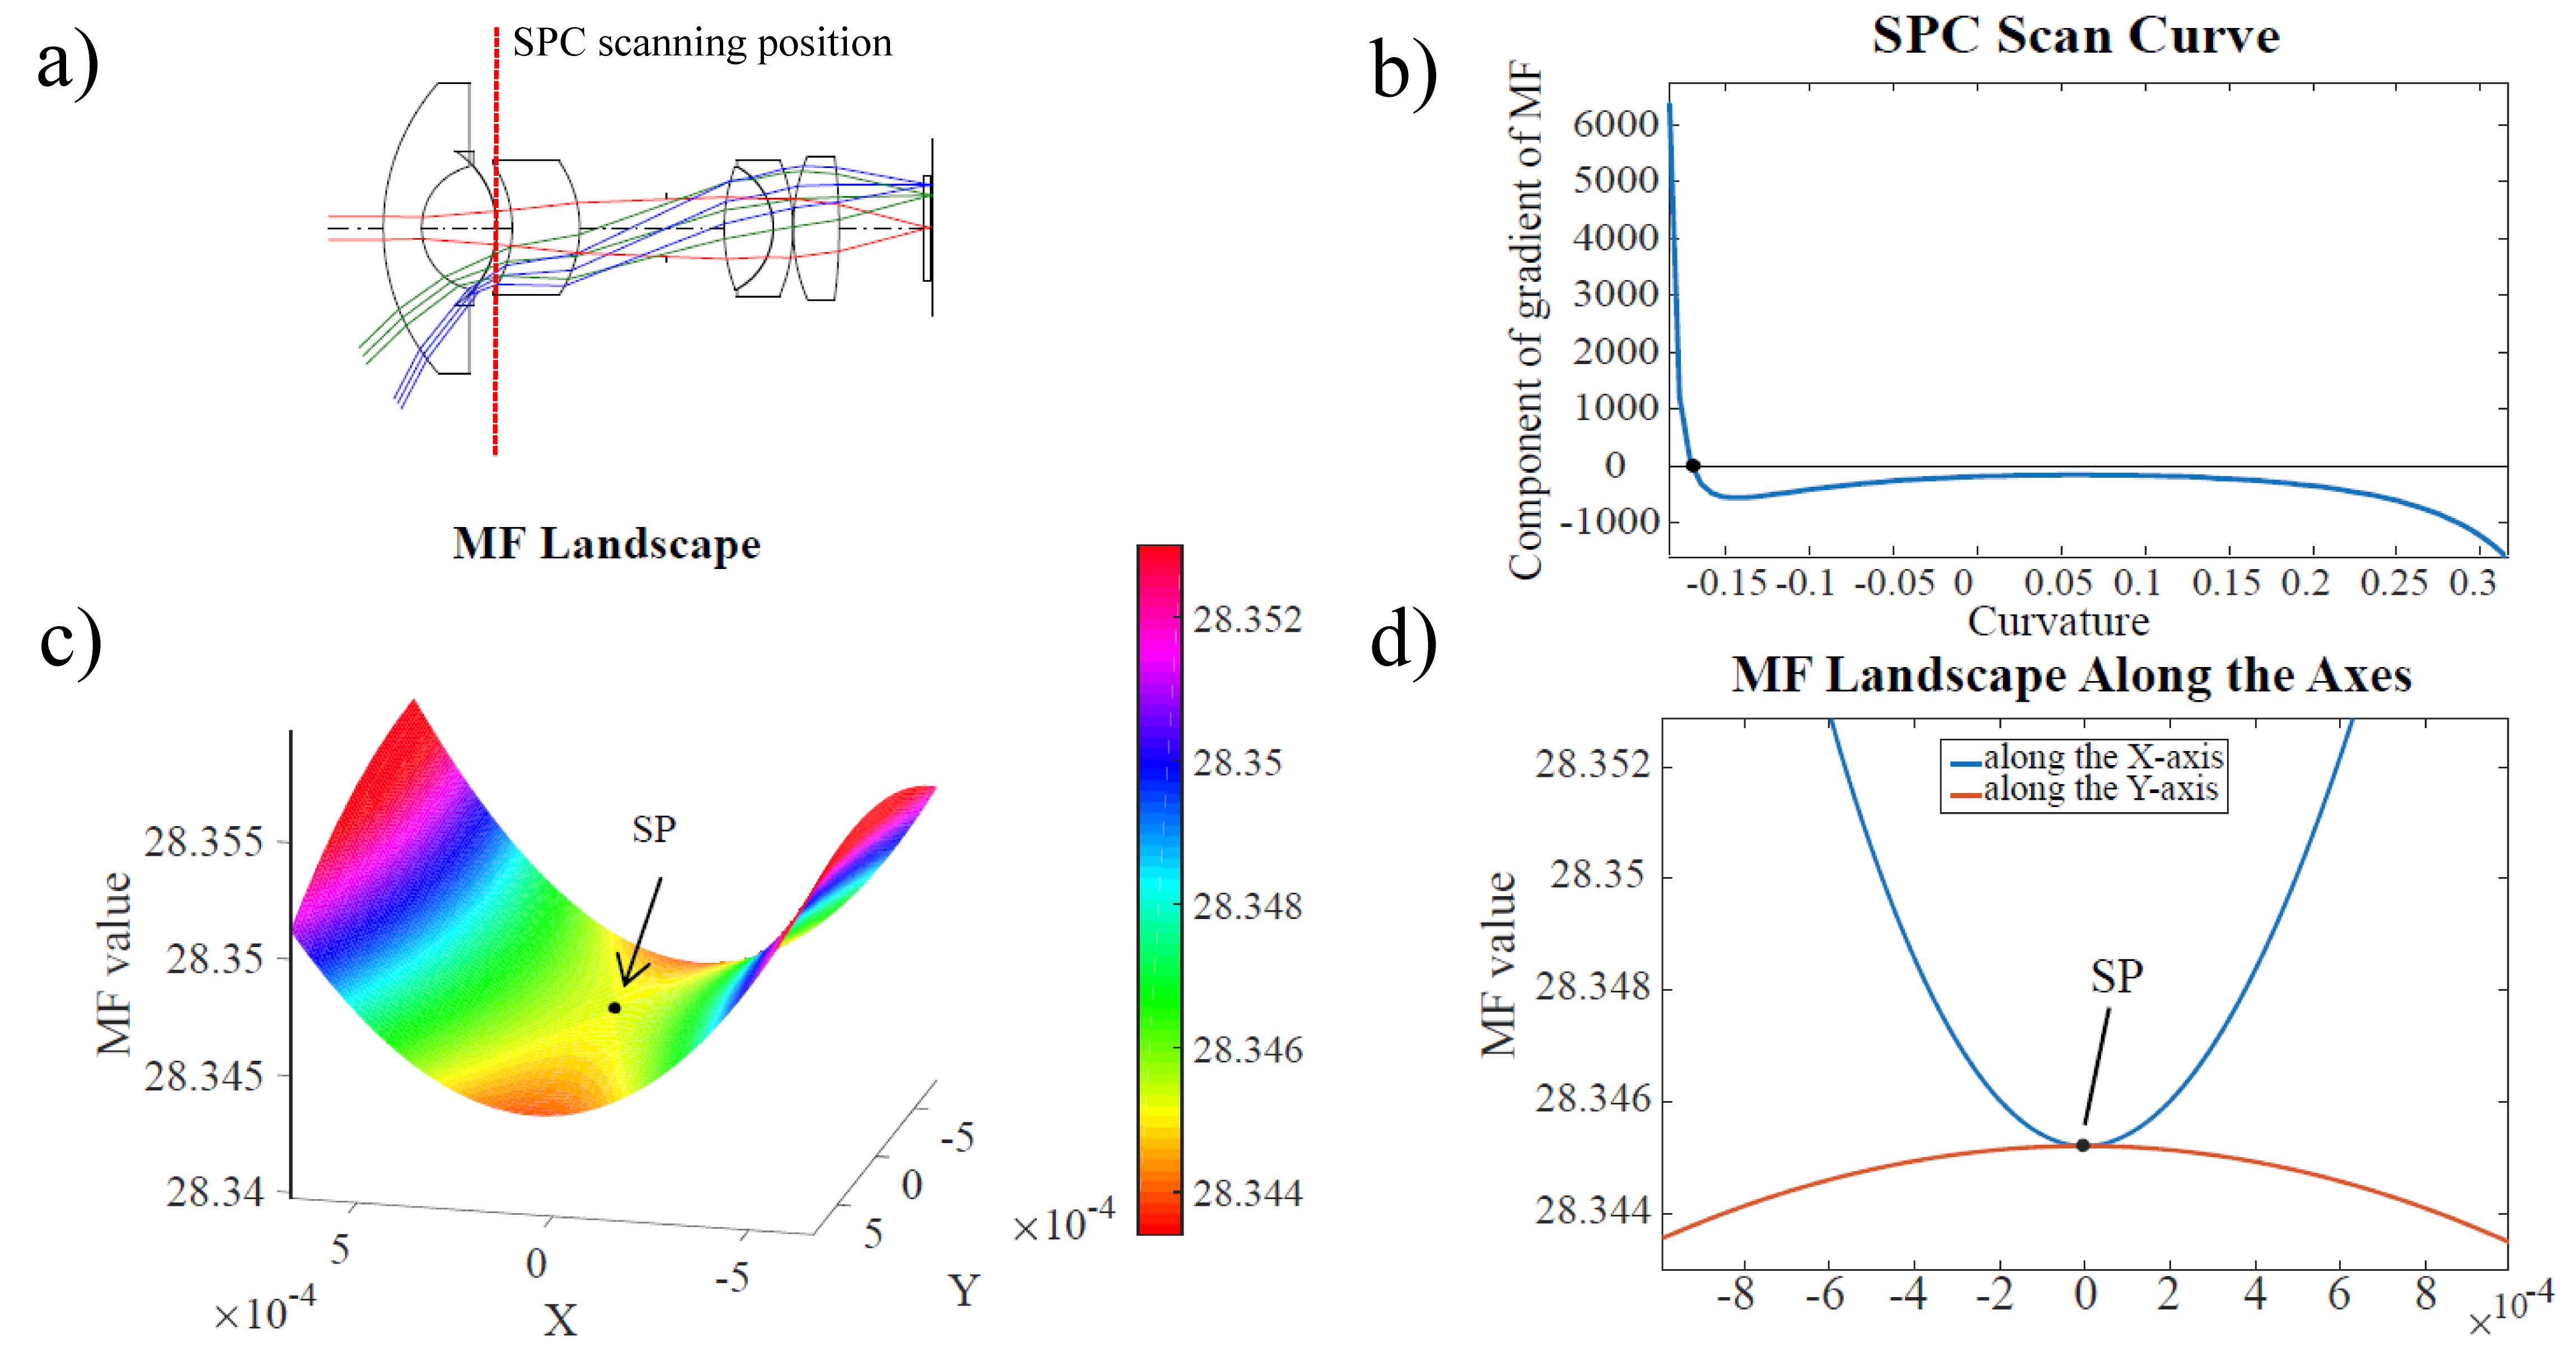
\includegraphics[width=\textwidth]{chapter-4/figures/WAL_demo_sp.png}
    \caption{a): the system we choose for the SPC scan. b): the SPC scan curve. c): the saddle point visualized in the chosen 2D plane (Figure \ref{fig:hyperplane}. d): the descending and ascending direction around the saddle point in the same 2D plane. The saddle point is marked with a black dot.}
    \label{fig:WAL_demo_sp}
\end{figure}

The value of the merit function for the saddle point equals the value of the merit function at the minimum before adding the extra two variables. If the direction where the merit function decreases can be determined, then the 2D plane to visualize the saddle point can be easily chosen. Numerically, this direction can be determined by minimizing on a hyperplane, which is orthogonal to the SPC scan line along which the merit function value is constant. In Figure \ref{fig:hyperplane}(a), we use a 3D case to demonstrate how such a hyperplane is found. The 3D space has the coordinates $(x_1, \eta, \xi)$. The variables are explained in Figure \ref{fig:hyperplane}(b): $x_1 = c_1$, where $c_1$ is the curvature variable which does not belong to the null element; $\eta = c_2 + c_3$, $\xi = c_2 - c_3$, where $c_2$ and $c_3$ are the curvatures of the null element.  Point $S (x_{1,m}, \eta_{s}, 0)$ is the saddle point system containing the null element. Point $A$ is a point on the line close to Point $S$ where the merit function value is constant. And the value of the merit function is the same as Point $S$. An example of the merit function landscape in the $x_1, \eta$ plane is given in Figure \ref{fig:hyperplane}(c). Along the line $SA$, the value of the merit function is constant, hence, to find the direction of descent in a $N$-dimensional space, we have to move in the $(N-1)$-dimensional hyperplane which is perpendicular to the line $SA$. It is the 2D plane $P1$ as shown in Figure \ref{fig:hyperplane}(a). On this plane, $B$ is a point where the merit function value is minimized. We will have $MF_{B}$ < $MF_{S}$. With points $A$, $B$ and $S$, a 2D plane $P2$ can be determined in which we can plot both the directions of ascent and descent . Given the two vectors on the 2D plane, $\overrightarrow{SA}$ and $\overrightarrow{SB}$, an orthogonal base can be calculated with the Gram-Schmidt process:

\setlength{\belowdisplayshortskip}{5pt}
\setlength{\abovedisplayshortskip}{5pt}
\begin{equation} \label{eq:u1}
\pmb{\beta_{1}} =  \left\| \overrightarrow{SA}-{\frac{\langle \overrightarrow{SA},\overrightarrow{SB}\rangle}{\langle \overrightarrow{SB},\overrightarrow{SB}\rangle}}\overrightarrow{SB} \right\|,  \; \; \; \hat{u}_{1} = \frac{\pmb{\beta_{1}}}{\left\|\ \pmb{\beta_{1}}\right\|}
\end{equation}
\setlength{\belowdisplayshortskip}{10pt}
\begin{equation} \label{eq:u2}
\pmb{\beta_{2}} = \overrightarrow{SB}, \;\; 
\hat{u}_{2} =\frac{\pmb{\beta_{2}}}{\left\|\ \pmb{\beta_{2}}\right\|} ,
\end{equation}
 $\hat{u}_{1}$ and $\hat{u}_{2}$  are the two orthogonal unit vectors of the 2D plane. The 2D plane with the visualized saddle point can be plotted as shown in Figure \ref{fig:WAL_demo_sp}(c).

The system T2-M1 and T2-M4 in Table \ref{table: scanline} are situated in different basins of attraction (\ref{label: basinOfattrac}).  

\begin{figure}[h!]
    \centering
    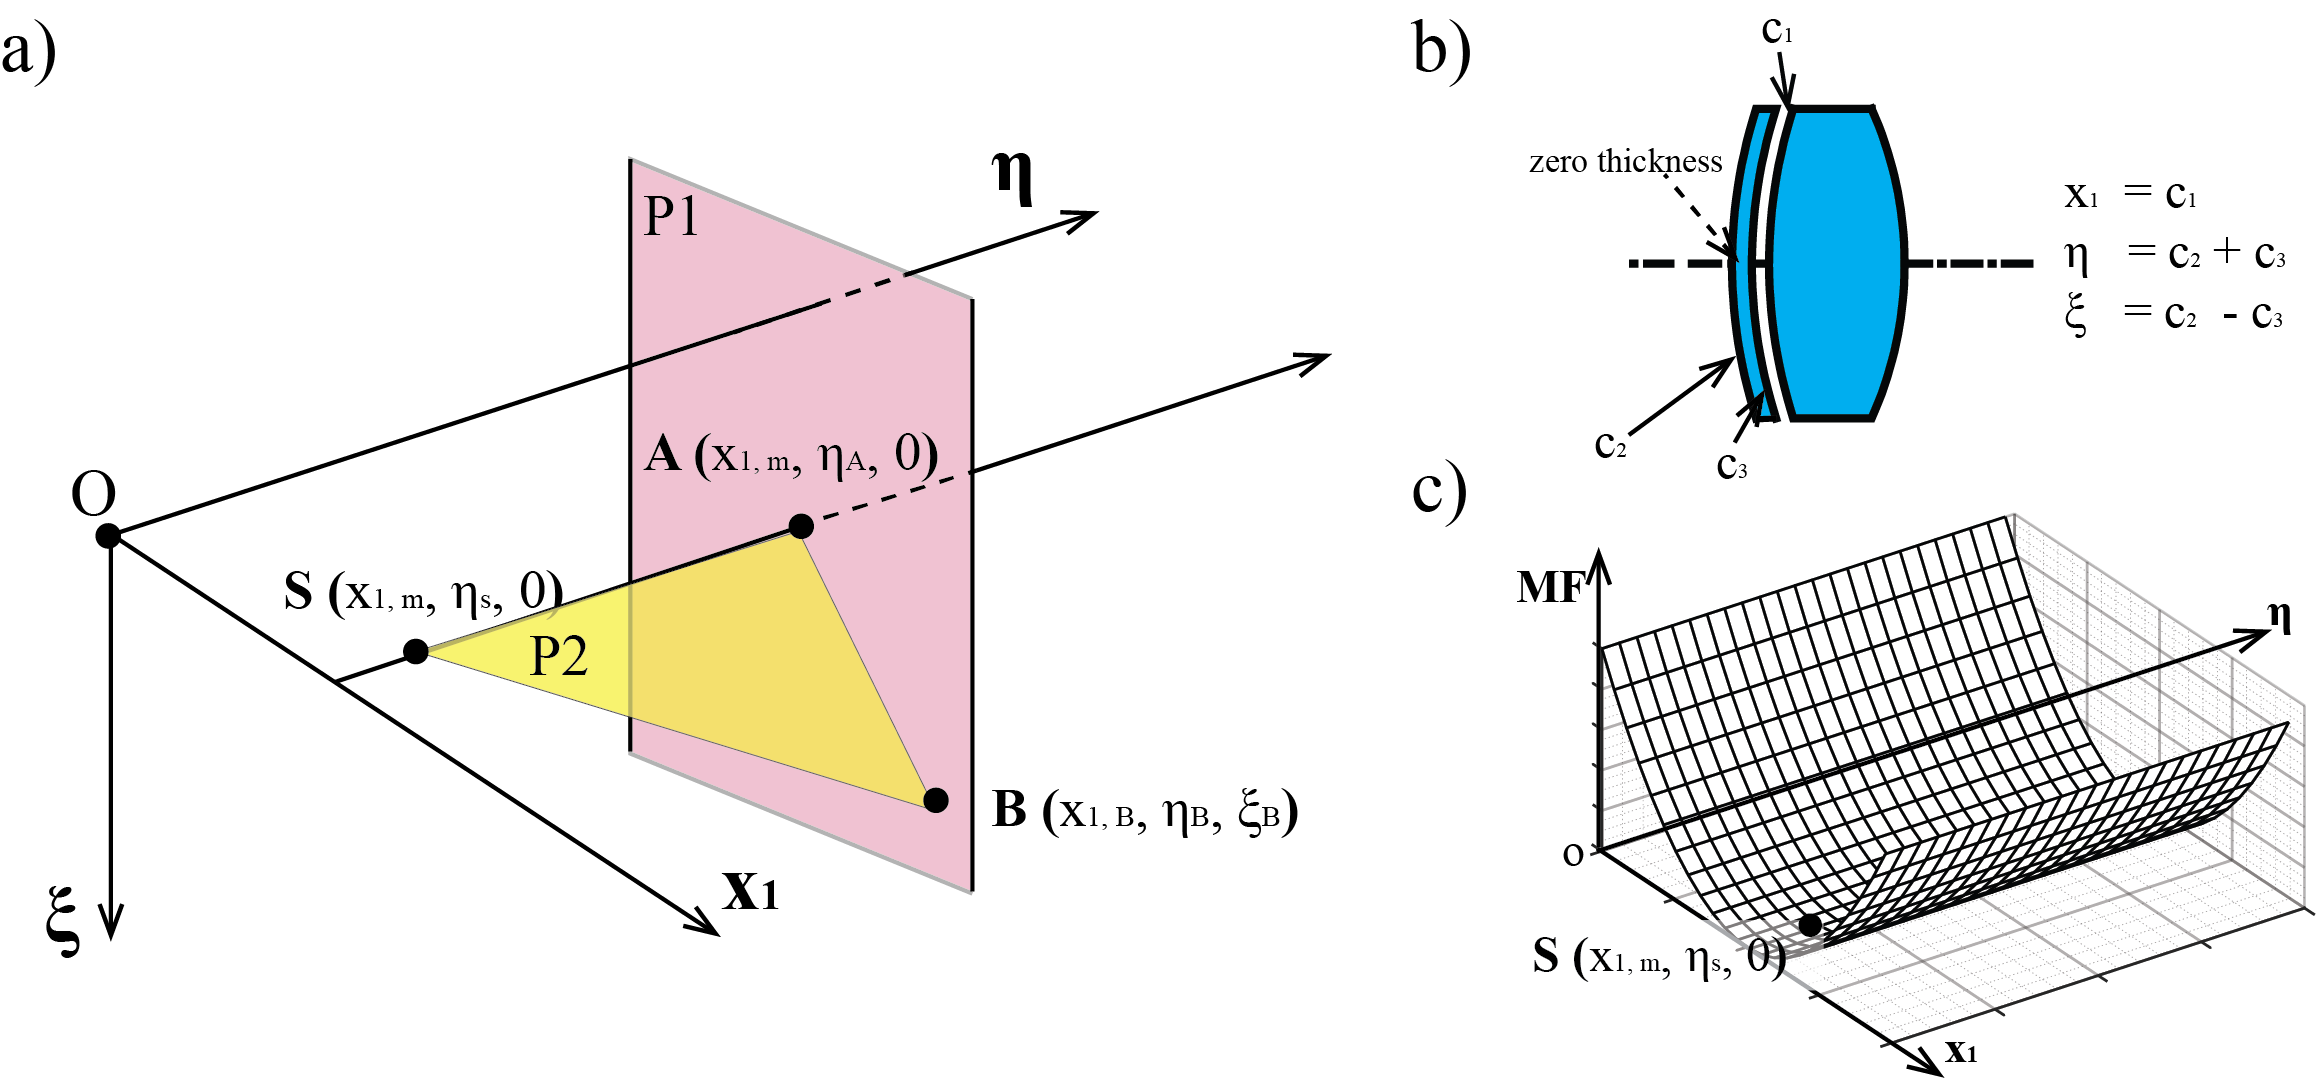
\includegraphics[width=0.985\textwidth]{chapter-4/figures/hyperplane.png}
    \caption{ a) The construction of a 2D plane P2 to visualize the saddle point S in a 3D dimensional example. Point A is a point on the SPC scan line. P1 is a hyperplane perpendicular to line SA. Point B is where the merit function value is minimized on P1. b) Explanation about variables and coordinates. When $\xi = 0$, the $x_1, \eta$ plane includes all the null element systems. c) Example of a merit function landscape in the $x_1, \eta$  plane. $x_{1, m}$ indicates the original minimum values before insertion of the null element.}
    \label{fig:hyperplane}
\end{figure}
In Figure \ref{fig:WAL_demo_sp}(d), the plots along the X and the Y direction show that the value of the merit function is increasing in one direction and decreasing in the other direction. Optimization routes following the descending directions on both sides of the saddle (on the Y-axis shown in Figure \ref{fig:WAL_demo_sp}(d)) lead to two distinct local minima.

\subsubsection{Choices of Starting Point of Local Optimization near the Saddle Point}
Visualizing a saddle point in the 2D plane $P2$ is good for demonstration and helps to choose the optimization direction, however, in practice, it is computationally expensive to look for the 2D plane for each saddle point. As mentioned previously, a common practice is to change the system along the SPC scan line, which means changing the curvatures of the inserted null-element with a small positive and negative value (this value is chosen empirically). The modified systems are the starting points for optimization. The optimization includes two curvature variables in addition to the variables where the minimum (without the null element) is obtained. In the experiment, choosing different values for the curvature change may lead to different minima. This is demonstrated in Figure \ref{fig: scanning_line}, where different values were chosen for the null-element curvature as a starting point to find  the corresponding local minimum. In order to better illustrate the phenomenon, the scan range chosen here (from -0.2 to 0.2) was larger than the curvature changes normally used in practice. From Figure \ref{fig: scanning_line}, it is observed that four different minima were obtained with different values chosen as the starting curvature. The corresponding system shapes and merit function values are shown in Table \ref{table: scanline}. 
\begin{table}[h!]
    \centering
    \captionsetup{justification=centering}
    \caption{Result of the optimization along the scan line (dashed boxes mark the zero-thickness elements).}
    \label{table: scanline}
    \vspace{-1em}
    \hspace*{-16.5pt} %adjusting the position of the plot(table)
    \begin{tabular}{l}
    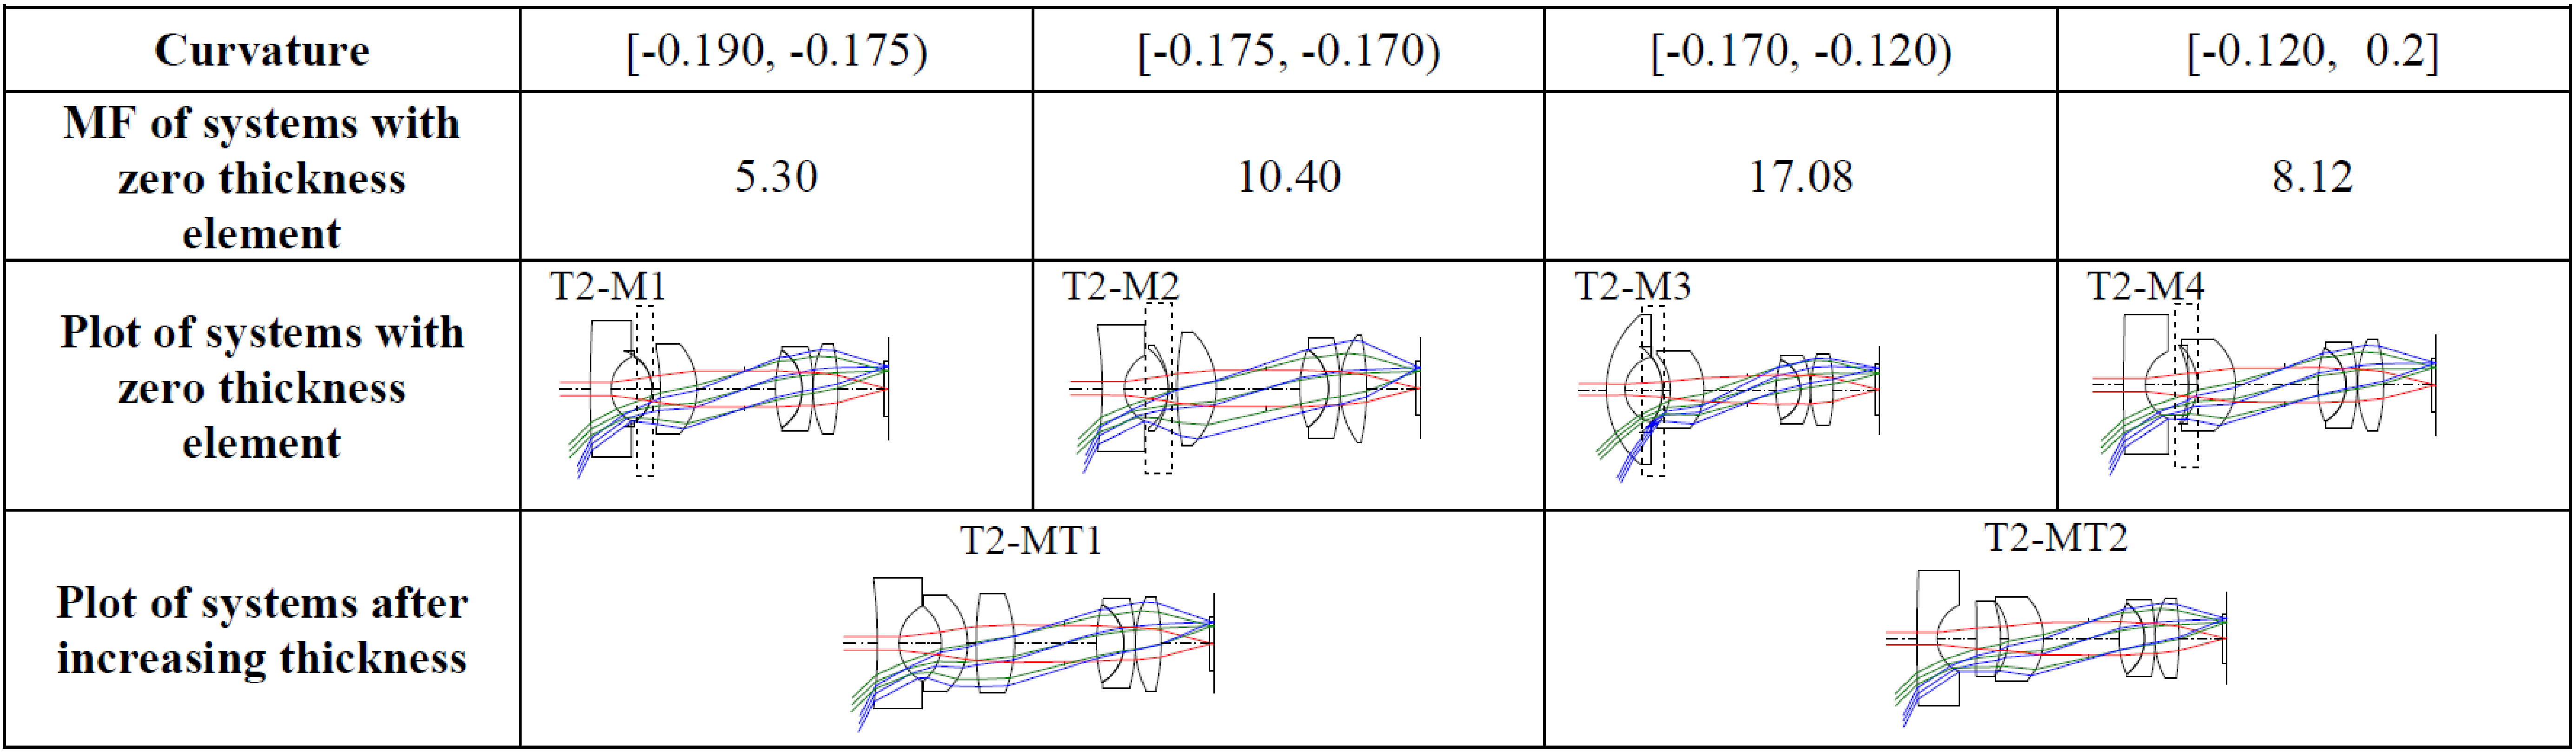
\includegraphics[width=0.98\textwidth]{chapter-4/figures/Line_Opt_table.png}
    \end{tabular}
\end{table}
\begin{figure}[h!]
    \centering
    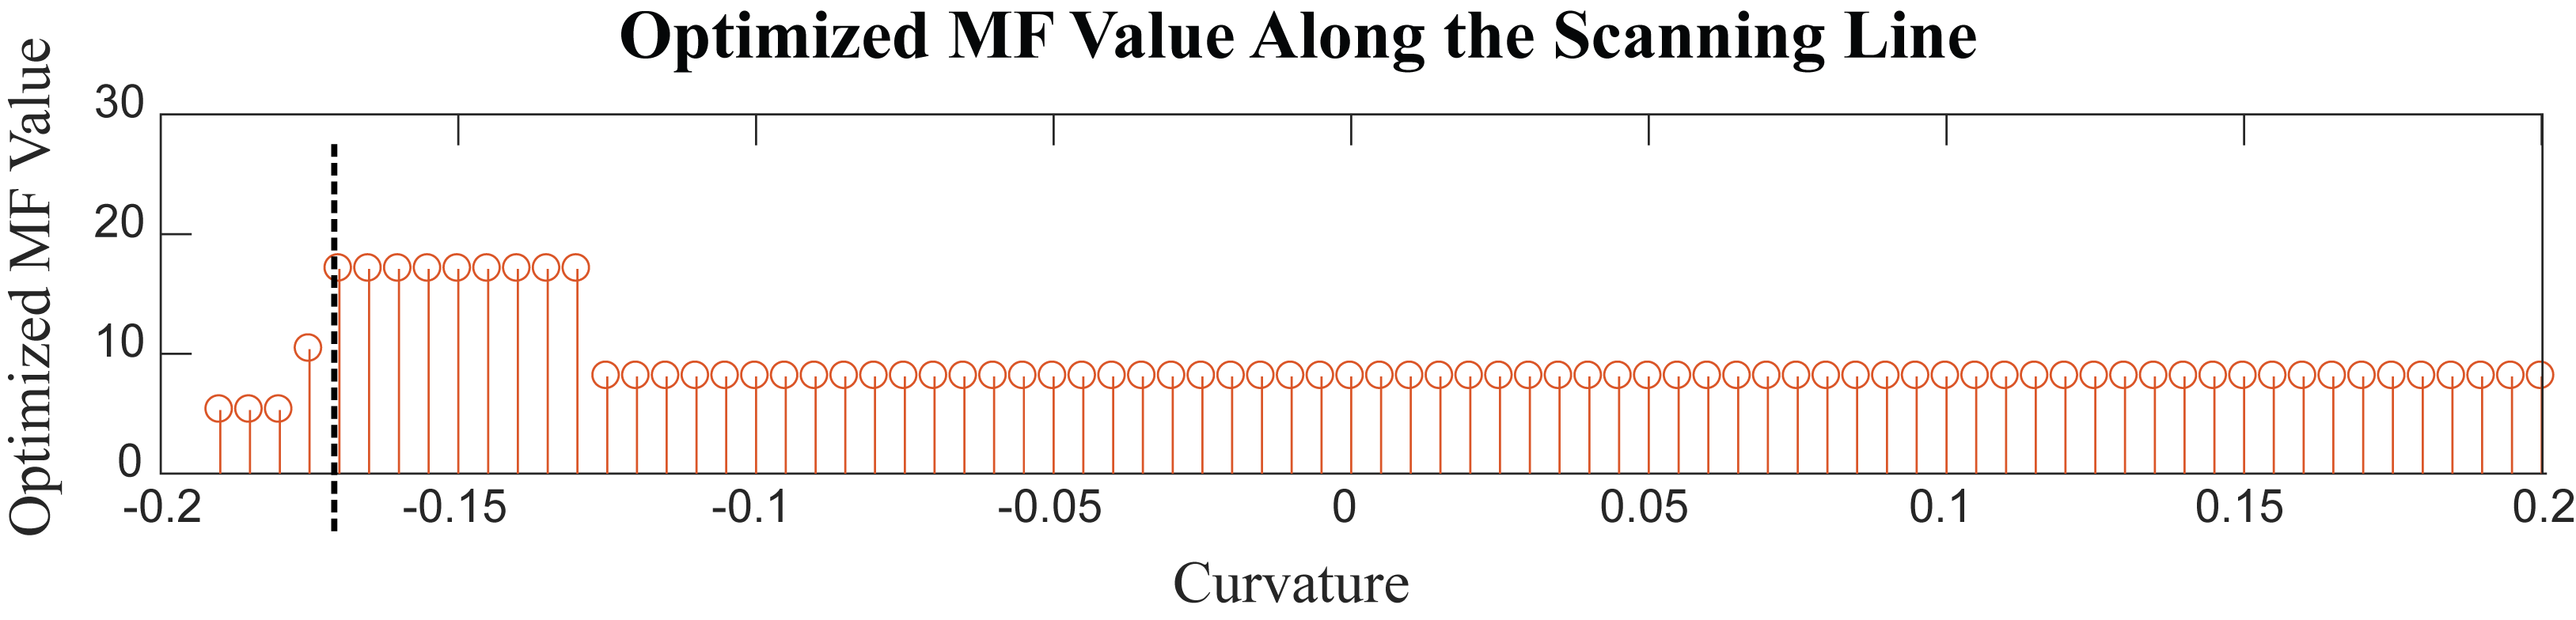
\includegraphics[width=0.95\textwidth]{chapter-4/figures/Scanning_Line_plot.png}
    \caption{Optimized MF value along the scan line. The vertical dashed line indicates the saddle point curvature. The stepsize is 0.05.}
    \label{fig: scanning_line}
\end{figure}

In Figure \ref{fig: scanning_line}, with a curvature step size of 0.05, we see that different local minima are obtained around the curvature value of the saddle point. It indicates that near the saddle point, the local optimization is still sensitive to the choice of the starting point. To better understand the basin of attractions near the saddle point, we have also investigated the cases where the starting point is selected on a 2D plane instead of the one-dimensional scanning line. The constructed saddle point is located in this 2D plane. We have used two different approaches to determine such 2D planes. The first method is to find the plane defined by Equation \ref{eq:u1} and \ref{eq:u2}. On this plane, the saddle point can be visualized and in principle selecting starting points on the opposite side of the saddle point leads to two different local minima. The second method is to construct a plane directly using the two newly inserted variables (two curvatures of the null element). The first method serves as the reference since it clearly captures the ascending and descending directions around the saddle point. However, computing such a plane needs additional effort. The second method is a computation-wise simple way. By comparing the two, we would like to study if a simple approach is sufficient to obtain reliable starting points around the saddle point. 

As shown in Figure \ref{fig:basins}, the plot of the optimization results can also be called the plot of the basins of attraction. The same colour indicates that all starting points from that region (basin) end in the same local minimum after local optimization. The left side of Figure \ref{fig:basins} shows the basins of attraction in a relatively large region, from which the complexity of the optimization landscape can be observed. On the right side of the plot, the region around the saddle point is shown enlarged. In both plots, the scan line divides the basins into two parts: the green part converging to the minimum with a merit function value of 8.12 (T2-M4 in Table \ref{table: scanline}) and the red part converging to the minimum with a merit function value of 5.30 (T2-M1 in Table \ref{table: scanline}). In both cases, we also observe that if the starting points are chosen on the scan line, the optimization may converge to the minimum with a merit function value of 17.08 (yellow color) or the minimum with a merit function value of 10.40 (navy blue color). The red and green regions represent the two basins on both sides of the saddle point. However, in this case, choosing starting points on the scan line may lead to unwanted local minima. Practically, it is still recommended to choose the starting points on the 2D plane defined by the two inserted variables since constructing the hyperplane needs additional steps of constrained optimization. From the plots in Figure \ref{fig:basins}, it is evident that a better way to choose the starting points is to avoid the scan line, for example, by choosing a point on a line that is perpendicular to the scan line. It is also seen that the starting points should not be too far away from the saddle point. Otherwise, the two basins around the saddle point will be missed. In Figure \ref{fig:basins}(b), the saddle point has coordinates $(-0.1702,-0.1702)$. The closest starting point where the optimization converges to an unwanted minimum is $(-0.1713, -0.1675)$. The distance between this starting point and the SP is $0.0029$, which is $1.7\%$ of the absolute value of the curvature at the saddle point. It indicates in this example that even with a small step, optimization can go to a local minimum which is not expected. Practically, it suggests that more than two starting points around the saddle point are needed such that the minima connected to this saddle point is obtained. 

\begin{figure}[h!]
    \centering
    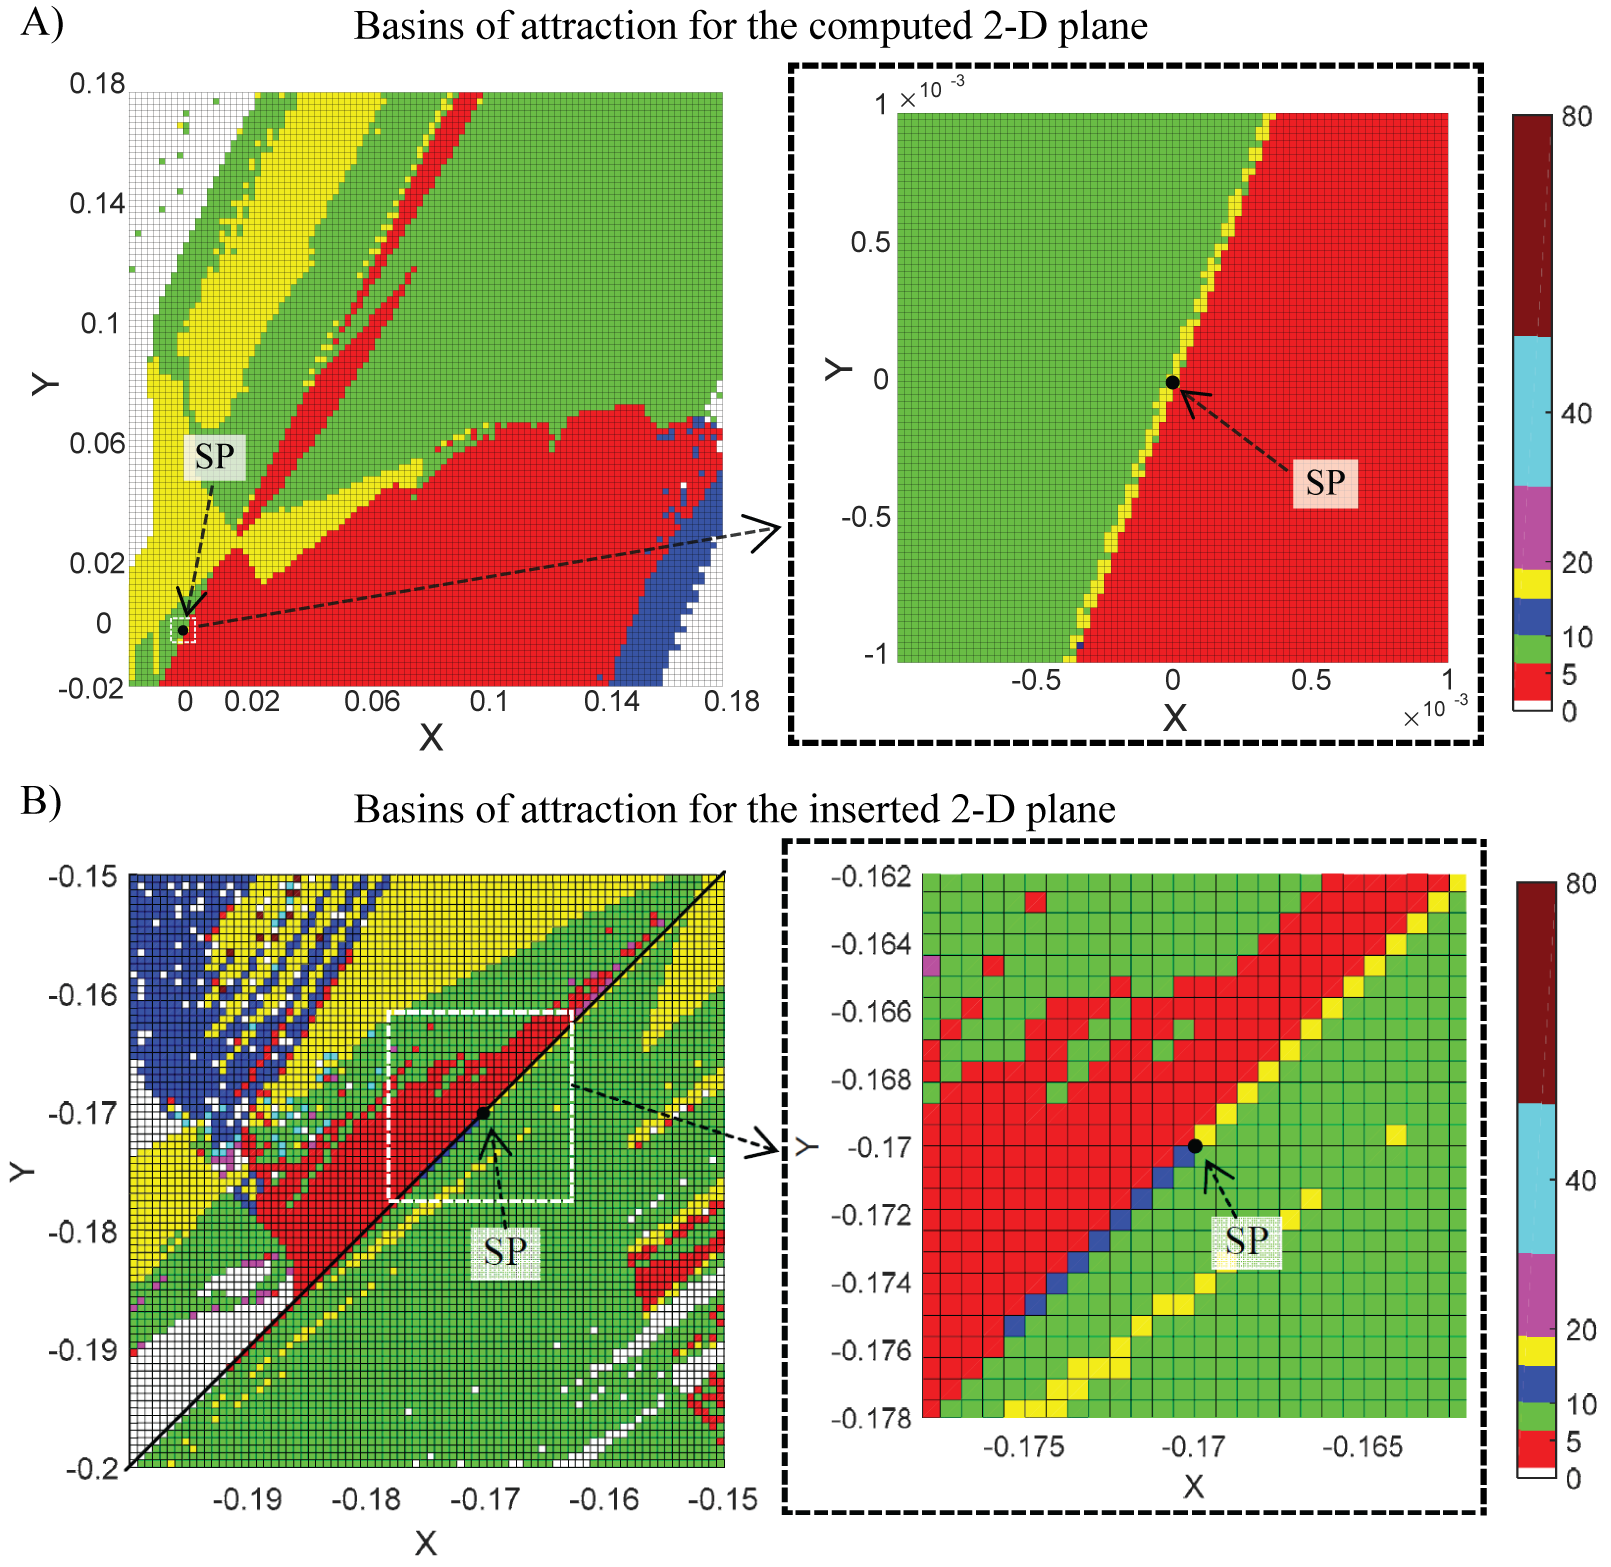
\includegraphics[width=0.8\textwidth]{chapter-4/figures/Basins_two_situations.png}
    \caption{Basins of attraction around the saddle point in 2D planes. a) Computed 2D plane where x and y are the variables defined by equation \ref{eq:u1} and \ref{eq:u2}; b) 2D plane given by the two newly inserted variables. The saddle points (SP) are marked by black dots.}
    \label{fig:basins}
\end{figure}

It is not clear in the presented example why on the scan line the optimization might lead to other solutions than the expected ones. It has been demonstrated in previous research done by van Turnhout \cite{vanTurnhoutThesis2009} (Page 81)\cite{vanTurnhout2009_landscape_instab} that when the damping factor of the damped least square algorithm is sufficiently large, there will be less artefacts shown in the plot of the basins of attraction. A hypothesis is that on the scan line there will also be no artefact locations that cause convergence to a different local minimum. In the example presented here, there is no control over the damping factor because the local optimizer of CODE V is used, hence, it is not possible to identify the cause of the behaviour along the scan line. 

It follows that by using a different position for the extraction of a lens and subsequently applying SPC, it is found in Figure \ref{fig:basins_WAL_M3_S5} that a different behaviour occurs along the scan line. In this case, the third lens element was extracted. As shown in Figure \ref{fig:basins_WAL_M3_S5}, along the scan line there are no starting points that lead to different local minima other than the expected two. Local optimization will either converge into a local minimum in the green region with merit function value MF = 44.53, or to a local minimum in the orange region with MF = 37.82. The white region (MF = 0) indicates ray failure. The furthest starting point with respect to the saddle point, at which the system can still be ray-traced, is at $(-0.1893, -0.1960)$. The coordinates of the saddle point are $(-0.1903, -0.1903)$. The distance between the saddle point and this starting point is $0.0058$, which is $3.0\%$ of the absolute value of the curvature of the saddle point. This is a small distance. It again indicates in this example that optimization can become unstable if the starting points around the saddle points are not chosen properly. Similar to the previous example, it suggests that in practice, more starting points around the saddle points should be selected. 
\begin{figure}[h!]
    \centering
    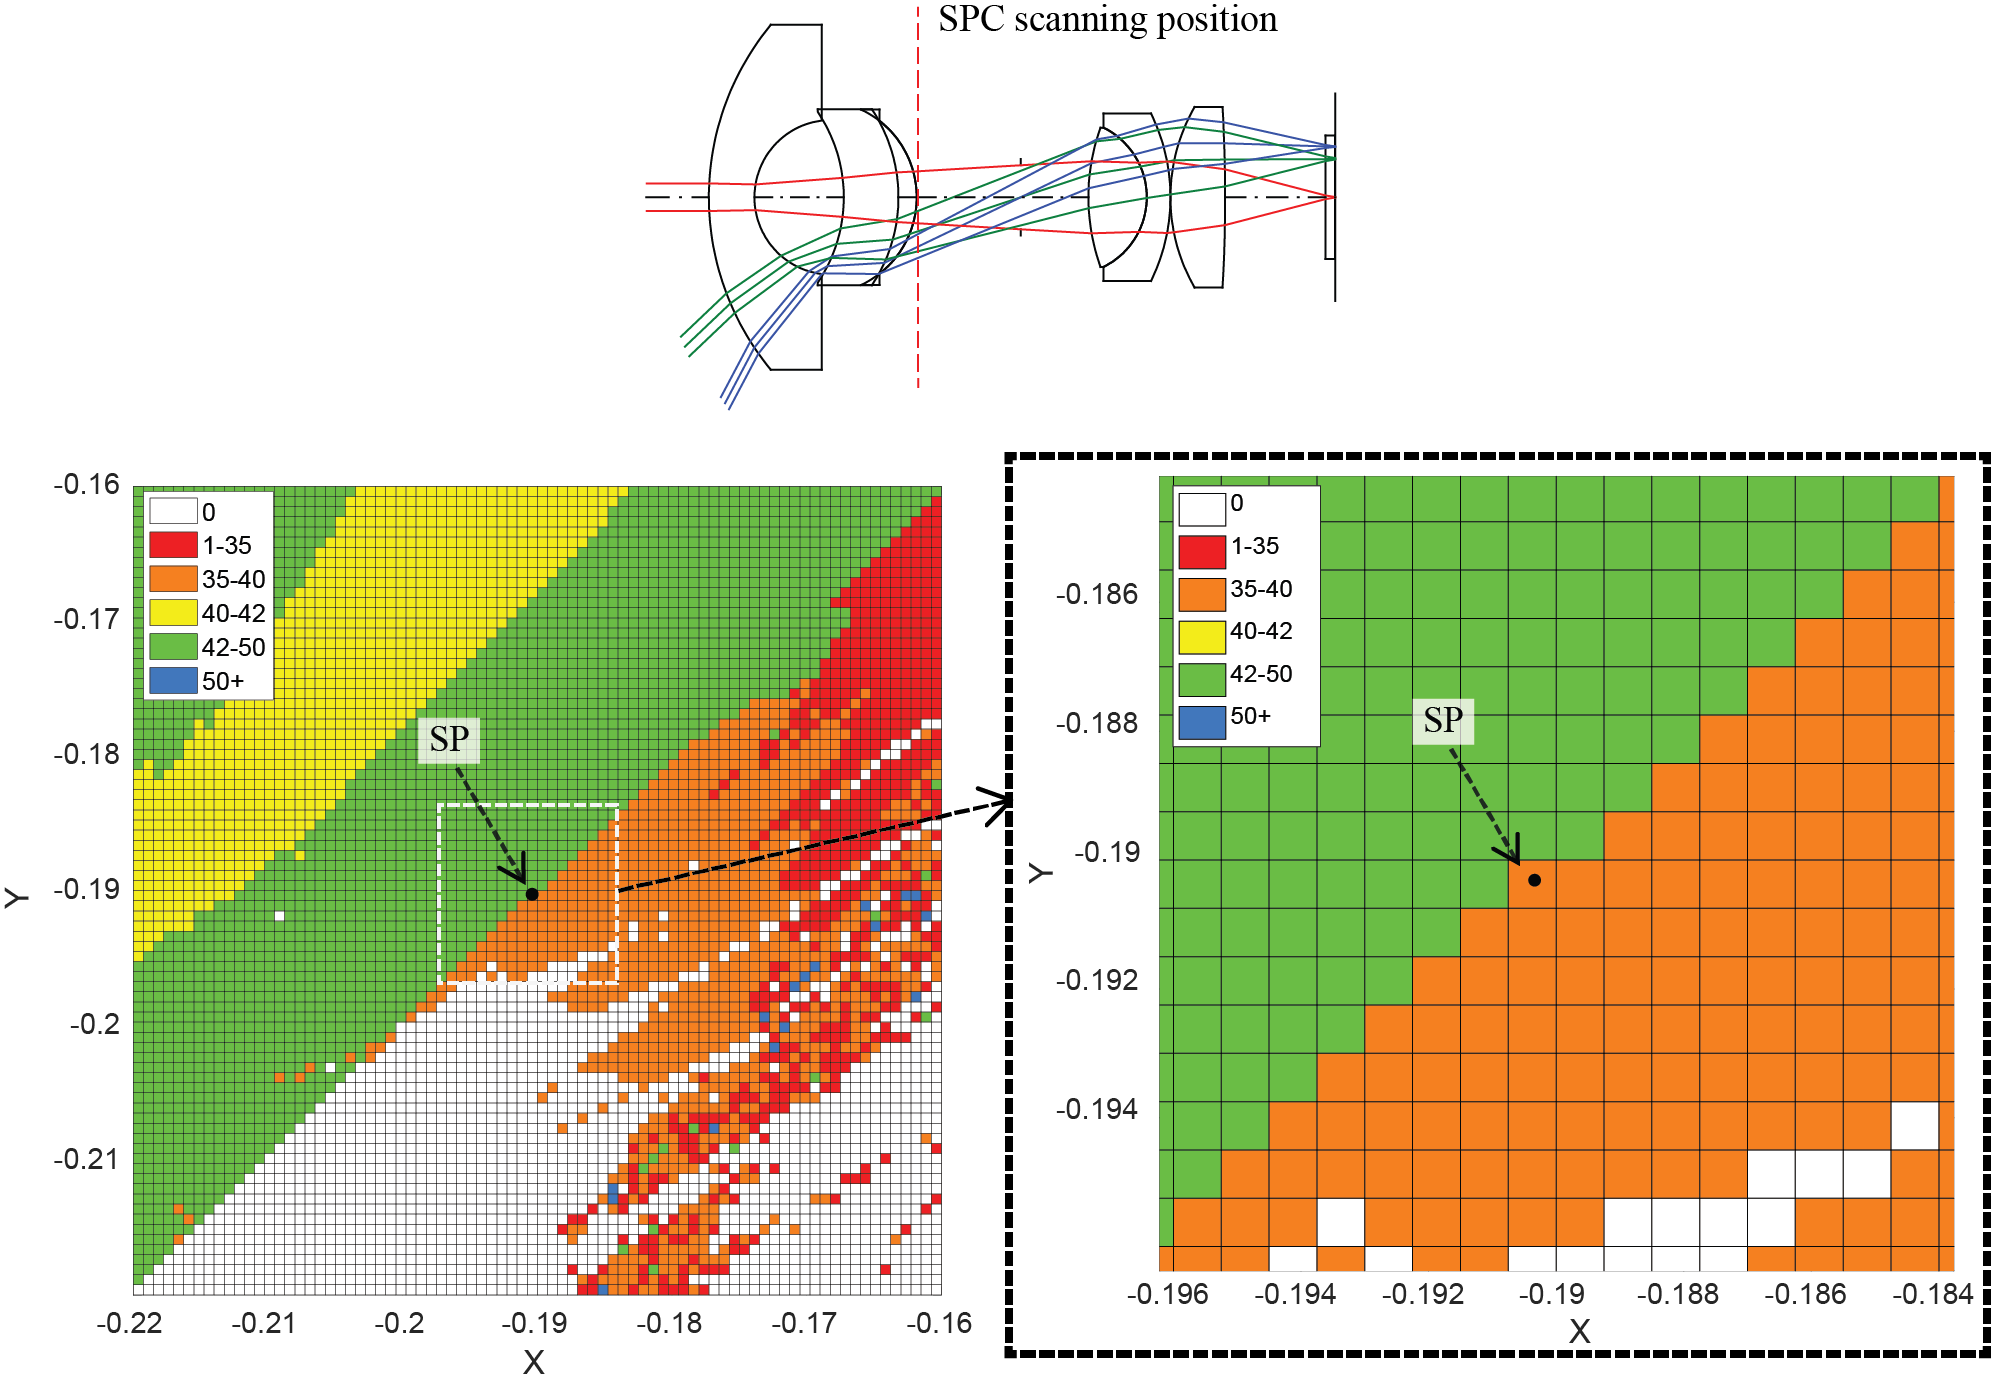
\includegraphics[width=0.8\textwidth]{chapter-4/figures/M3-S5_basins.png}
    \caption{Basins of attraction on the 2D plane defined by the inserted variables at a different scanning position compared to Figure \ref{fig:basins}. Along the scan line (diagonal line in the plot) around the saddle point, there are no starting points for which local optimization leads to minima other than the two next to the saddle point.}
    \label{fig:basins_WAL_M3_S5}
\end{figure}
\subsubsection{Discussion on Local Minima and the Thickness of the Inserted Element}
Until now, the mentioned minima are the minima with zero thickness for the inserted element. To obtain practical solutions, it is necessary to increase the thickness of the zero-thickness element to some nonzero values. In the example of this wide-angle lens, the thickness of the zero-thickness element in each local minimum is restored to the value of the original lens element before extraction. The number of the zero-thickness local minima and the number of local minima after increasing the thickness, are not the same. In Table \ref{table: scanline}, both the zero-thickness minima and the minima after increasing the thickness are listed. When the thickness is increased, T2-M1 merges with T2-M2, and so do T2-M3 and T2-M4. The final results become T2-MT1 and T2-MT2. T2-MT1 corresponds to M1 in Figure \ref{fig:WAL_network} with a merit function value of 4.20. T2-MT2 corresponds to M3 in Figure \ref{fig:WAL_network} with a merit function value of 8.58. 

Figure \ref{fig:thickness_increase} shows the change of merit function value when the thickness of the inserted element is increased in small steps (0.05 mm). In the left plot, the merit function value of T2-M3 changes drastically around thickness 2 mm. The system plots just before and after the peculiar value of  the thickness point are also illustrated in the same figure. Looking at the first lens element, it is seen that the system became very stressed (large curvature values) just before the thickness increased to 2 mm. Ray failure may occur when the thickness is further increased. In case of ray failure, CODE V adapted certain algorithms to modify the system in order to be able to trace the rays. In this example, the system T2-M3 merges with T2-M4 when the thickness is increased to more than 2 mm. On the right side of Figure \ref{fig:thickness_increase}, the merit function value of T2-M4 changes continuously with increasing thickness. The same phenomenon occurs with the other two systems: system T2-M2 merges with T2-M1 right after increasing the thickness. As previously illustrated in Figure \ref{fig:basins}, T2-M1 and T2-M4 correspond to the two expected local minima. It is worth mentioning that the two expected local minima are the two stable ones as shown in this example.

\subsubsection{Section Summary}
With a step by step analysis of applying SPC in this example, it is seen that, for some cases, choosing starting points on the SPC scan line may lead to unexpected local minima (zero-thickness). This may be caused by the specific landscape around the saddle point or numerical artefacts from the optimization algorithmn. Even though these problems do not always occur, examples suggest that a starting point should be chosen outside the scan line to prevent trapping in unwanted local minima. In the plotted basin of attraction, there are features that make the optimization around the saddle point unstable: optimization can reach to an unexpected local minimum or ray failure region. Therefore, choosing more than two starting points with proper distances to the saddle point is needed. In our experiment, we use four starting points: two are on the scan line and two are perpendicular to the scan line. The used distances to the saddle point curvatures are $2.5\%$ of the absolute value of the saddle point curvature (having a zero curvature is rarely the case in practice). In addition to the local optimization, experimental results also reveal that, in some cases, zero-thickness minima obtained in the intermediate steps of SPC are not stable and disappear after increasing the thickness of the inserted element. For the example given here, the final result (two finite-thickness minima) is less dependent on the precise choice of the starting points chosen after obtaining the saddle point.  

\begin{figure}[h!]
    \centering
    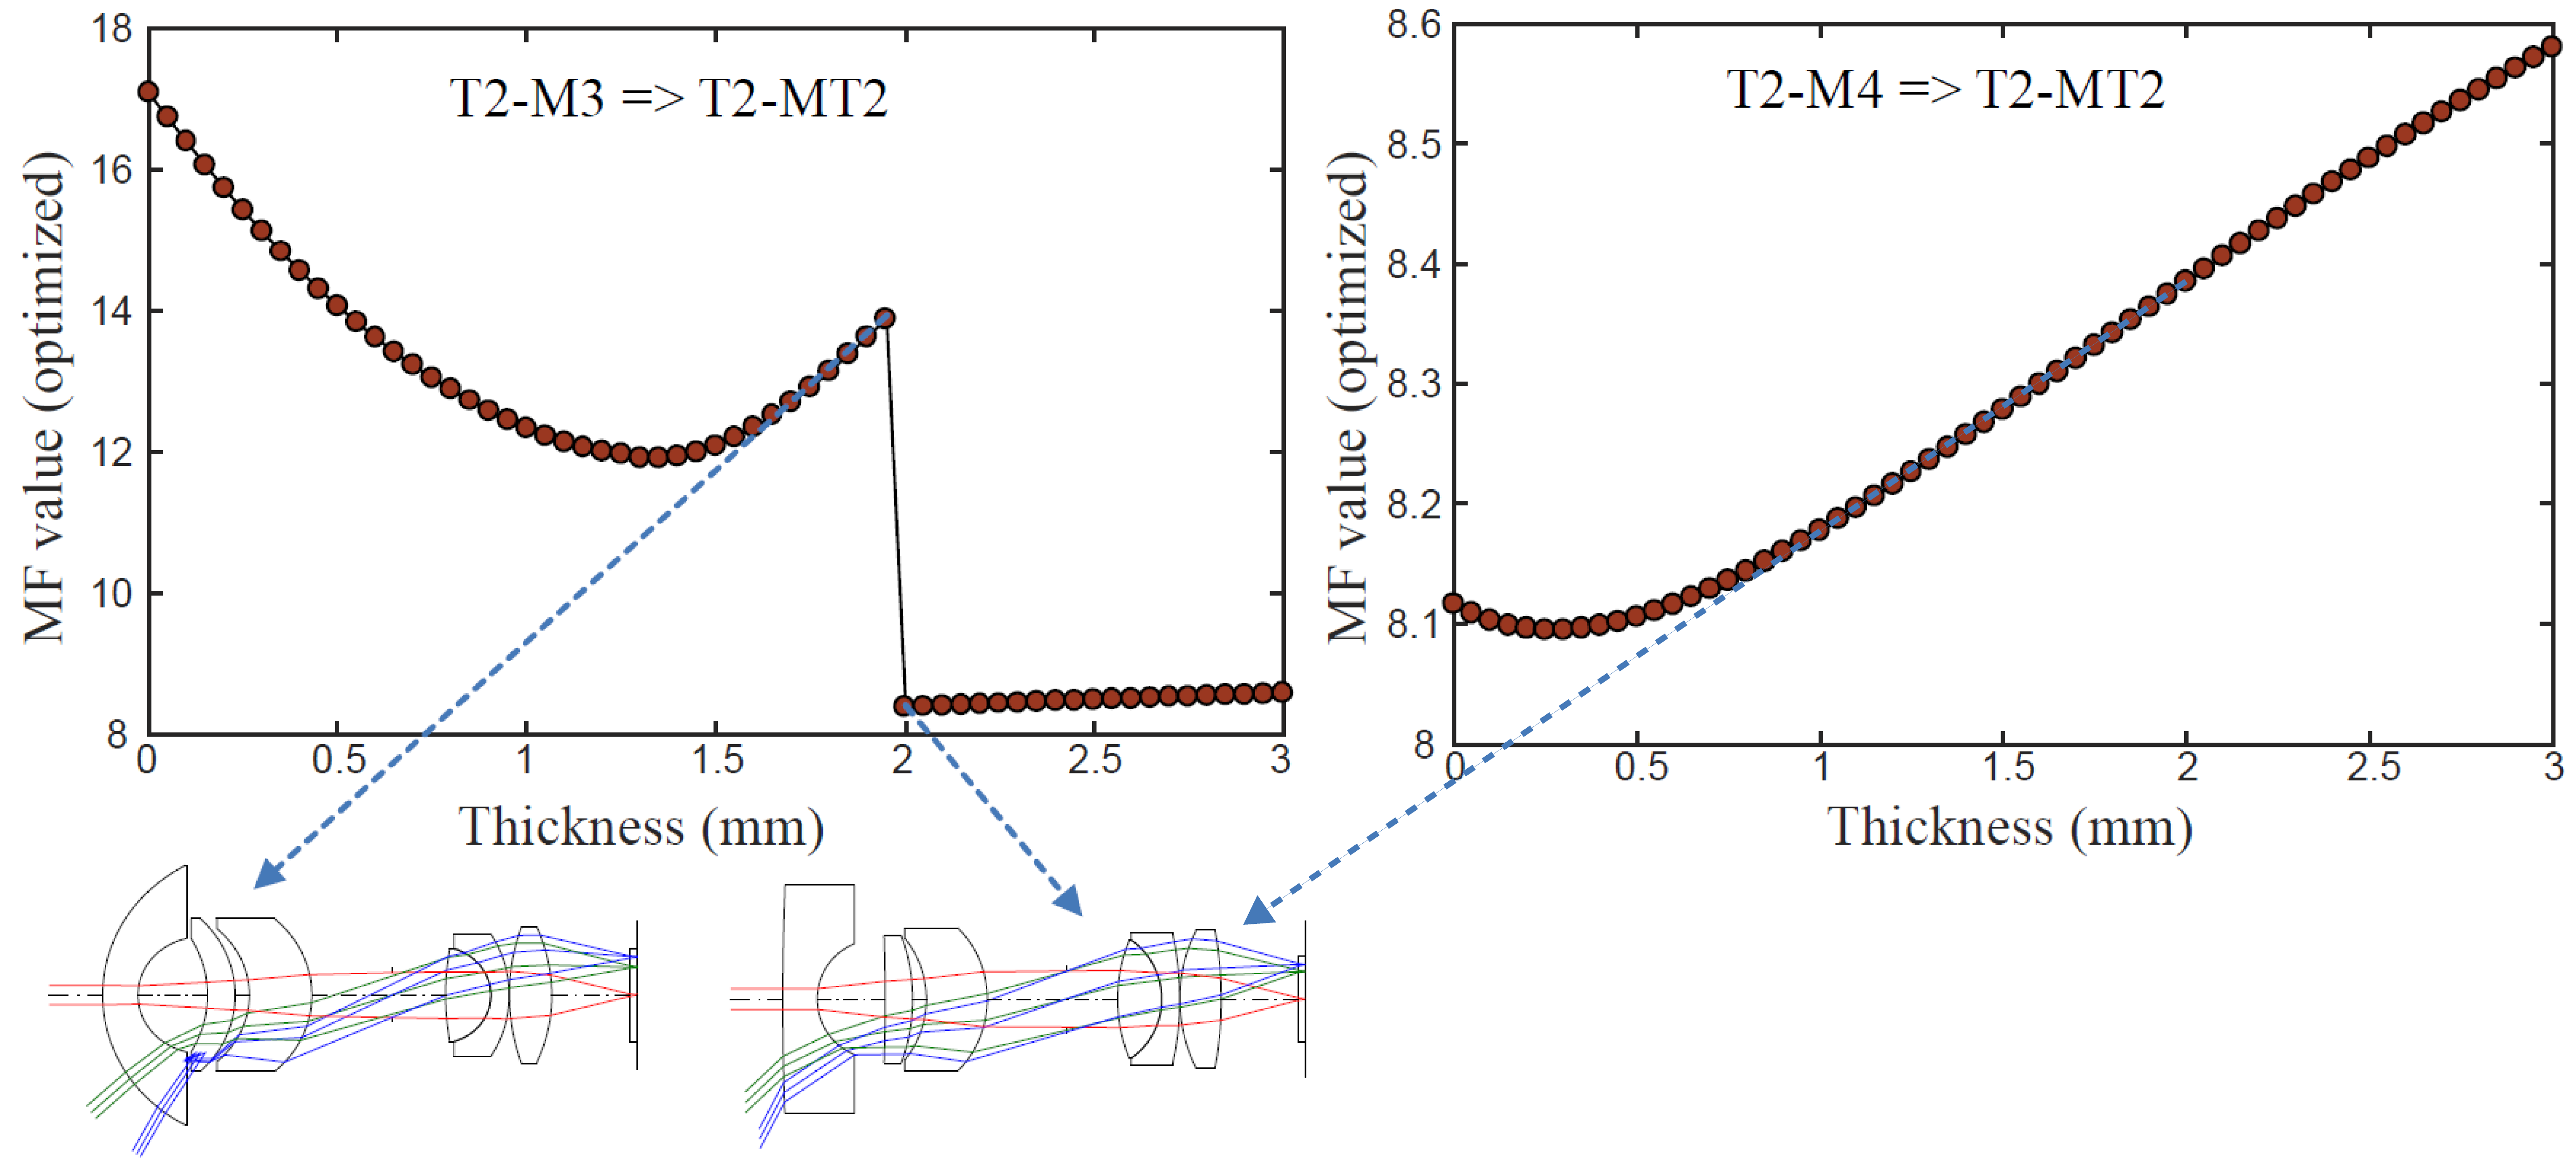
\includegraphics[width=0.8\textwidth]{chapter-4/figures/thickness_increase.png}
    \caption{Change of the optimized value of the merit function while increasing the thickness of the zero-thickness element. T2-M3 and T2-M4 correspond to systems when the thickness is zero. T2-MT2 corresponds to the system when the thickness equals 3 mm. The discontinuity of the left plot indicates the instability due to ray failure around a minimum in the design space. Systems like the left one are usually poor local minima.}
    \label{fig:thickness_increase}
\end{figure}

\section{Combining Designers' Knowledge and SPC to Improve Design Efficiency}
In lens design practice, it is common that multiple design techniques are applied to effectively obtain an optimal solution. The technique can be using a cemented doublet to reduce chromatic aberration, controlling the exit marginal ray angle to keep EFL constant, using a certain optimization method to find better local minima, etc. The SPC method provides a systematic approach to rapidly obtain local minima. However, it does not tell you where the SPC should be applied in an optical system. A straightforward way is to apply many SPCs in a system to generate all the possible local minima. However, this is not always preferred because at a certain phase of the design process, the designer does not really expect a drastic change of the system. In this section, we explore the option of combining designer knowledge and SPC. A UV dry microscope objective is used to show what can be achieved with this approach. 
%I have somehow an established system, where no big change is preferred to be made.  Only local/small adjustment is wanted in order to gain performance improvement. The "localness" depends on each design scenario. The knowledge of the designer is rather "converged" at that point, and deviation from the current system drastically would distract the designer from the current "flow" of thought. On the level of user experience, the global optimizer is not preferred at such a fine and delicate phase of the designing. It might be a good tool at the very beginning to provide ideas for the starting point of the whole design process. 
% In this sense, the SPC shows its advantage since it could help the designer at different stage of the design. It could be used as a tool to navigate a local region of the current design snapshot. The designer can keep her/his sense of control as well as getting acceptable deviations of the design. 

\subsection{Ultraviolet (UV) Microscope Dry Objective}
As a method to search for alternative solutions in lens design, SPC can be automated. In such a scenario, SPC could be used as a global search tool, where, after setting up all the specifications, the program would generate potential solutions for further selection. However, one of the challenges in using SPC, is to choose the proper position for inserting the null element. Conventional design approaches encounter a similar dilemma, namely: when a design process gets stagnated, how to modify the system (adding, extracting or changing) to improve the system? Optical designers usually use their unique insight and experience based on monitoring the aberration, ray properties etc. to make decisions on how to change the system. These approaches and methods used can be very different from person to person, therefore, setting up an algorithm to try out all promising looking options is difficult. If the optical system is relatively simple, it is possible to combine the SPC with approaches based on the designer's knowledge. To use SPC, the modification of the system should be adding or replacing lens elements in the existing system. In the following sections, we will provide two examples of how to combine SPC with conventional approaches. 

An ultra-violet (UV) microscope objective is chosen as a starting configuration. The microscope objective is taken from an existing patent\cite{patentvollrath} where its specification is reported. The variation designed for wavelength 325 nm is selected from the patent and reproduced in CODE V. The system consists of seven lens elements. The material used in CODE V is fused silica (LithosilQ from SCHOTT) with a refractive index of 1.4816 at 325 nm. The specification and performance of the system are listed in Table \ref{table: vollrathspec}. With a barrel lens having a focal length of 250 mm, the magnification of the composite microscope becomes 100. The seven lens elements of the system can be divided into three function groups according to a categorization method proposed by Zhang and Gross \cite{ZhangMicroscope2017}: the first lens on the left forms the rear group; the second and third lenses form the middle group, and the rest of the lens elements form the front group. The objective is shown in Figure \ref{fig: vollrathoriginal}. The front group is defined as the one facing to the object in the application, however, during the design it is convenient to work reversely, hence the front group is on the right side in Figure \ref{fig: vollrathoriginal}. According to the same author, existing microscopes can be categorized into three types depending on the functions performed by different groups of lenses. The distribution of the spherical aberration in different groups shown in Figure \ref{fig: vollrathoriginal} indicates that the middle and rear group compensate each other to correct the spherical aberration. This correction behaviour belongs to one of the types described in \cite{ZhangMicroscope2017}.

\setlength{\arrayrulewidth}{.5mm}
\setlength{\tabcolsep}{18pt}
\renewcommand{\arraystretch}{1.2}
\begin{table}[h!]
    \centering
    \captionsetup{justification=centering}
    \caption{System specification and performance of the microscope objective}
    \label{table: vollrathspec}
    \vspace{-1em}
    \begin{tabular}{ p{15em}  c }
    \hline 
    Effective Focal Length (mm) & 2.5\\ 
    Field (real image height, mm) & 0.1\\ 
    Numerical Aperture (NA) & 0.90\\ 
    Operating Wavelength (nm) & 325\\ 
    Working Distance (WD, mm) & 0.6\\ 
    Overall Length (mm) & 25\\
    \midrule
    RMS Wave Front Error (m\textlambda) & 49\\ 
    Strehl Ratio at 0 mm & 0.976\\ 
    Strehl Ratio at 0.1mm & 0.849\\
    \hline
    \end{tabular}
\end{table}

\begin{figure}[h!]
    \centering
    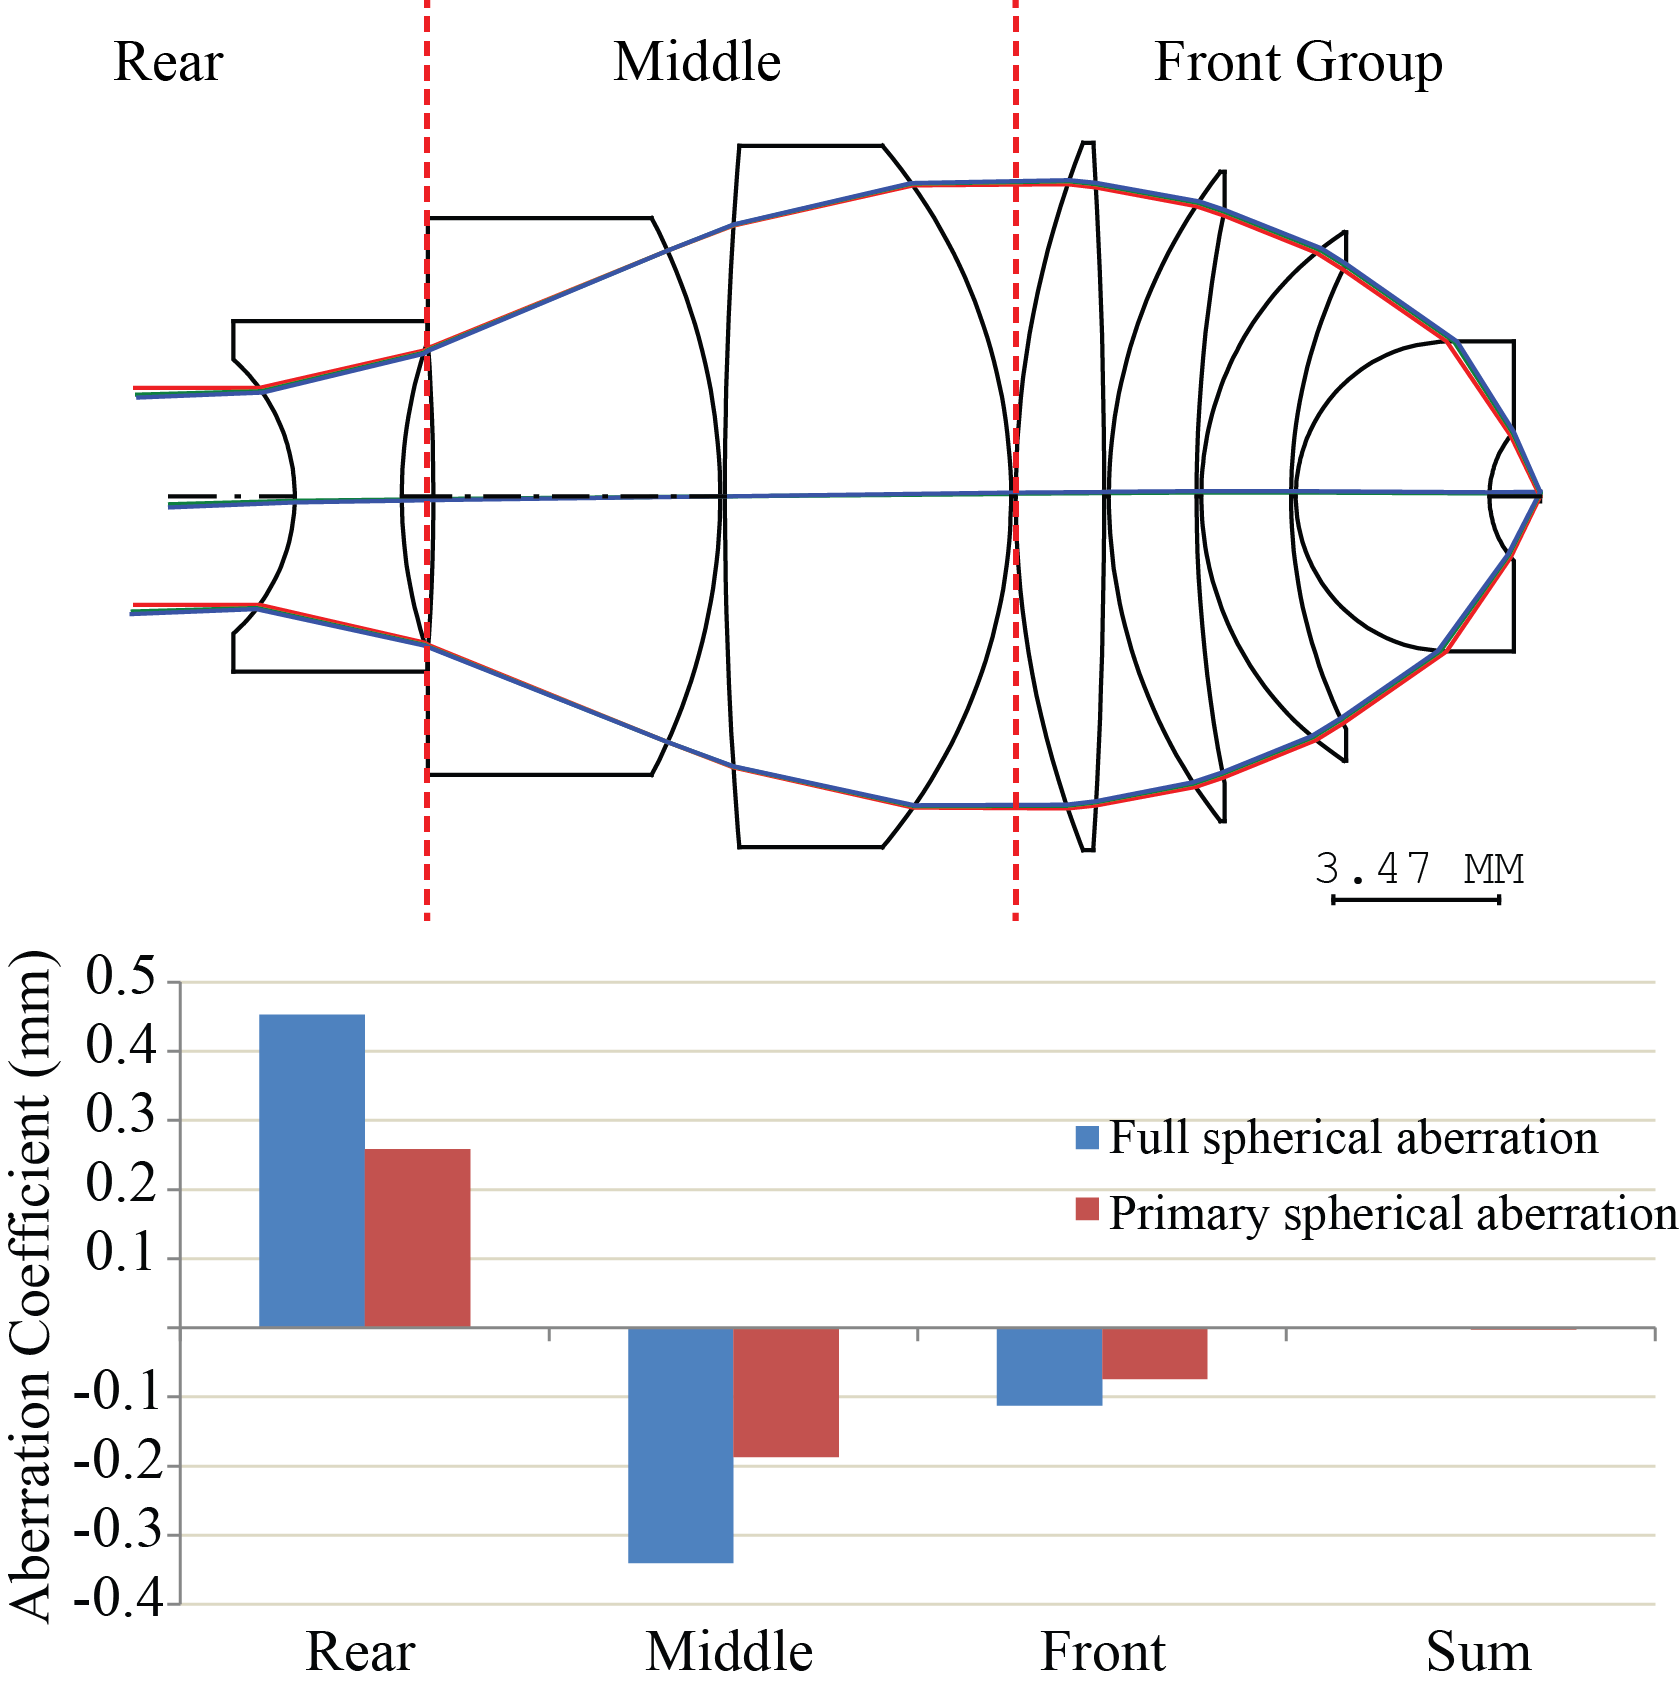
\includegraphics[width=0.55\textwidth]{chapter-4/figures/Vollrath_original.png}
    \caption{System plot of the UV microscope objective \cite{patentvollrath}. The objective can be divided into three groups of lenses. The rear group and middle group compensate each other to correct the spherical aberration \cite{ZhangMicroscope2017}.}
    \label{fig: vollrathoriginal}
\end{figure}

The current system already has a good performance and a compact size, its specifications are listed in Table \ref{table: vollrathspec}. However, if some of the specifications are made more demanding, a certain structural modification of the original system is necessary to keep a satisfactory performance. It is then interesting to investigate how SPC could help to find these modifications. The most simple case to investigate is to add an additional lens element. 

In contrast to a simple design problem, a complex system often needs several constraints to fulfill the design requirements. Before showing the design examples, the handling of constraints in SPC is first discussed in the following section.

\subsection{Constraints in Optical Design Software} \label{Constraints in optical design software}
The wide-angle lens shown in the previous section is a moderately complex system where SPC can be used in a limited number of positions. The system only has one requirement on the specifications that needs to be controlled, namely the EFL. It was controlled by setting the value of the exit angle $\alpha$  of the marginal ray on the last optical surface. Given the EPD and the EFL, the exit marginal ray angle $\alpha$ on the last optical surface can be set in CODE V as:
\setlength{\belowdisplayshortskip}{5pt}
\setlength{\abovedisplayshortskip}{5pt}
\begin{equation} \label{eq:EFLsolve}
\tan\alpha = \frac{EPD}{2\times EFL},
\end{equation}
\noindent Certain design requirements, such as EFL, can be used to force selected parameters to be dependent variables which are solved explicitly to keep the chosen requirements satisfied. In automatic design (optimization), this also makes it possible to reduce the number of independent variables, and thereby save computation effort.

However, in lens design practise, most of the design requirements cannot be explicitly controlled in the  aforementioned way. Constraint function such as equality constraint, inequality constraint, penalty function, etc. are then necessary to be implemented in order to fulfill the various requirements. In lens design software, there are usually different constraint functions for the user to choose so that it is possible to control the system design in different ways. In CODE V for example, there are four different types of constraint functions can be used as shown in Table \ref{table: codevconstraints}.

%table template
%\setlength{\arrayrulewidth}{.5mm}
%\setlength{\tabcolsep}{18pt}
%\renewcommand{\arraystretch}{1.2}
\begin{table}[h!]
    \centering
    \captionsetup{justification=centering}
    \caption{Different types of constraints in CODE V\cite{codevmanual}}
    \label{table: codevconstraints}
    \vspace{-1em}
    \begin{tabular}{ p{0.31\textwidth} | m{0.45\textwidth} }
    \hline 
    \textbf{Constraint Mode} & \textbf{Explanation}\\
    \hline
    Equality constraint (=) & Always active. Handled with Lagrangian Multiplier Method. Constrains exactly to target value of the constraint.  \\
    \hline
    Inequality constraint (>, <) & Only active when the optimization violates the targeted boundary. Handled with Lagrangian Multiplier Method.\\
    \hline
    Weighted function (WTC) & Only used for targeted constraint. Includes a weighted function in the merit function.\\
    \hline
    Penalty function (PTC) & Only used for targeted constraint. Includes a penalty function in the merit function. The penalty function is defined in CODE V with more tuning options than the weight function. It is essentially the same way of constraint implementation as the weight function.\\
    \hline
    \end{tabular}
\end{table}

As seen in Table \ref{table: codevconstraints}, both equality and inequality constraints are handled with the Lagrangian multiplier method. We will show in the following part that these two options treat the constraint by adding new variables to the optimization problem. To be compatible with the SPC scan requirement, one has to use the value of the Lagrange function instead of the original merit function. The penalty and weighted function methods treat the constraint by directly modifying the merit function. One can keep using the modified merit function for SPC scans. 

For SPC, before inserting the null element, it is necessary to optimize the current optical system to a local minimum with a given merit function. However, when the constraint is implemented using the Lagrange Multiplier method, it is necessary to use the Lagrange function (instead of the original merit function) to perform the SPC scan. We will explain the reasons for this in the following paragraphs. 

One of the advantages of using a Lagrange multiplier rule is that it treats  the constraint separately from the merit function, allowing the merit function to be based solely upon image quality-related criteria. For the case of an equality constraint, the optimization of the merit function can be written as follows:
\setlength{\belowdisplayshortskip}{5pt}
\setlength{\abovedisplayshortskip}{5pt}
\begin{equation} \label{eq: MFminCon}
\begin{split}
& \text{minimize}\;\; MF(\textbf{x}), \\
& \text{subject to}\;\; g(\textbf{x}) = 0,
\end{split}
\end{equation}
\noindent where $\textbf{x} = (x_1, x_2, ..., x_N)$ is a vector describing a point in the $N$-dimensional variable space. Equation $g(\textbf{x})=0$ is an equality constraint that the variables have to satisfy. Given that both $MF$ and $g$ have continuous first partial derivatives, a new variable $\lambda$ called a Lagrange multiplier is introduced, and the Lagrange function is defined by
\setlength{\belowdisplayshortskip}{5pt}
\setlength{\abovedisplayshortskip}{5pt}
\begin{equation} \label{eq: LagFun}
\mathcal{L}(\textbf{x},\lambda)=MF(\textbf{x})-\lambda\cdot g(\textbf{x}).
\end{equation}A critical point of Equation \ref{eq: LagFun} has zero gradient and satisfies the following equations
\setlength{\belowdisplayshortskip}{5pt}
\setlength{\abovedisplayshortskip}{5pt}
\begin{subequations} 
\begin{align}
& \nabla_\textbf{x}\mathcal{L}(\textbf{x},\lambda)=\nabla_\textbf{x}MF(\textbf{x})-\lambda\nabla_\textbf{x}g(\textbf{x})=0, \label{eq: LagCondition1} \\
& \nabla_\lambda\mathcal{L}(\textbf{x},\lambda)=g(\textbf{x})=0. \label{eq: LagCondition2}
\end{align}
\end{subequations}
From Equation \ref{eq: LagCondition2}, it is seen that once a critical point of $\mathcal{L}(\textbf{x},\lambda)$ is found, the equality constraint is automatically satisfied. Equation \ref{eq: LagCondition1} indicates that the gradient of the merit function can be expressed as a linear combination of the gradient of the constraints at the critical point. The Lagrange multiplier $\lambda$ acts as the coefficients. The Lagrange multiplier rule states that at the critical point, the value of the constrained merit function is either a maximum or minimum. 
%Note: It is equivalent to say that any direction perpendicular to the gradient of the constraint is perpendicular to the gradient of the merit function. 
In this way, the constrained optimization problem in Equation \ref{eq: MFminCon} is converted to an unconstrained optimization problem. The Lagrange Multiplier method converts the original $N$-dimensional problem into a $N+1$-dimensional problem by adding one more variable $\lambda$.  At the critical points of $\mathcal{L}(\textbf{x},\lambda)$, $\mathcal{L}(\textbf{x},\lambda)$ equals $MF(\textbf{x})$. Therefore, the smallest value of $\mathcal{L}(\textbf{x},\lambda)$ at the critical point gives the minimum of the constrained merit function. 

Before performing the SPC scan and adding the null element, the system needs to be firstly optimized to a local minimum. In CODE V, when equality or inequality constraints are applied, the Lagrange Multiplier method is used. The optimizer converges to a critical point satisfying Equations \ref{eq: LagCondition1} and \ref{eq: LagCondition2}. 

We would like now to investigate the possibility of $\nabla_\textbf{x}MF(\textbf{x}) = 0$ at a critical point of $\mathcal{L}(\textbf{x},\lambda)$. According to Equation \ref{eq: LagCondition1}, satisfying $\nabla_\textbf{x}MF(\textbf{x}) = 0$ requires either $\lambda =0 \;\; \text{or} \;\; \nabla_\textbf{x}g(\textbf{x})=0$. Given Equation \ref{eq: LagCondition2} is valid, either condition $\lambda = 0$ or $\;\; \nabla_\textbf{x}g(\textbf{x})=0$ indicates that the local minimum of the original unconstrained merit function ($MF$) coincides with the local minimum of the Lagrange function. Therefore, the constraint is already fulfilled at the local minimum of the original merit function. It indicates Lagrange function is in practice not needed for this situation and this situation is not in general valid when Lagrange function is applied. As a results, $\nabla_\textbf{x}MF(\textbf{x}) \ne 0$ is the typical situation for a critical point of $\mathcal{L}(\textbf{x},\lambda)$. It indicates that the unconstrained merit function is not at its local minimum.  

When performing the SPC scan, two additional variables ($c_1$ and $c_2$, curvatures of the null element) are added to the existing system. In ray tracing software like CODE V, the user usually only sees the value of the merit function. In a case that Lagrange Multiplier method is used, if the SPC scan of the saddle point uses the unconstrained merit function, the construction of the saddle point will not start from a local minimum. The precondition for performing the SPC is thus not satisfied and saddle points will not be obtained. As a recommendation, when Lagrange Multiplier method is used, the SPC scan should be performed using the Lagrange function.  
% the only fundamental issue would be that if the g(x) conflicts with the null-element condition. At the null-element, the g(x) should still be valid. Practically, I don't see how it will happen. 

The inequality constraint mentioned in Table \ref{table: codevconstraints} should take the same situation into consideration: The constraint becomes active when the optimization violates the boundary, and the computation for SPC scan should use the Lagrange function; The constraint remains inactive if the optimization is operated within the defined boundary, and the original merit function is used for SPC scan. 

When constraints are implemented using a penalty function or a weighted function method, the preconditions for performing SPC are satisfied. Both approaches add new terms to the merit function with explicit expressions. The altered merit function is used to optimize the system to a local minimum and the same function is used to perform SPC. 

The modified merit function with a weight function term can be written as the following 
\setlength{\belowdisplayshortskip}{5pt}
\setlength{\abovedisplayshortskip}{5pt}
\begin{subequations} 
\begin{align}
& MF_{W}(\textbf{x})=MF(\textbf{x})+\sum_{i=1}^{m}W_i(\textbf{x}), \label{eq: MFWeight} \\
& W(\textbf{x})=(wt\cdot \Delta C)^2. \label{eq: WTC}
\end{align}
\end{subequations}
where the summation indicates that multiple weight functions can be added, $wt$ is the weighting factor set in CODE V, and $\Delta C$ is the departure of the constraints from its target. Using the penalty function replaces the weight function term in Equation \ref{eq: MFWeight} with a penalty function described as the following in CODE V
\setlength{\belowdisplayshortskip}{5pt}
\setlength{\abovedisplayshortskip}{5pt}
\begin{equation} \label{eq: PTC}
P = wt*(\frac{\Delta C}{half \, width})^{\frac{exponent}{2}},
\end{equation}where ${half \, width}$ and $exponent$ are two additional variables for tuning the penalty function. If the ${half \, width}$ is set to $1$ and the $exponent$ is set to $4$, the penalty function in Equation \ref{eq: PTC} is the same as the weight function in Equation \ref{eq: WTC}. The two approaches for implementing the constraints are essentially identical. They both provide a less rigid control compared to the Lagrange Multiplier method. The penalty function mode is ideal for the "soft constraints", which are constraints that have an acceptable range of values \cite{codevmanual}. 

As described in this section, applying constraints using Lagrange Multiplier method needs additional engineering treatment to be compatible with SPC scans. We prefer to use weighted or penalty function for its simplicity of keeping track of the same merit function. In the rest of this chapter, where different constrained systems are investigated, the constraints are implemented with the weighted function.

\subsection{Applying SPC to Induce Structural Changes in Lens}
%add some text to elaborate the title
When trapped in a local minimum, it is useful to introduce structural change in order to obtain different local minima with significant changes in the values of the merit function. The structural change refers to changes such as using a lens with a positive power instead of a negative one, adding a new element into the system, etc. In this section, we focus on two cases where structural changes are needed for the systems to meet a higher requirement. In the first case, the NA of the system is further increased from 0.90 to 0.95. In the second case, the working distance of the system is increased from 0.6 mm to 2.5 mm. We show how SPC can be effectively applied to obtain new local minima. 
%We demonstrate that SPC

\subsubsection{Increasing NA of the Objective}
For a high-resolution microscope objective, high NA is always required. The first example is to increase the NA of the microscope objective from 0.90 to 0.95. The rays can still be traced after the modification, i.e. in the case considered no ray failure occurs after the increase of the NA. The system is then optimized with a wavefront error function. An EFL constraint and a working distance constraint are applied with the equality constraint mode. Figure \ref{fig: vollrathNA90295} shows that the change of the system shape \footnote{A system shape is determined by the bending of each lens element, the thicknesses of the lens elements and  the distance between them.} is mainly in the thickness of the elements. The bending \footnote{The definition of the bending factor is given in Equation \ref{eqn: bending factor}.} of each element remains almost unchanged. From Table \ref{table: NAchange}, it is seen that the performance of the system deteriorates after increasing the NA. A major cause is that the spherical aberration (especially the high-order spherical aberration) increases with increasing NA. In traditional approaches, structural changes to the system would be made by which the number of degrees of freedom increases to be able to reduce the aberration. These kinds of structural change could, for example, be replacing a spherical surface by an asphere, adding extra lens elements, or splitting existing lens elements. In the following examples, the introduced changes are adding or splitting lens elements.

\begin{figure}[h!]
    \centering
    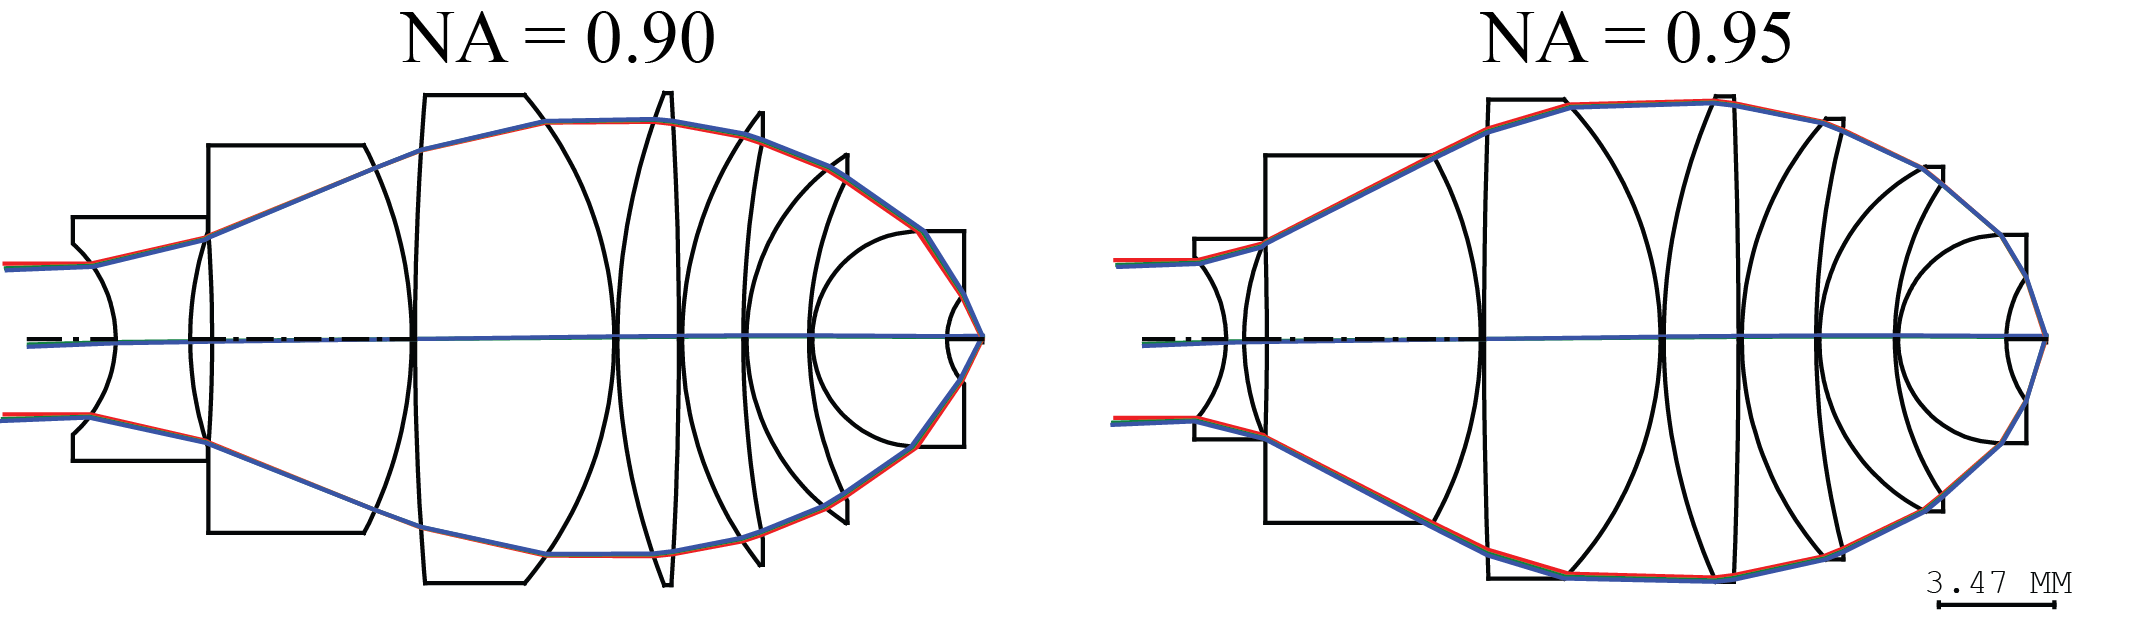
\includegraphics[width=0.6\textwidth]{chapter-4/figures/Vollrath_NA90295.png}
    \caption{Change of the system shape after increasing the NA from 0.90 to 0.95.}
    \label{fig: vollrathNA90295}
\end{figure}

%table template
\setlength{\arrayrulewidth}{.5mm}
\setlength{\tabcolsep}{18pt}
\renewcommand{\arraystretch}{1.2}
\begin{table}[h!]
    \centering
    \captionsetup{justification=centering}
    \caption{Change of the system performance with increasing NA}
    \label{table: NAchange}
    \vspace{-1em}
    \begin{tabular}{ c c c }
    \hline 
     Numerical Aperture & 0.90 & 0.95\\ 
     \cmidrule{2-3}
    RMS Wavefront Error (m\textlambda) & 49 & 111  \\ 
    Strehl Ratio at 0 mm & 0.976 & 0.833\\
    Strehl Ratio at 0.1 mm & 0.849 & 0.386\\
    \hline
    \end{tabular}
\end{table}

With the separation of the system into different function groups, it is possible to understand the function of different parts of the system which provides insight when structural change is needed. It follows from Figure \ref{fig: vollrathoriginal} that the rear and middle group compensate each other to correct the spherical aberration. A reasonable strategy is then to introduce structural changes in these two groups, namely by adding or splitting elements in the rear and the middle group of the system. Based on this insight, four different positions are chosen in the rear and the middle group to add or split elements in the usual way. The resulted system shapes are shown in Figure \ref{fig: vollrathNAtrad}. It is worth pointing out that with the traditional approach of adding or splitting lens, each operation only yields one solution. The performance of the resulting systems are listed in Table \ref{table: vollrathNAtrad}. The data from the table reveal that out of four, one (the number 4 system) has satisfactory performance. For a satisfactory performance, the criteria used here are that the Strehl ratio is above 0.8 for all fields and the wavefront RMS is below $\lambda/14$ \cite{patentvollrath}, for which value the system is considered to be diffraction-limited. In Figure \ref{fig: vollrathNAtrad}, the inserted or split element is highlighted by shading. For operation \circled{1}, the insertion of the lens results in an additional shell lens in the front group. It gives four new degrees of freedoms (two curvatures, one lens thickness, and an air space thickness) for optimization. However, the performance of the optimized system is not satisfactory. Operation \circled{2} splits one of the lens elements in the middle group and thereby distributing its original power to two lens elements. The same happens in the case of operation \circled{3}. Both operations \circled{2} and \circled{3} produce only slightly better results than operation \circled{1}, however, neither of them is good enough. Splitting the lens element in the rear group in operation \circled{4} produces a different system shape compared to the other three and the original system. A reverse-bended element is created (second element from the left), which forms a narrow air gap with the element to the right of it. This kind of air gap is effective for introducing high-order spherical aberrations, which balances the high-order spherical aberrations introduced by other parts of the system \cite{ZhangGross+2019+349+384}. 

\begin{figure}[h!]
    \centering
    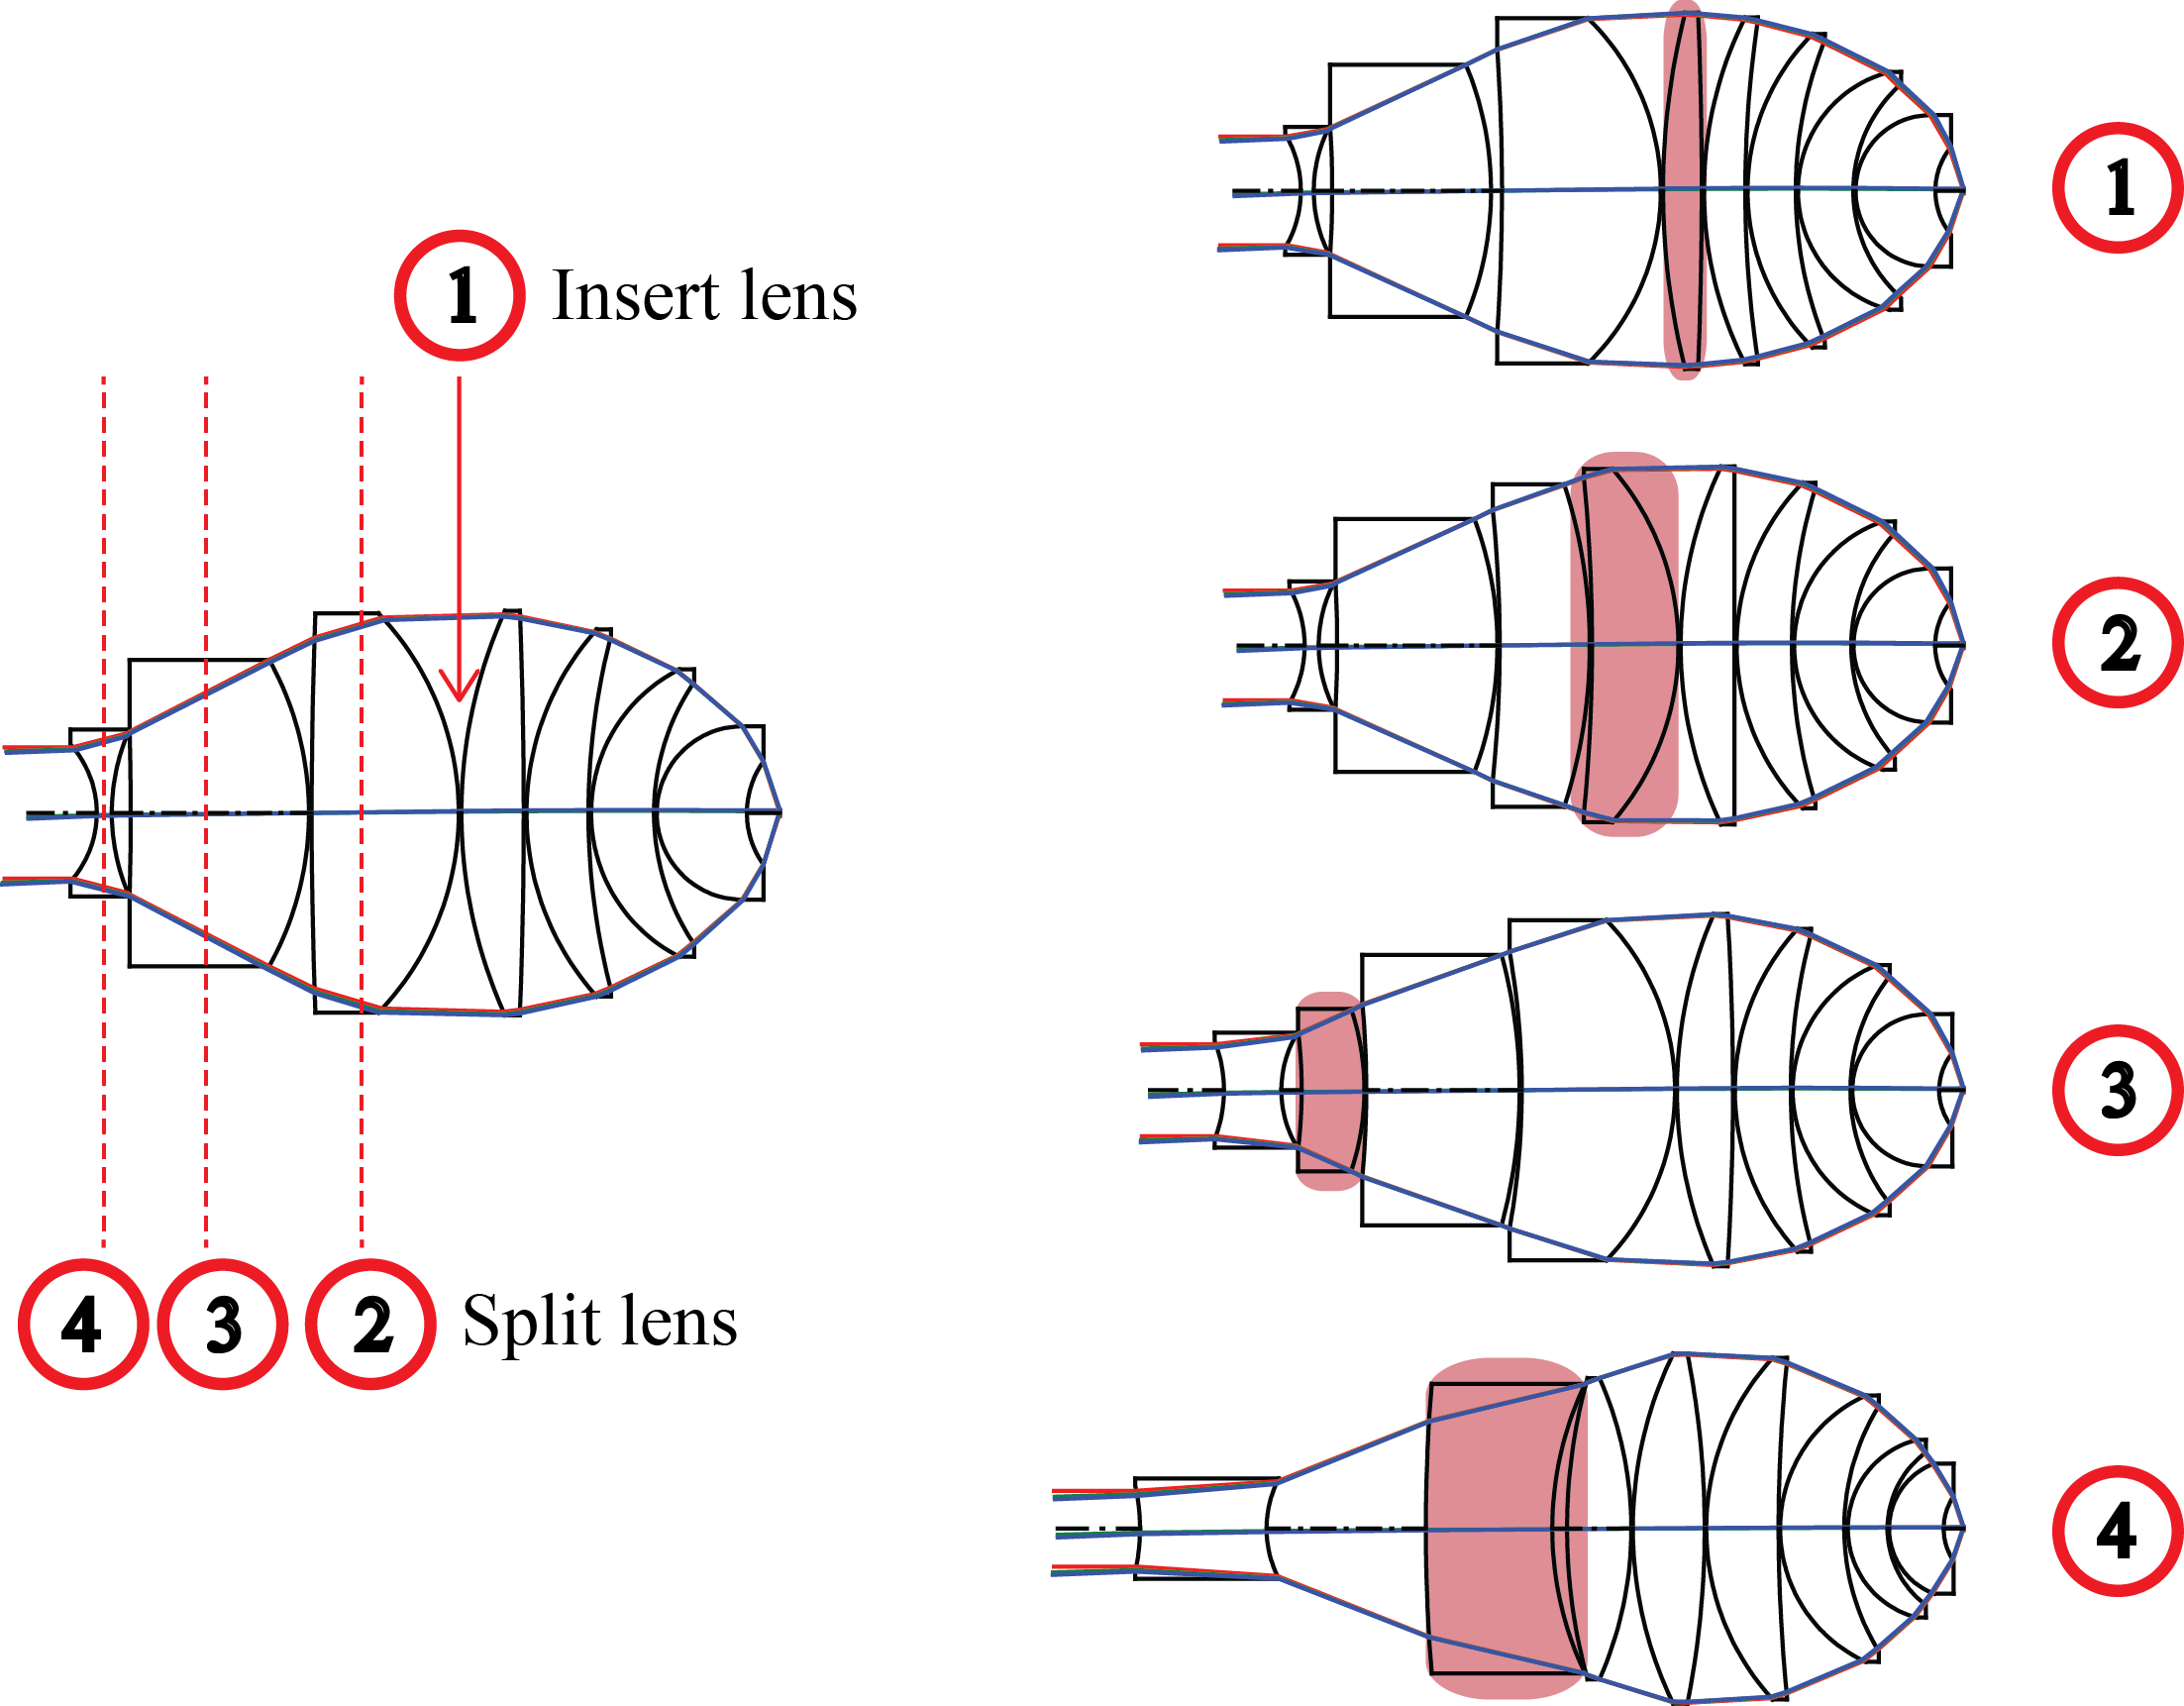
\includegraphics[width=0.7\textwidth]{chapter-4/figures/Vollrath_NATradition.png}
    \caption{Introducing structural change in the traditional way for system performance improvement. Four operations have been executed on the NA 0.95 system resulting in four different results. The inserted or split element is highlighted by shading.}
    \label{fig: vollrathNAtrad}
\end{figure}

\setlength{\arrayrulewidth}{.5mm}
\setlength{\tabcolsep}{18pt}
\renewcommand{\arraystretch}{1.2}
\begin{table}[h!]
    \centering
    \captionsetup{justification=centering}
    \caption{System performance for the systems shown in Figure \ref{fig: vollrathNAtrad}}
    \label{table: vollrathNAtrad}
    \vspace{-1em}
    % \hspace*{-10pt} %adjusting the position of the plot(table) !!!!
    \begin{adjustbox}{max width=\textwidth, center}
    \begin{tabular}{c c c c c}
    \hline 
     No. & \textbf{1} & \textbf{2} & \textbf{3} & \textbf{4}\\ 
     \midrule
    RMS Wavefront Error (m\textlambda) & 119 & 117 & 99 & 41 \\ 
    Strehl Ratio at 0 mm & 0.736 & 0.769 & 0.832 & 0.985\\
    Strehl Ratio at 0.1 mm & 0.428 & 0.453 & 0.548 & 0.882\\
    \hline
    \end{tabular}
    \end{adjustbox}
\end{table}

Based on the insight on where the change should be introduced in the system, SPC scans were performed at four positions in the system. Figure \ref{fig: VollrathSPCcaseNA} presents the results from SPC scans. From four scans, a total number of eighteen solutions were obtained. Besides four solutions which are identical to the ones obtained with the traditional method, fourteen extra solutions were obtained. Their performance is listed in Table \ref{table: vollratSPCcaseNA}. Out of the eighteen solutions, nine reach satisfactory results. Solution \circle{4}A and \circle{4}D even show better performance than the best one obtained by the traditional method (No.4 in Table \ref{table: vollrathNAtrad}). Among all the solutions, \circled{1}A and \circled{2}B have very close system shapes. One is the result from the left bending of the glass lens, and the other is the result of the right bending of the air lens. As explained in Chapter \ref{chapter_SPC_method_reccomendation}, there are two different ways to apply SPC, which lead to the same solution in this case.

\begin{figure}
  \begin{adjustbox}{addcode={
    \begin{minipage}{\width}}{
    \captionsetup{margin=0em}
    \caption{Eighteen solutions from four SPC scans. The dashed line indicates constructing an air lens inside a lens element (equivalent to splitting lens). The solid line indicates constructing a glass element in the air space (equivalent to add lens). In comparison with Figure \ref{fig: vollrathNAtrad}, solution \textcircled{\scriptsize{1}}C, \textcircled{\scriptsize{2}}D, \textcircled{\scriptsize{3}}C, and \textcircled{\scriptsize{4}}D are the ones obtained with conventional approach.}\label{fig: VollrathSPCcaseNA}
    \end{minipage}},rotate=90,center}
    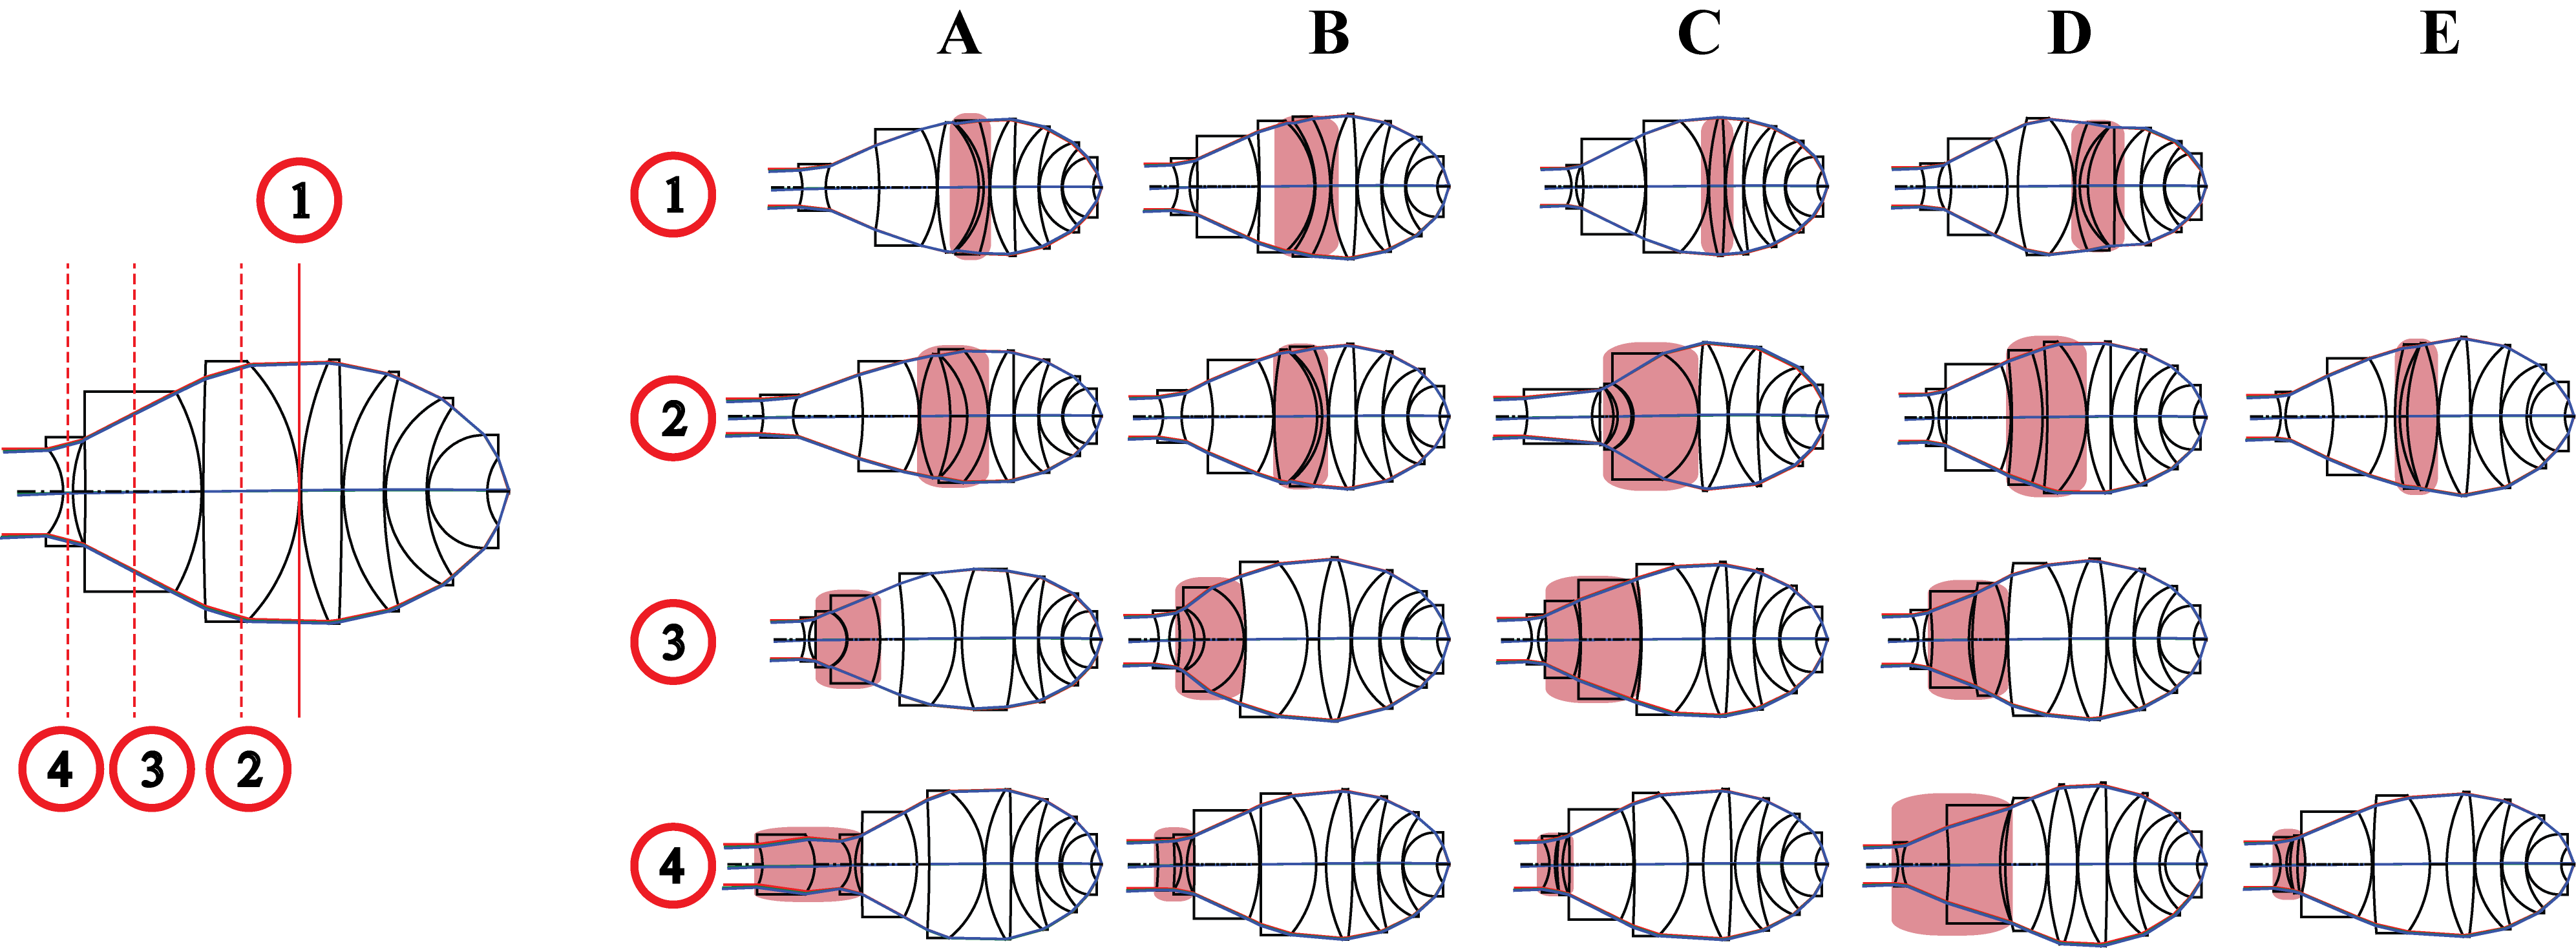
\includegraphics[width=0.96\textheight]{chapter-4/figures/vollrathSPCcaseNA.png}
  \end{adjustbox}
\end{figure}

\setlength{\arrayrulewidth}{.5mm}
\setlength{\tabcolsep}{18pt}
\renewcommand{\arraystretch}{1.2}
\begin{table}[h!]
    \centering
    \captionsetup{justification=centering}
    \caption{System performance for the systems shown in Figure \ref{fig: VollrathSPCcaseNA}}
    \label{table: vollratSPCcaseNA}
    \vspace{-1em}
    % \hspace*{-10pt} %adjusting the position of the plot(table) !!!!
    \begin{adjustbox}{max width=\textwidth, center}
    \begin{tabular}{c c c c c c}
    \hline 
       & \textbf{1} & \textbf{2} & \textbf{3} & \textbf{4} & \\ 
     \midrule
    RMS WFR & 65 & 59 & 60 & 26 & \multirow{3}{*}{\textbf{A}} \\ 
    SR(0) & 0.862 & 0.942 & 0.958 & 0.998\\
    SR(0.1) & 0.829 & 0.807 & 0.808 & 0.945\\
    \midrule
    RMS WFR& 109 & 67 & 52 & 135 & \multirow{3}{*}{\textbf{B}} \\ 
    SR(0) & 0.876 & 0.941 & 0.960 & 0.604\\
    SR(0.1) & 0.378 & 0.756 & 0.847 & 0.319\\
    \midrule
    RMS WFR & 98 & 45 & 104 & 124 & \multirow{3}{*}{\textbf{C}} \\ 
    SR(0) & 0.826 & 0.989 & 0.779 & 0.661\\
    SR(0.1) & 0.505 & 0.874 & 0.540 & 0.371\\
    \midrule
    RMS WFR & 48 & 102 & 89 & 35 & \multirow{3}{*}{\textbf{D}} \\ 
    SR(0) & 0.950 & 0.828 & 0.820 & 0.993\\
    SR(0.1) & 0.859 & 0.444 & 0.625 & 0.894\\
    \midrule
    RMS WFR &  & 43 &  & 135 & \multirow{3}{*}{\textbf{E}} \\ 
    SR(0) &  & 0.982 &  & 0.789\\
    SR(0.1) &  & 0.853 &  & 0.251\\
    \hline
    \multicolumn{6}{c}{\textit{\footnotesize{RMS WFR = RMS Wavefront Error (m\textlambda); SR(0) = Strehl Ratio at 0 mm; SR(0.1) = Strehl Ratio at 0.1 mm.}}}\\
    % \vspace{-1em}
    % \multicolumn{6}{c}{\textit{\footnotesize{SR(0) = Strehl ratio at 0 mm; SR(0.1) = Strehl ratio at 0.1 mm.}}}
    \end{tabular}
    \end{adjustbox}
\end{table}

Compared to the traditional method, more than 4 times as many systems are obtained for a comparable amount of computational load with SPC than with the traditional method. Besides the good solutions which are similar to the ones obtained with the traditional method, SPC also found eight additional solution with satisfactory performance. 

\newpage
\subsubsection{Increasing the Working Distance of the Objective}
A second structural change is introduced in the case of an increase of the working distance of the original system ( the system on the left in Figure \ref{fig: vollrathNA90295}), from 0.6 mm to 2.5 mm. This requires that the first lens element on the right is aplanatic-concentric instead of plano-concentric, causing a necessary decrease of power of the first element. In order to maintain the performance, this decrease of optical power need to be compensated. This is done by increasing the optical power of the lens element after the first one and those in the middle group. With the limited number of degrees of freedom, the performance of the system strongly deteriorates. Figure \ref{fig: vollrathWD06to25} shows how the system changed after increasing the working distance from 0.6 mm to 2.5 mm. The OverAll Length (OAL) of the system increases from 25 mm to 76 mm. The diameter of the maximum element increases from 6.6 mm to 17 mm. A longer air gap emerges after the first element on the left caused by the increase of the size (diameter) of the lens elements. The third lens element from the left is compressed into a thinner element. The bending of each element still remains close to that of the original system. Table \ref{table: vollrathWDchange} gives the change of the performance with the increase of the working distance. 

\begin{figure}[h!]
    \centering
    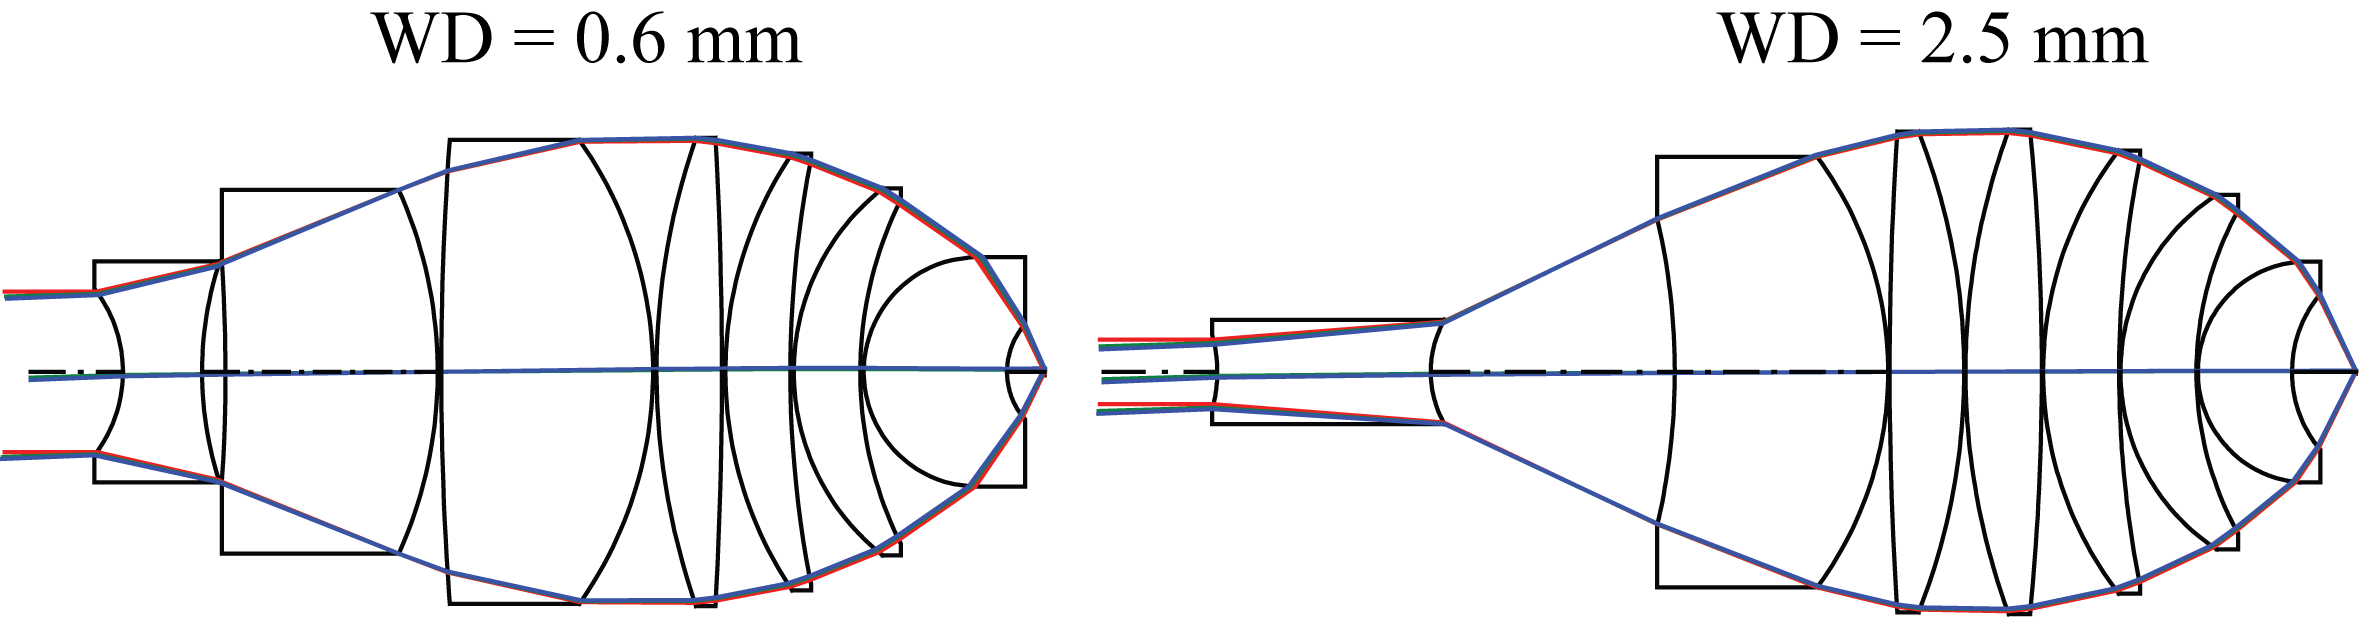
\includegraphics[width=0.75\textwidth]{chapter-4/figures/Vollrath_WD06TO25.png}
    \caption{Change of the system shape after the increasing of the working distance from 0.6 mm to 2.5 mm.}
    \label{fig: vollrathWD06to25}
\end{figure}

%table template
\setlength{\arrayrulewidth}{.5mm}
\setlength{\tabcolsep}{18pt}
\renewcommand{\arraystretch}{1.2}
\begin{table}[h!]
    \centering
    \captionsetup{justification=centering}
    \caption{Change of the system performance with increasing working distance}
    \label{table: vollrathWDchange}
    \vspace{-1em}
    \begin{tabular}{ c c c }
    \hline 
     Working distance (WD, mm) & 0.6 & 2.5\\ 
     \cmidrule{2-3}
    RMS wavefront error (m\textlambda) & 49 & 135  \\ 
    Strehl ratio at 0 mm & 0.976 & 0.254\\
    Strehl ratio at 0.1 mm & 0.849 & 0.019\\
    \hline
    \end{tabular}
\end{table}

To compensate for the decreased optical power of the first element, a common practice to introduce changes to the system for system improvement is to introduce a structural change in the middle or front group. By splitting or adding lens elements, newly added degrees of freedom will help to correct the aberrations. Two insertion positions and one splitting position were chosen for adding new degrees of freedom to the system. Figure \ref{fig: vollrathWDTrad} presents the results of the three operations: two insertions led to the same solution; the splitting shows a different system with good performance. The data of the system are listed in Table \ref{table: vollrathWDTrad}.

\setlength{\arrayrulewidth}{.5mm}
\setlength{\tabcolsep}{18pt}
\renewcommand{\arraystretch}{1.2}
\begin{table}[h!]
    \centering
    \captionsetup{justification=centering}
    \caption{System performance for the systems shown in Figure \ref{fig: vollrathWDTrad}}
    \label{table: vollrathWDTrad}
    \vspace{-1em}
    % \hspace*{-10pt} %adjusting the position of the plot(table) !!!!
    \begin{adjustbox}{max width=\textwidth, center}
    \begin{tabular}{c c c}
    \hline 
     No. & \textbf{1 \& 2} & \textbf{3}  \\ 
     \midrule
    RMS Wavefront Error (m\textlambda) & 100 & 41 \\ 
    Strehl Ratio at 0 mm & 0.833 & 0.975 \\
    Strehl Ratio at 0.1 mm & 0.507 & 0.902 \\
    \hline
    \end{tabular}
    \end{adjustbox}
\end{table}

\newpage % adjust page arrangement

\begin{figure}[h!]
    \centering
    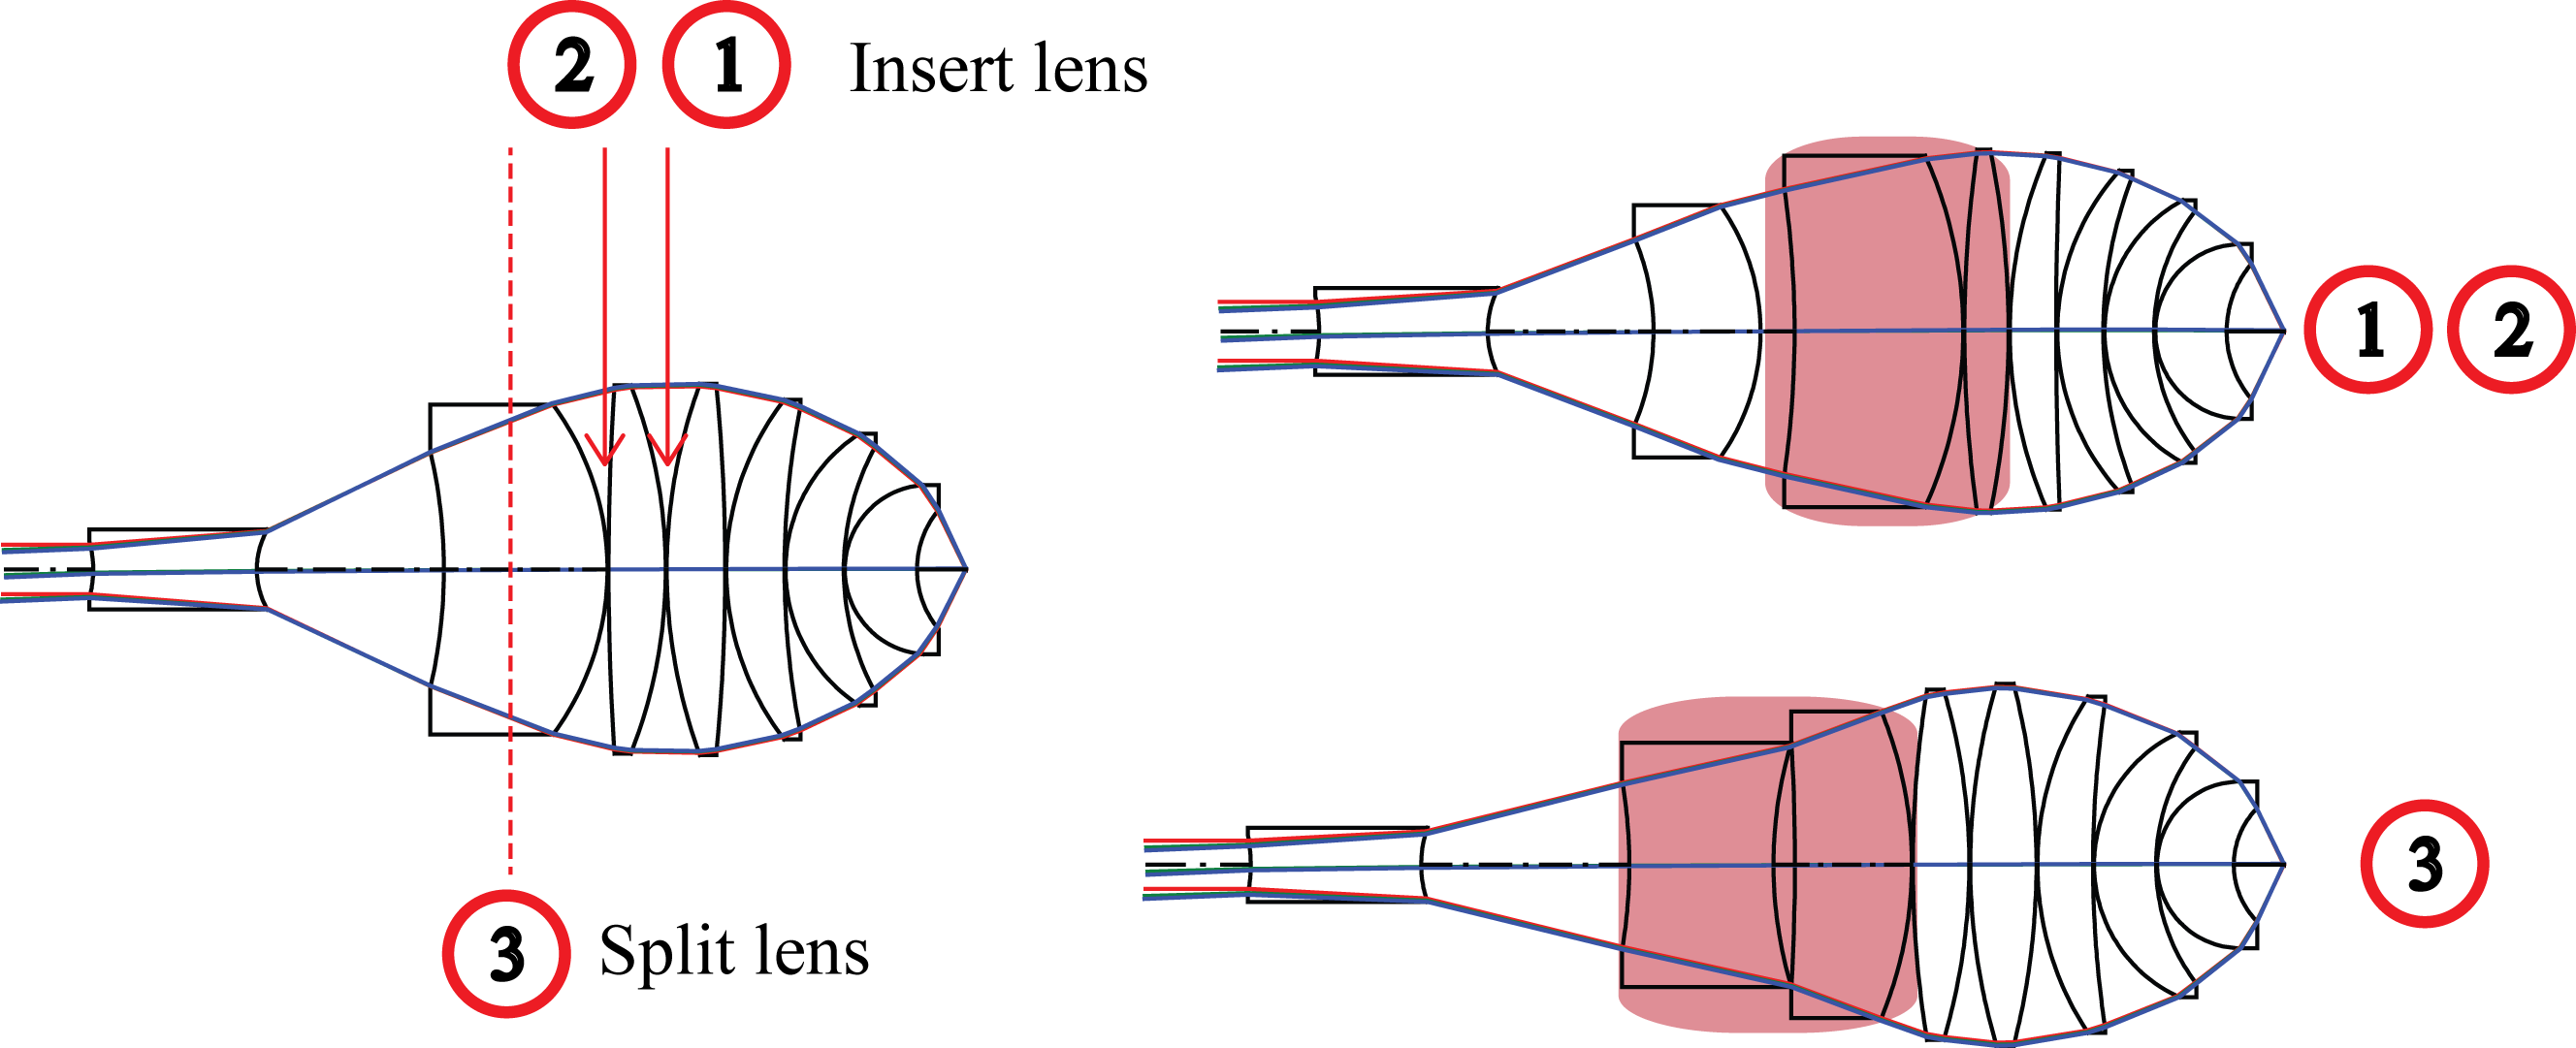
\includegraphics[width=0.6\textwidth]{chapter-4/figures/vollrathWDTrad.png}
    \caption{Introducing structural change in the traditional way to improve the performance of the system. Insertions at position \textcircled{\scriptsize{1}} and \textcircled{\scriptsize{2}} result in the same solution. }
    \label{fig: vollrathWDTrad}
\end{figure}
SPC scans are applied at the same positions where a lens is added or split. The result is shown in Figure \ref{fig: vollrathWDSPC}. From three operations of SPC, ten systems were obtained. The performance of these 10 systems is listed in Table \ref{table: vollrathWDcase}. Out of the ten systems, six have low wavefront RMS value and Strehl ratio above 0.8 for both fields. By carefully examing the system plots in Figure \ref{fig: vollrathWDSPC}, it is seen that some systems have similar system shapes. For example, systems \circled{1}B, \circled{2}B, and \circled{3}B have very close bending for each lens element. The differences among the three are in the lens thickness and air space variations. System \circled{2}A and system \circled{3}A also are very similar. When compared with the results from the conventional approach, system \circled{3}D in Figure \ref{fig: vollrathWDSPC} and system \circled{3} in Figure \ref{fig: vollrathWDTrad} are comparable solutions (especially with respect to the front group on the right). Both systems have Strehl ratio above 0.9 and have close wavefront RMS (39 and 41 $m\lambda$, where SPC constructed one has slightly better performance).

In this example where the working distance is increased, with the conventional approach, two systems were obtained with three operations. One out of three (33\%) has good performance. Using SPC, ten systems were obtained with the same amount of operations as needed in the traditional approach. Six out of ten (60\%) give satisfactory performance. 

\begin{figure}[h!]
    \centering
    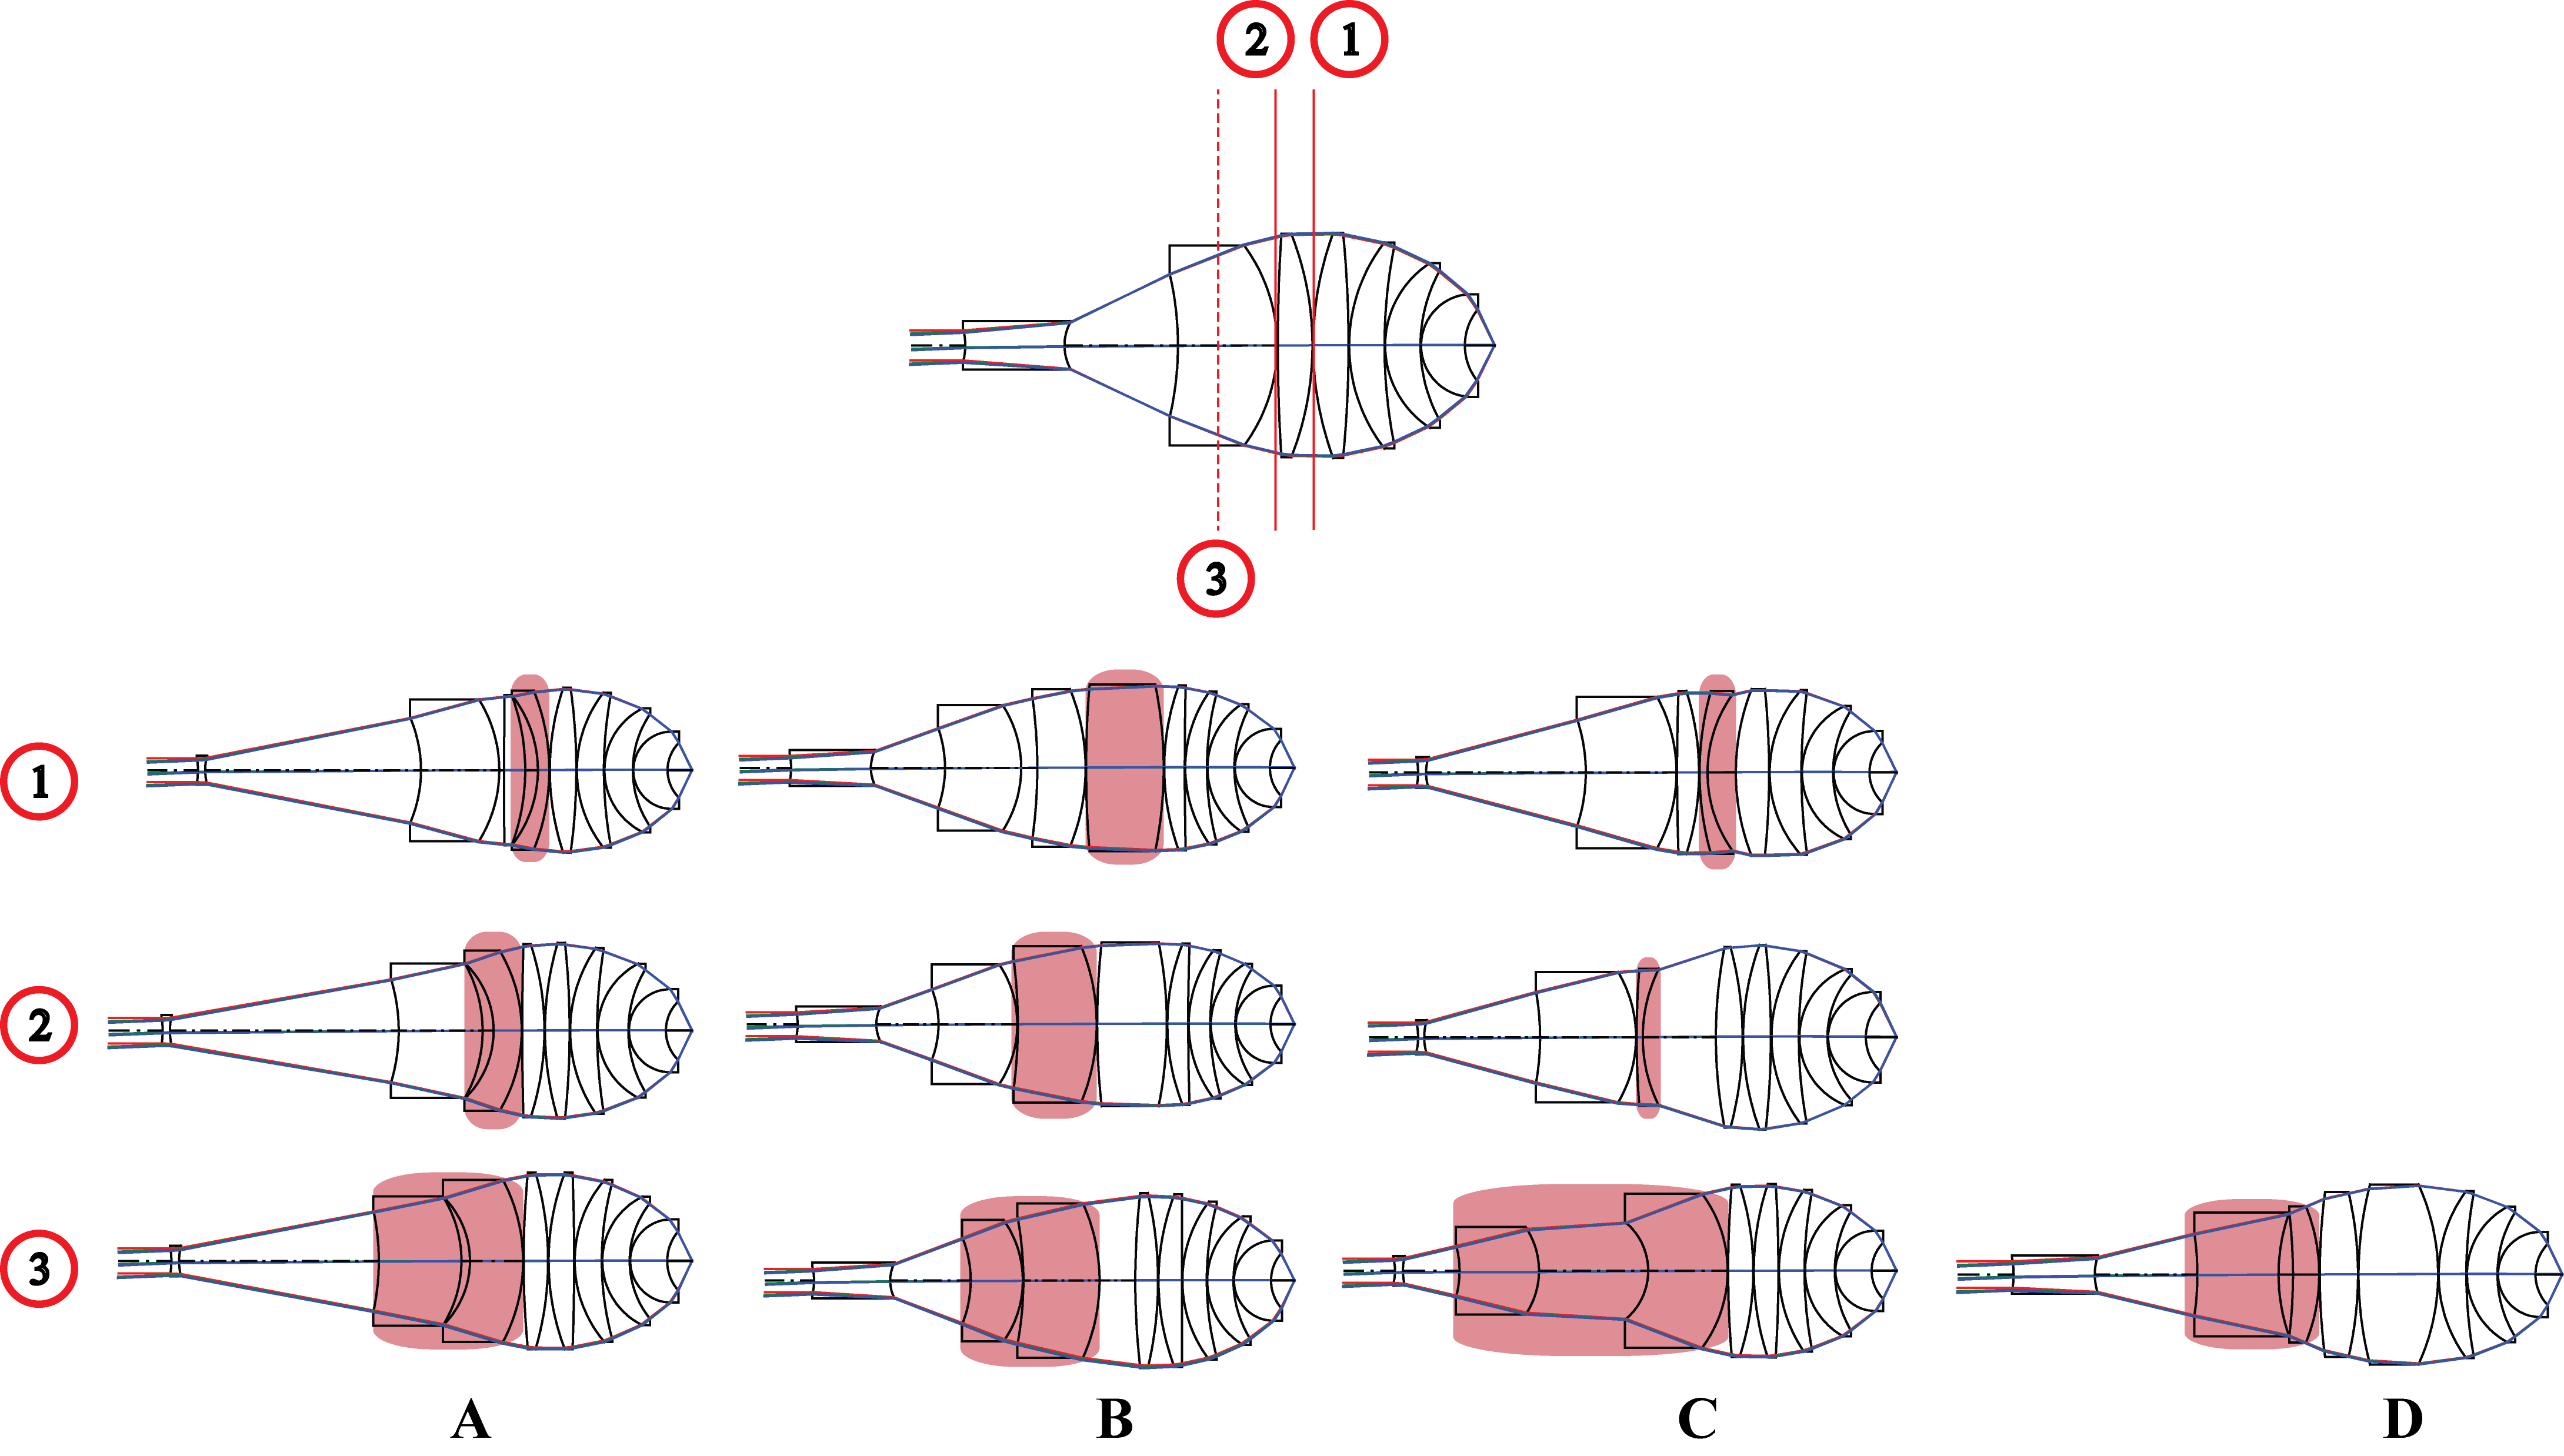
\includegraphics[width=\textwidth]{chapter-4/figures/vollrathWDSPC.png}
    \caption{Systems obtained using three SPC scans performed at the marked locations. Solid lines (\textcircled{\scriptsize{1}} and \textcircled{\scriptsize{2}}) indicate insertion of glass null-element. Dashed line (\textcircled{\scriptsize{3}}) indicates insertion of air null-element. In total, ten systems were obtained. The modified parts are highlighted.}
    \label{fig: vollrathWDSPC}
\end{figure}

\setlength{\arrayrulewidth}{.5mm}
\setlength{\tabcolsep}{18pt}
\renewcommand{\arraystretch}{1.2}
\begin{table}[h!]
    \centering
    \captionsetup{justification=centering}
    \caption{System performance for the systems shown in Figure \ref{fig: vollrathWDSPC}}
    \label{table: vollrathWDcase}
    \vspace{-1em}
    % \hspace*{-10pt} %adjusting the position of the plot(table) !!!!
    \begin{adjustbox}{max width=\textwidth, center}
    \begin{tabular}{c c c c c}
    \hline 
       & \textbf{1} & \textbf{2} & \textbf{3} & \\ 
     \midrule
    RMS WFR & 55 & 49 & 60 & \multirow{3}{*}{\textbf{A}} \\ 
    SR(0) & 0.952 & 0.976 & 0.946  \\
    SR(0.1) & 0.835 & 0.863 & 0.807  \\
    \midrule
    RMS WFR & 133 & 101 & 179 & \multirow{3}{*}{\textbf{B}} \\ 
    SR(0) & 0.645 & 0.779 & 0.410  \\
    SR(0.1) & 0.309 & 0.511 & 0.131  \\
    \midrule
    RMS WFR & 95 & 43 & 41 & \multirow{3}{*}{\textbf{C}} \\ 
    SR(0) & 0.732 & 0.971 & 0.983  \\
    SR(0.1) & 0.642 & 0.901 & 0.896 \\
    \midrule
    RMS WFR &  & & 39 & \multirow{3}{*}{\textbf{D}} \\ 
    SR(0) &  &  & 0.978 \\
    SR(0.1) &  &  & 0.910 \\
    \hline
    \multicolumn{5}{c}{\textit{\footnotesize{RMS WFR = RMS Wavefront Error (m\textlambda); SR(0) = Strehl Ratio at 0 mm; SR(0.1) = Strehl Ratio at 0.1 mm.}}}\\
    \end{tabular}
    \end{adjustbox}
\end{table}

\newpage

\subsection{Further Consideration when Applying SPC to Complex System}

When working with complex systems, there are some additional factors which have to be considered in order to properly use SPC. These additional factors usually appear because of the increasing complexity of multi-variable optimization and the design approaches in complex lens design. Increased complexity here refers to the increased number of variables used. 

\begin{figure}[h!]
    \centering
    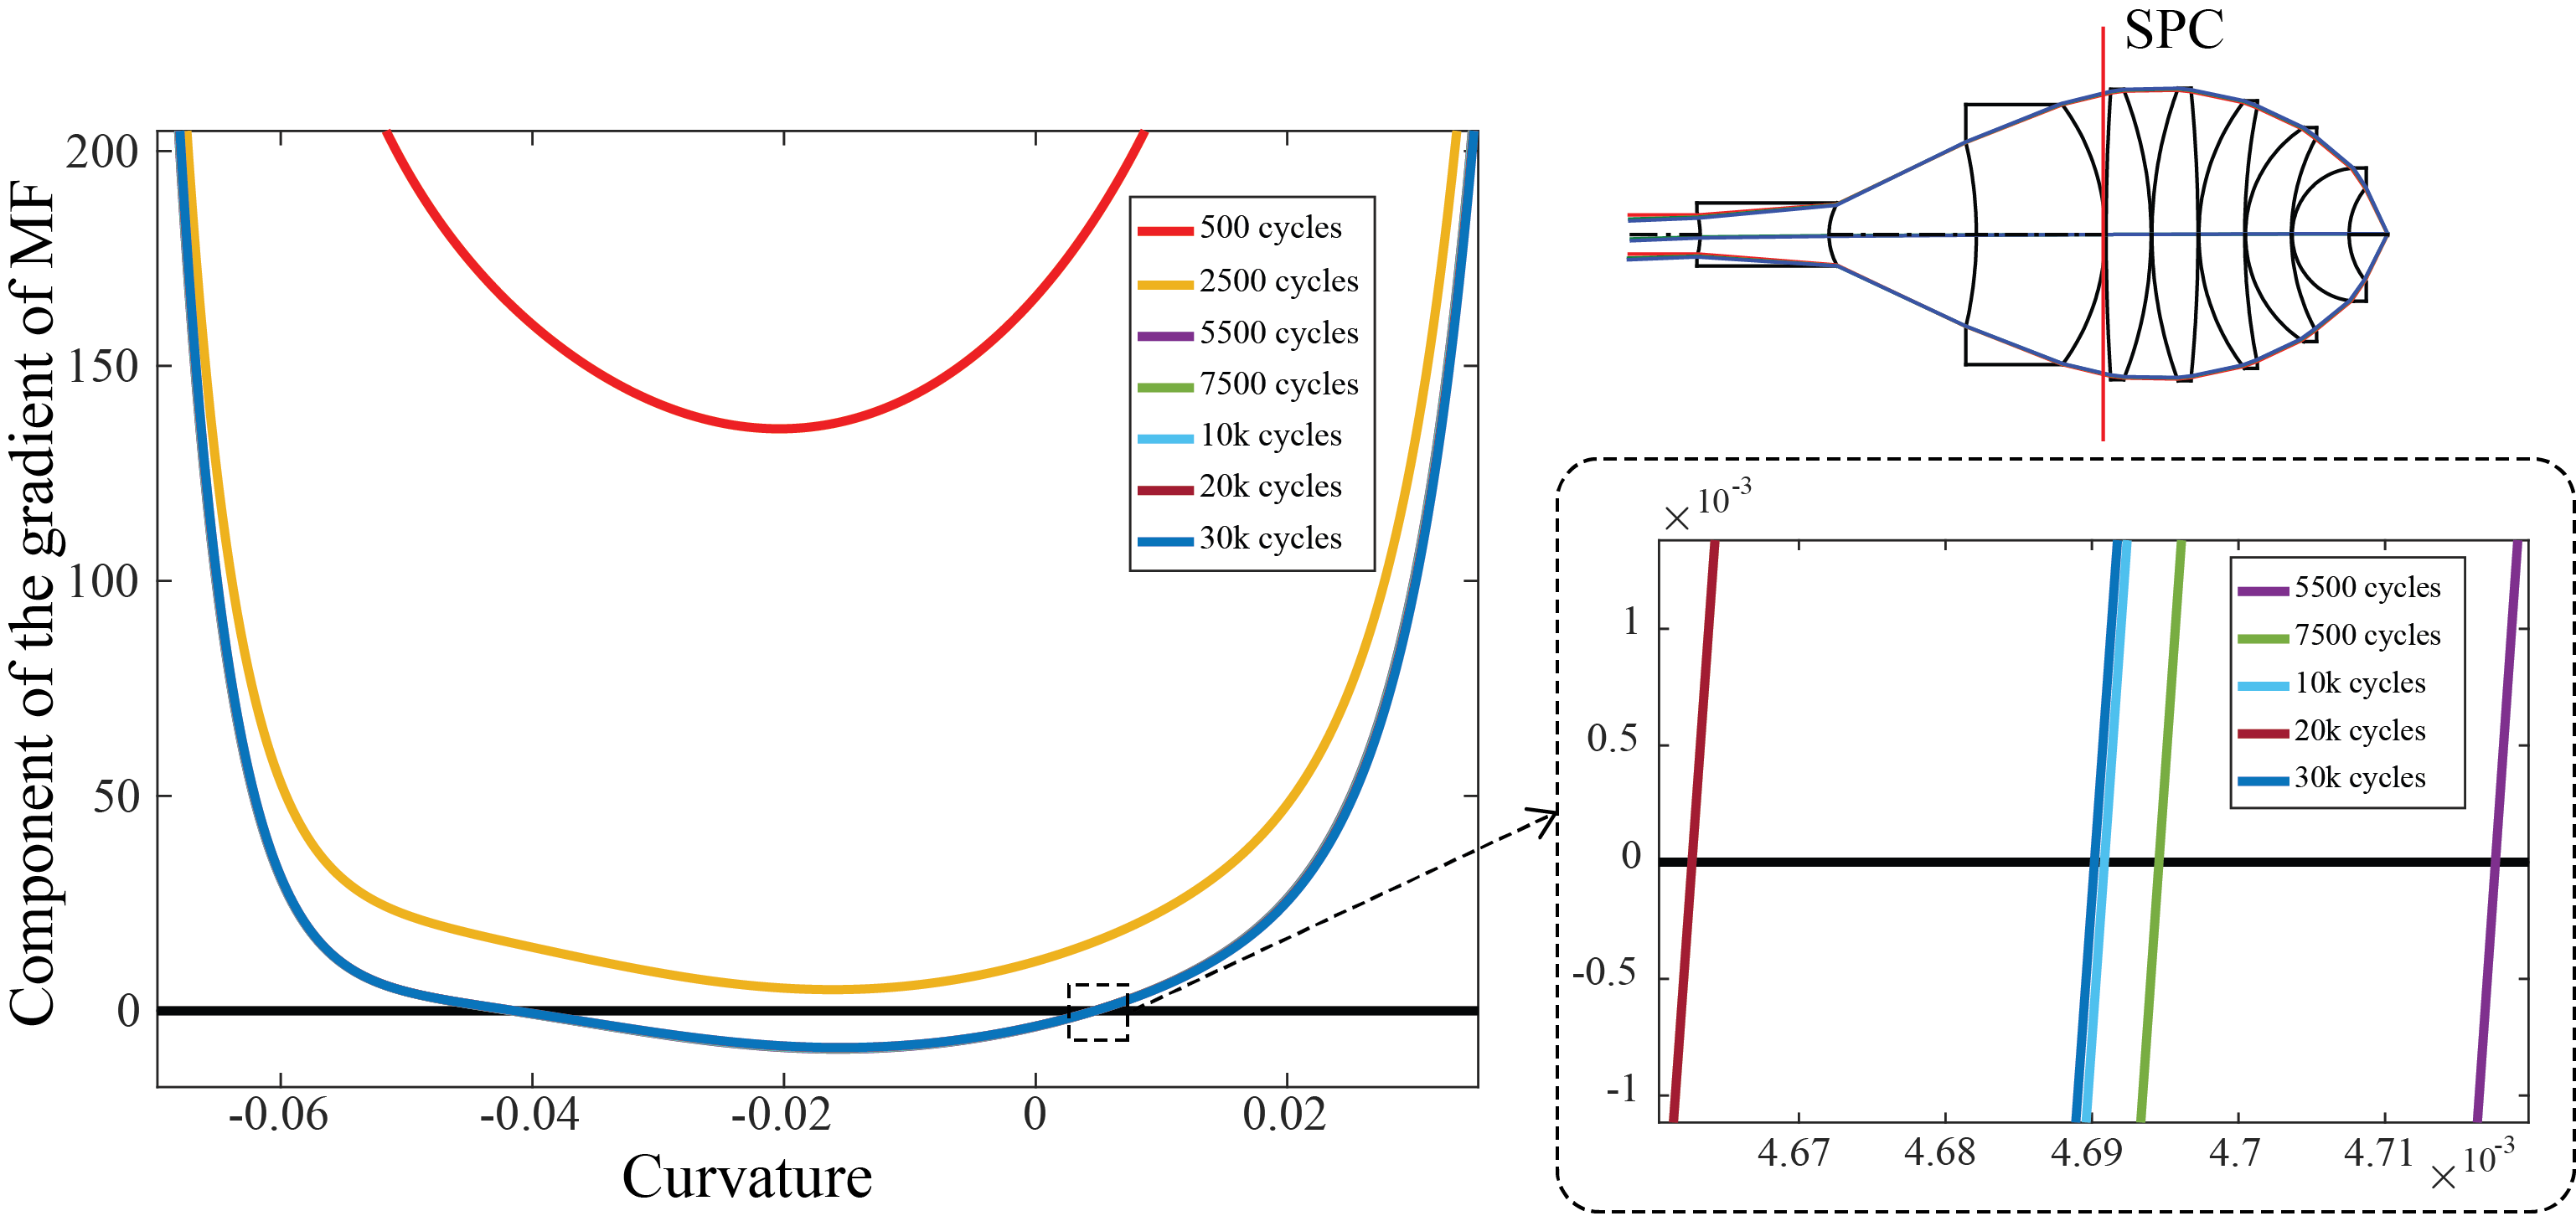
\includegraphics[width=\textwidth]{chapter-4/figures/vollrath_optcyc.png}
    \caption{SPC scan curves at the same position with different numbers of optimization cycles}
    \label{fig: vollrath_optcyc}
\end{figure}

\subsubsection{Quality of the Local Minimum and the SPC Scan Curve}
One of the known issues occurring with complex systems is that often when the number of variables increases, the optimization basin around the local minimum becomes a vast shallow region where absolute convergence can not be achieved and no proper local minimum can be found, even when very large number of optimization cycles are performed \cite{Brixner81}. It is observed that, when the local minima in $N$ dimensional space were not computed accurately, there are problems finding the saddle points in the $N+2$ dimensional space with the SPC method. An example is given for the case where the working distance of the microscope objective is increased. Before proceeding with the SPC scan, the system has to be well-optimized to a local minimum. The merit function is defined by the default transverse ray aberration in CODE V. Two weight constraints were used: an EFL constraint of 2.5 mm and an edge thickness constraint of 2.5 mm on the first surface from the right, both with a weight of 0.01. Fourteen curvatures of the surfaces were used as variables. A threshold for the improvement of the merit function was defined as a criteria to stop the optimization. The threshold was set as $1^{-15}$, which means that when the decrease of the merit function value is less than $1^{-15}$, the optimization will stop. 
 
Without human interference, the optimization for this system ran with 5500 cycles (or optimization iterations), and it took 20 minutes (CPU: Dual-core 3.20GHz) to finish. This implies that there must be a very shallow region around the local minimum where the value of the gradient is close to zero. In the practice of lens design, the designer probably will manually stop the optimization before it runs for 5500 cycles. However, Figure \ref{fig: vollrath_optcyc} demonstrates that the decision of when to stop the optimization affects the number of saddle points that are found. The SPC scan was performed on the fourth surface from the left, as shown in Figure \ref{fig: vollrath_optcyc}. In the same figure, different scan curves are plotted with different numbers of optimization cycles applied. Up to 2500 cycles, there is no crossing between the SPC scan curve and the "$0$ " horizontal axis. From 5500 cycles up to 30,000 cycles, the scan curves are closely positioned giving very similar values of the saddle points. From the zoomed plot in Figure \ref{fig: vollrath_optcyc}, the five curves intersecting the horizontal axis are from 0.00466 to 0.00472. The example shows that, to properly perform SPC scan, it is necessary to compute the local minimum very accurately, even if the local optimization may take many more steps than usual. In this case, with insufficient optimization, two saddle points may be missed. Consequently, the three systems in row \circled{2} (the second row) of Figure \ref{fig: vollrathWDSPC} would not be obtained. 

\subsubsection{Choice of Weights and Constraints}
Other aspects which also require attention concerning SPC scans are the choices of constraints and their weights used in the merit function. As explained in Section \ref{Constraints in optical design software}, using weighted function (or penalty function, essentially identical to weighted function) for constraints implementation is compatible with SPC scan. As a result, adding weighted constraints alters the topography of the optimization landscape.  In this section, we explain the choice of constraints and their weights, change the shape of the SPC scan curve significantly. In some cases, the number of obtained saddle points varies for different combinations of constraints and weights. 

In Figure \ref{fig: vollrath_consdif}, the scan curves of two choices of constraints are shown. Case - 1 (the red-coloured line in Figure \ref{fig: vollrath_consdif}) was only with an effective focal length constraint, and Case-2 was using both an effective focal length constraint and an edge thickness constraint. As seen in the figure, the scan curve of Case-1 has six zero-crossings with the horizontal axis, whereas that of Case-2 has only two zero-crossings. 
\begin{figure}[h!]
    \centering
    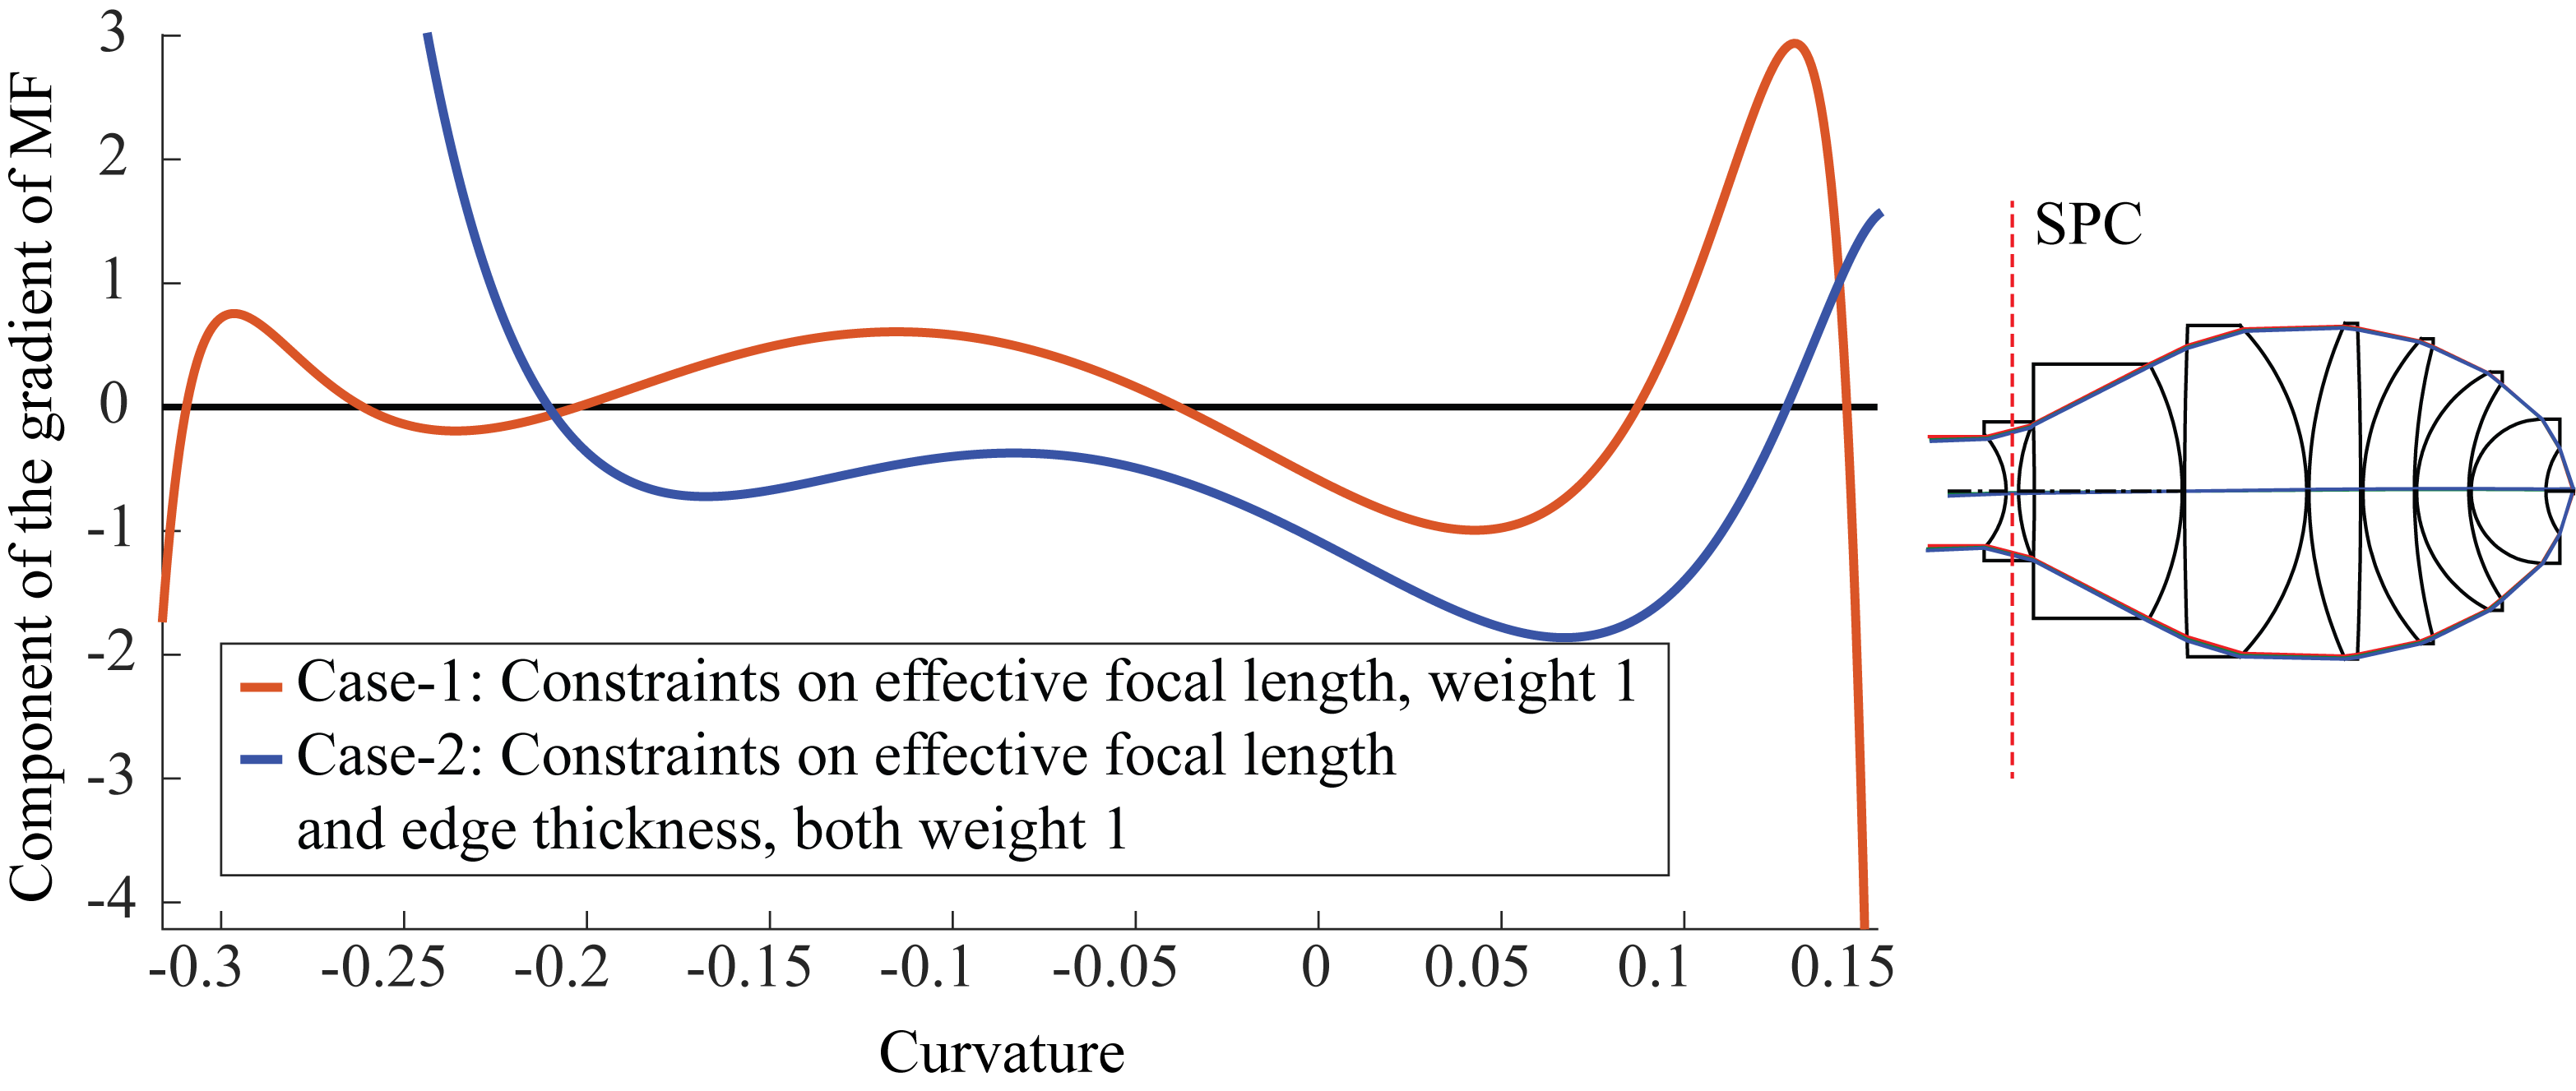
\includegraphics[width=\textwidth]{chapter-4/figures/Vollrath_ConstraintDif.png}
    \caption{Change in the saddle point scan curve when different constraints are applied.}
    \label{fig: vollrath_consdif}
\end{figure}

In practice, the number of local minima is more important than the number of constructed saddle points. For the given example, Case-1 did not include the edge thickness requirement in the merit function. If this requirement is not met, it is necessary to add the constraint on the edge thickness and optimize from the minima acquired in the next step. In Case-2 the two necessary constraints on the EFL and the edge thickness are taken account of from the start, hence, the acquired minima are the final solutions. Design procedure and the obtained local minima are shown for both cases in Figure \ref{fig: vollrath_constr_flow}. For Case-1, seven local minima are acquired from six saddle points. For Case-2, three minima are obtained from two saddle points. Judging by the system shapes, the three minima from Case-2 correspond to the local minima in the set obtained in Case-1. The pairs of corresponding local minima are highlighted with different colours in Figure \ref{fig: vollrath_constr_flow}. It is seen that MA-4 and MB-2, which belong to the same system shape, have very similar merit function values. However, the two pairs MA-1, MB-1 and MA-6, MB-3 have bigger differences in their merit function values. Although the system shapes are similar, due to the complex topography of the design landscape in the case of many variables, the merit function values can be quite different. The same observation was described in \cite{PascalTriplet2009}. 


\begin{figure}[h!]
    \centering
    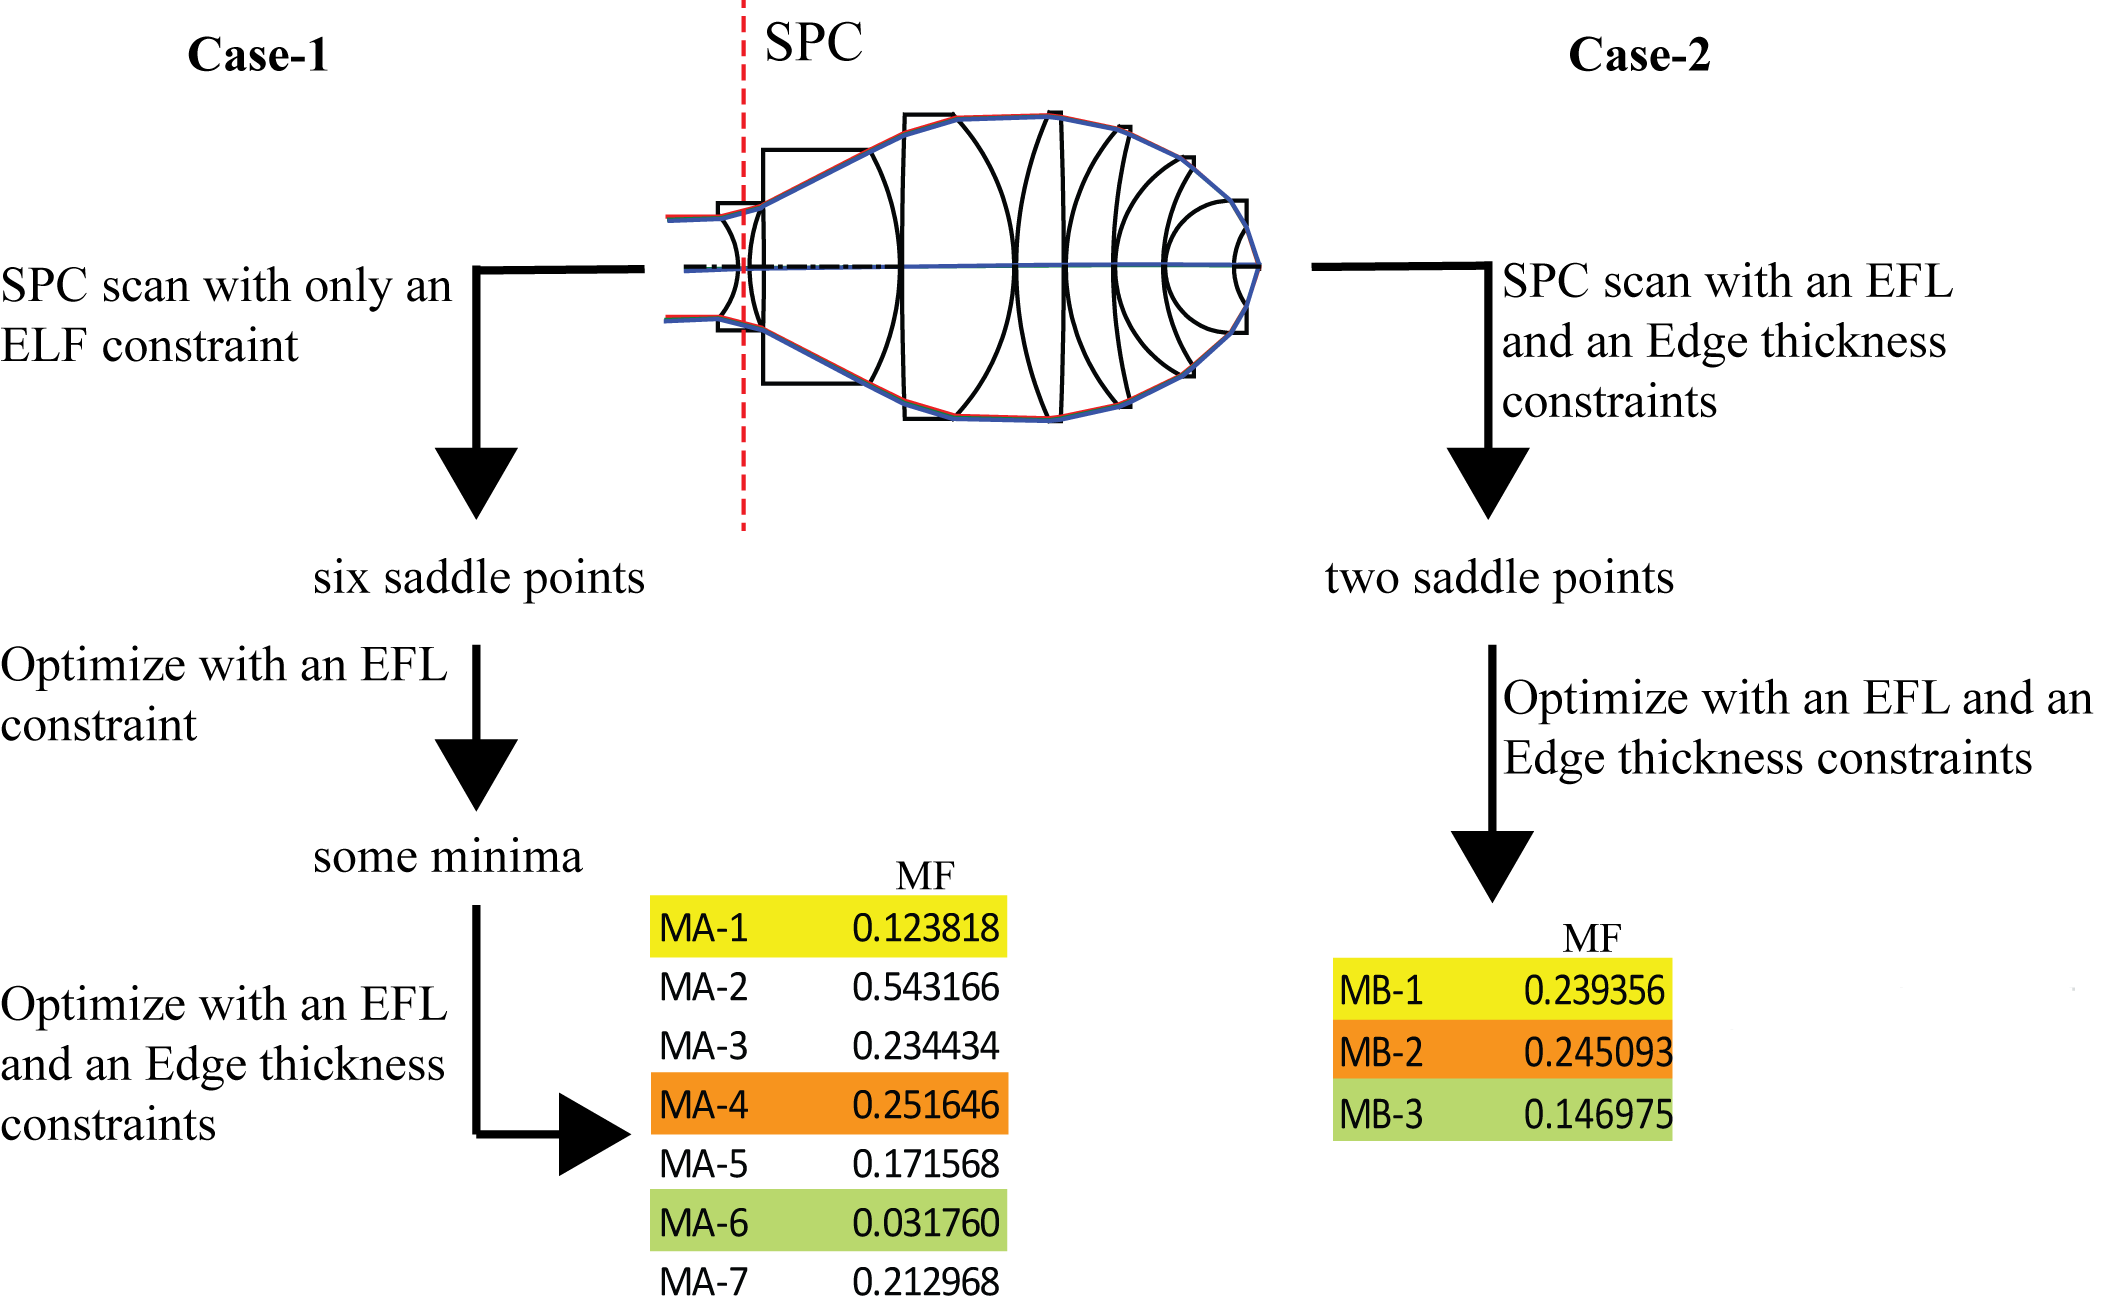
\includegraphics[width=\textwidth]{chapter-4/figures/Vollrath_ConstraintDif_flow.png}
    \caption{Two different design processes leading to different sets of local minima. On the left: saddle point scan with only the EFL constraint, with the edge thickness constraint applied only in the last stage. In total seven minima are obtained. On the right: SPC scan with both EFL and edge thickness constraints incorporated followed by local optimization using both constraints. This led to three local minima. Systems with similar shapes are given the same colour.}
    \label{fig: vollrath_constr_flow}
\end{figure}

In addition to the number of constraints used, the choice of the weight also affects the SPC scan curve. An example is given in Figure \ref{fig: vollrath_wt_change}, where different scan positions are chosen using the same system from the previous example. Only the EFL constraint is applied here with different weight number from 0.001 to 10. In Figure \ref{fig: vollrath_wt_change}, it is shown that when the weight is 0.001 or 10, the SPC scans produce curves that differ from those in the other three cases. Weight 0.001 gives four saddle points, weight 10 gives two saddle points, and the other three cases give three saddle points. The target value of the EFL is 2.50 mm. When a weight of 0.001 is used, the optimized system has an EFL of 2.65 mm. For a weight of 0.01, the EFL is stabilized around 2.53 mm. When the weight is larger than 0.1, the optimized system has an intended EFL of 2.50 mm. 

According to the derivation of the special case of SPC \cite{BociortSPCSexplained}, when the space between the constructed surface and another optical surface is zero (or close to zero), a saddle point can be found with the curvatures of the constructed surface identical (or similar) to that optical surface. In this example, when the weight is 0.01, 0.1 and 1, the most left and most right saddle points represent the special case saddle points. However, when the weight is too big or too small, the design landscape is altered in a way that the special case of saddle point cannot be obtained via the scan (weight 10 case missed the left one). One of the hypotheses is that there are some numerical inaccuracy when computing the local minima and saddle points with these extreme weights. More investigations are needed to understand these situations. Based on the observations in this example, for practicing the SPC, we would suggest to avoid using extreme weight values. 

From the two examples, it is seen that the way to implement the constraints affects the number of saddle points acquired from SPC. This will lead to differences in the obtained minima. Regarding the constraints applied, the example shows that starting with a simple constraint generates more saddle points than applying several constraints at the same time. It is consistent with the design rule that constraints are usually added progressively. If all constraints are added at the same time, using the Lagrange Multiplier method adds multiple new variables to the optimization problem, therefore can generate more local minima and make the global optimization more difficult. When using the weight function, there is lack of systematic knowledge on how to adjust multiple weights in one merit function. Constraints that are not massively violated should not be included in the SPC scan, but should be applied only on the resulting minima. We recommend avoiding extreme values of weight when using SPC with a merit function containing weight constraints. In general, the weights should be adapted during the design process, depending on the problem. When applying SPC, it is necessary to keep the weights the same during the application of SPC and the following local optimizations. After obtaining the local minima, the weights can be adapted when the design process is continued. 

\begin{figure}[h!]
    \centering
    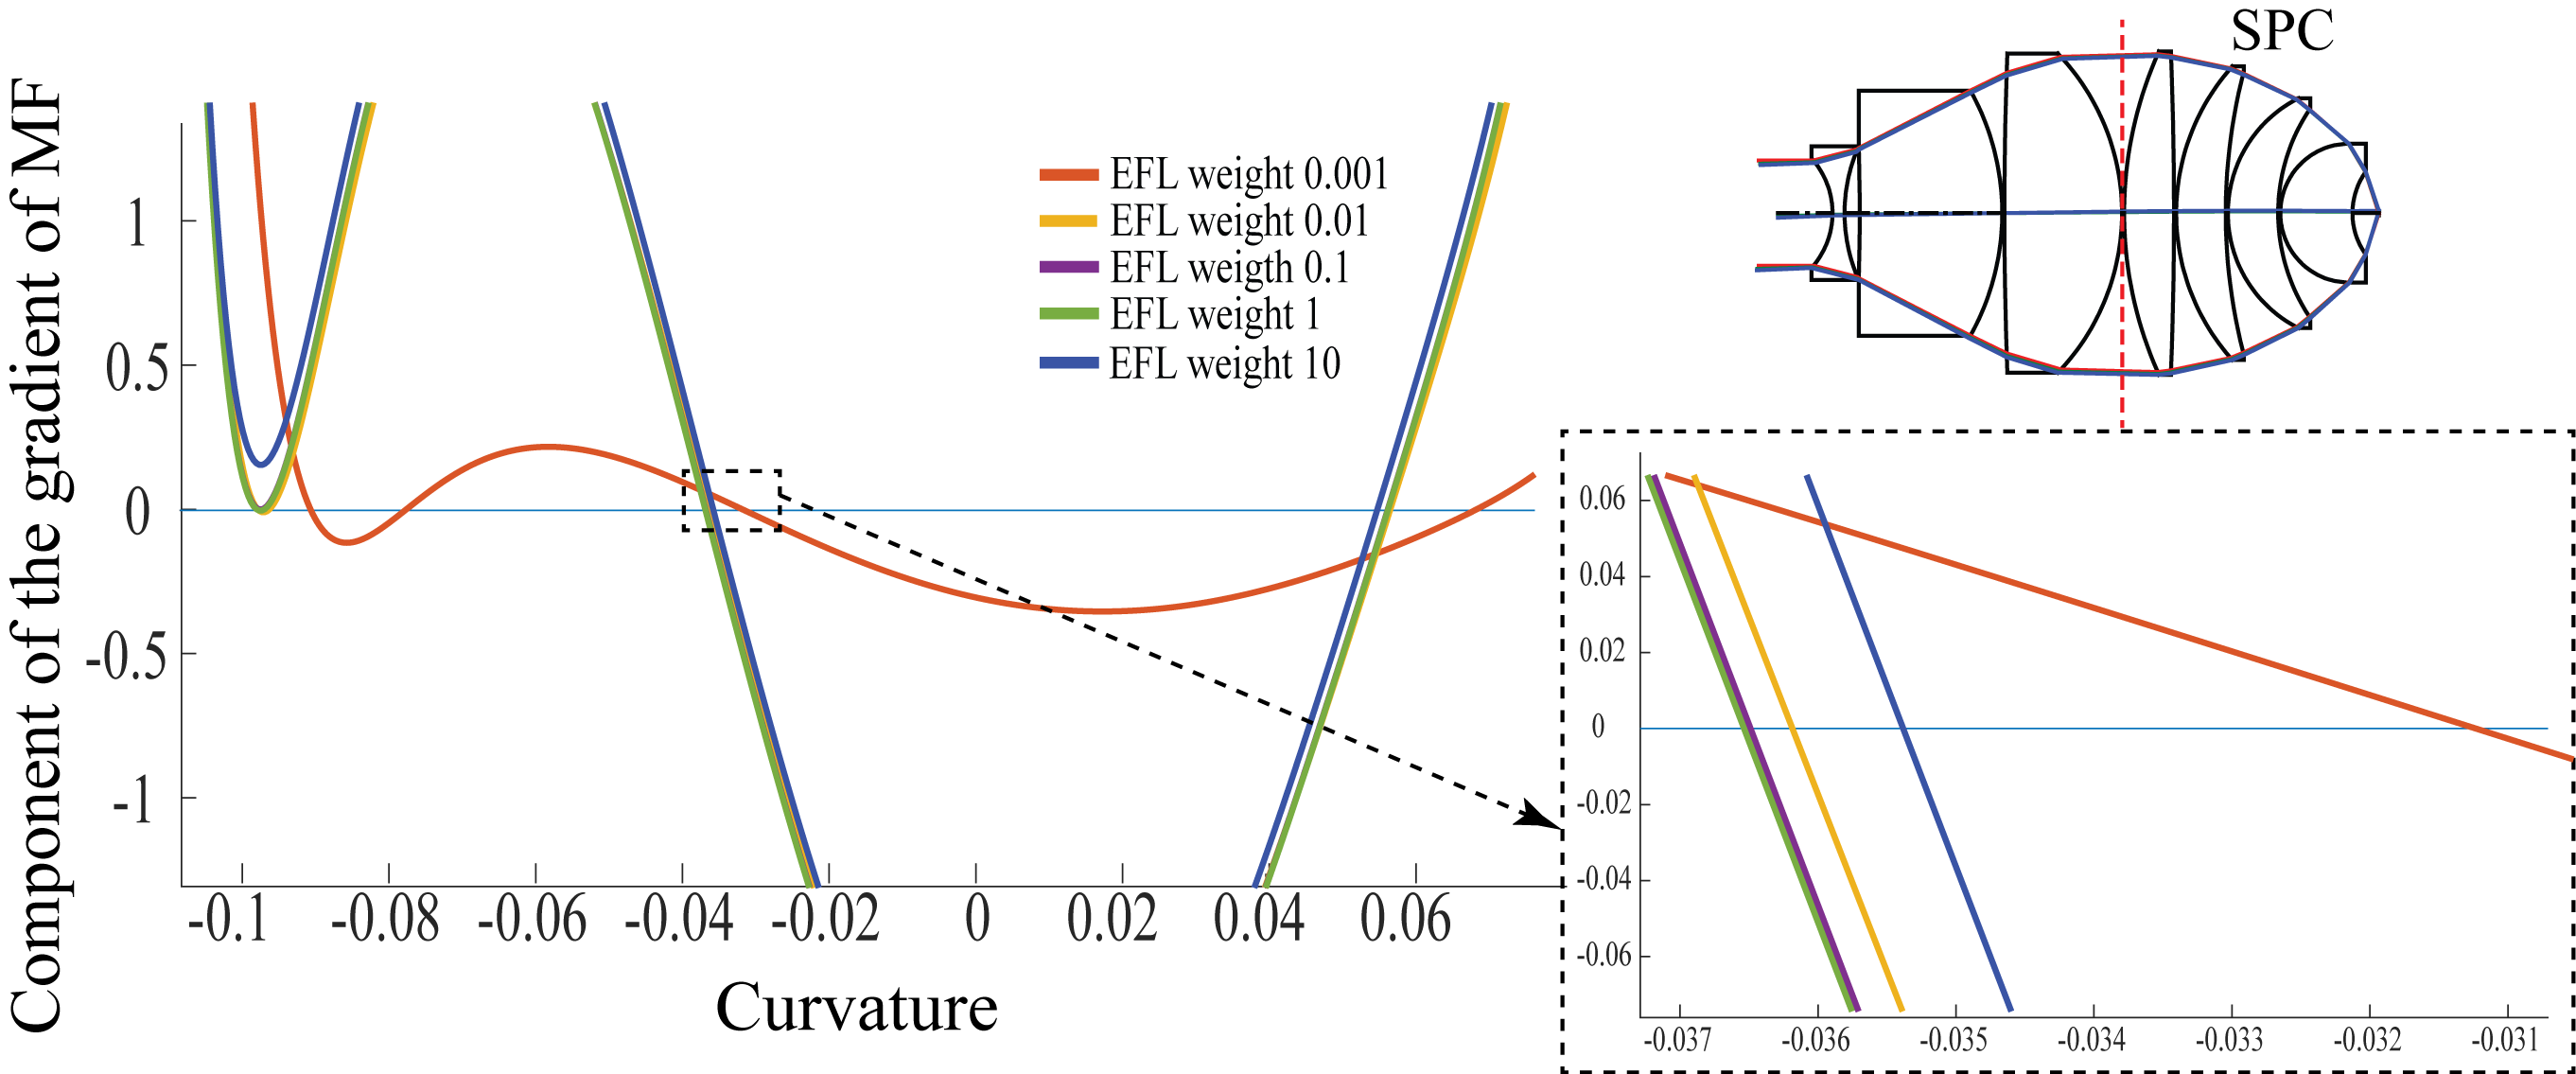
\includegraphics[width=\textwidth]{chapter-4/figures/Vollrath_wt_change.png}
    \caption{Change in the saddle point scan curve when different constraint weights are applied.}
    \label{fig: vollrath_wt_change}
\end{figure}

\newpage
\section{Applying SPC to a Photo-Lithographic Objective}
Lithographic systems represent one of the most sophisticated types of optical systems nowadays. With an imaging objective consisting of more than twenty lens elements, nanometer resolution has to be realized. These systems are used in the semiconductor industry to produce integrated chips \cite{Matsuyama2006_LithoHis}, which boost all kinds of technology advances in the 21st century. 

For these kinds of complicated optical systems with a large number of variables, the number of possible solutions increases drastically. These systems suffer more easily from ray failures. Varying variables in the system can easily cause failures in ray tracing. Normally, a new design starts from an existing one, where the system specification is close to the design requirement. The system is then modified by the designer based on certain design guidelines \cite{LivshitsQA2013}\cite{Shafer1995_moreless}\cite{Cao2017_GroupDesign} or his/her own experience. Trial and error always evolves before obtaining a good solution. 

A Deep Ultra Violet (DUV) lens from an existing patent \cite{patentZeissDUV} is selected. We choose the design from the embodiment described in Figure 5 of this patent. The system parameters are given in Table 5 in the patent. We use this DUV objective as an example to demonstrate how SPC can be applied in a complex case. The DUV objective is designed to work at 193 nm wavelength. The numerical aperture is 0.85, the image height is 14.02 mm and the magnification is -0.25. The system is optimized for distortion and telecentricity. The wavefront RMS error is 3.26 $m\lambda$. The objective consists of twenty-three lens elements, where eight surfaces are aspheric. The system plot is presented in Figure \ref{fig: litho_DUV_plot}. 
\begin{figure}[h!]
    \centering
    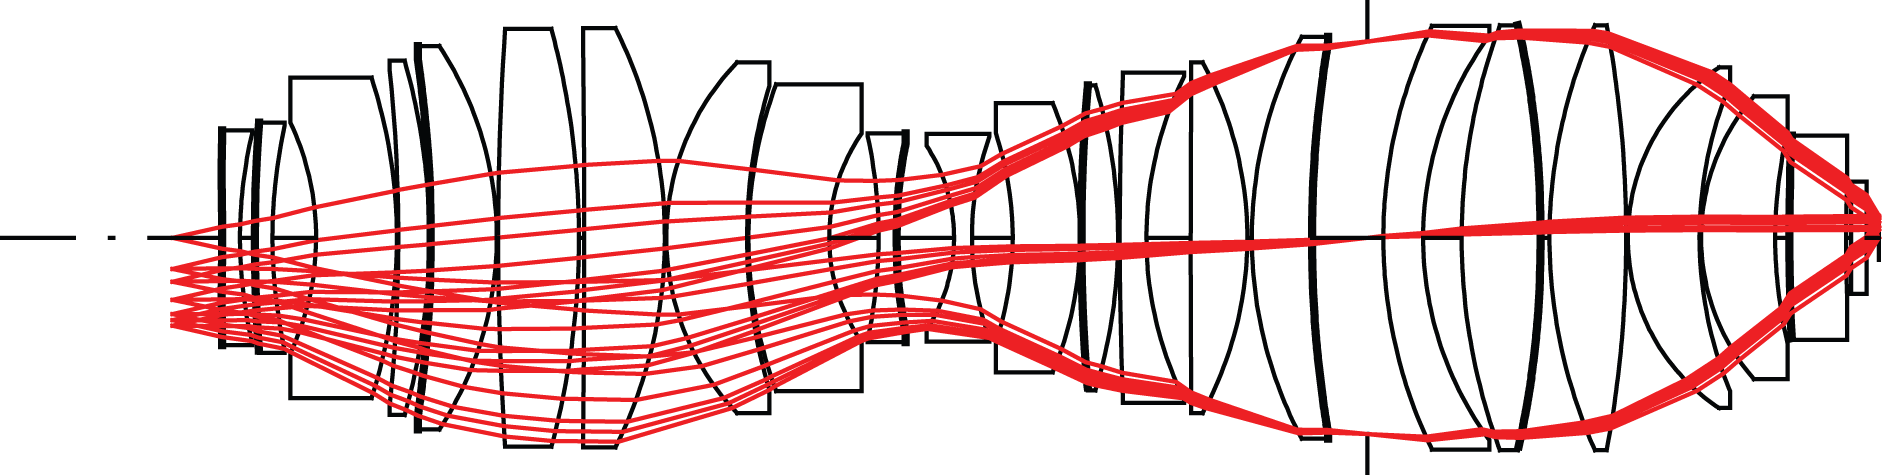
\includegraphics[width=\textwidth]{chapter-4/figures/Litho_DUV_plot.png}
    \caption{DUV objective lens from \cite{patentZeissDUV}. It consists of, in total, twenty-three lens elements. Eight surfaces are aspheric surfaces marked by thickened line.}
    \label{fig: litho_DUV_plot}
\end{figure}

This objective has been previously studied with the special version of SPC. In the special version, no curvature scan is used. The designer decides where to insert the null-element. This is always done on an existing surface. A saddle point system is directly obtained by the way the null element is inserted \cite{BociortSPCSexplained}. Two new solutions can be obtained by optimizing from the saddle point. In the study of Marinescu\cite{OanaThesis2006}\cite{OanaOEngPart2}, examples are given to use the special version of SPC to add lenses to the original system to obtain different local minima. Afterwards, other lenses are chosen to be deleted. In this way, the system maintains similar performance with a smaller number of optical elements. However, the strategy for where to add or extract the lenses is not explained in detail. This question remains unanswered by our research, and it makes the design of large systems more complicated. Marinescu's method has two steps: 1) choose the place to add a lens with SPC; 2) choose lenses to be extracted. The design process is a combination of SPC and conventional methods. The designer needs to make the decision twice on where to add and extract the lens. In the following examples, we will show that with SPC, the designer only needs to decide once where to perform SPC to achieve performance improvement. 

The sixth lens (from the left) is chosen to be replaced using SPC following the example in Marinescu's thesis (where she chose to add a null-element next to it). The first step was to remove the chosen lens by gradually reducing the thickness of the lens while optimizing the system, at the same time to keep the system staying in the same basin of attraction. Once the thickness is reduced to zero, constraints are applied to make the element a meniscus null-element (equal curvature with zero-thickness). In this way, the element could be removed without affecting the system. In practise, the element does not need to be physically removed, since the next step is to perform an SPC scan at the same location. 

As demonstrated in the previous section, the choice of constraints in the merit function may affect the obtained result. The recommendation is to start with a relative simple merit function. The complexity of the merit function can be increased after the SPC process. A default unconstrained merit function based on wavefront aberration \footnote{In CODE V, the merit function is based on wavefront variance. It comes from the weighted combination of the optical path difference (OPD) and the X and Y wavefront slope values.} is used for the phase of the SPC scan: the variables used are only the curvatures of the spherical surfaces (thirty six variables, the last element is a plane-parallel plate). Since the air spaces and lens thicknesses are not varied and the system is already very "tight", an unconstrained optimization does not drastically change the system. With the default wavefront aberration merit function, the original system has a merit function value of 0.002915, and a wavefront aberration of 3.26 $m\lambda$. After unconstrained optimization, the merit function value becomes 0.002391, and the wavefront aberration increases to 3.53 $m\lambda$. The merit function is calculated assuming that the best focus is determined by the paraxial calculation (ideal focus plane). The wavefront aberration is given by the wavefront analysis in CODE V, which traces the real rays and determines best focus plane using the real rays. Therefore, due to the different choices of the focal planes, a decreased merit function can bring an increased wavefront aberration. The computation technique used in the merit function is aimed for facilitating the optimization. When the sixth lens element was extracted, the merit function deteriorated to 0.013822, and the wavefront aberration increased to 12.39 m\textlambda.

Performing an SPC scan at the position where the sixth lens is extracted, yielded six saddle points. These six saddle points lead to twelve minima with a zero-thickness element. After increasing the thickness, the twelve systems converge into four solutions. The reason for the convergence of the solutions is that when the thicknesses increase, local minima can encounter ray failure or merge with other local minima. An example of ray failure caused by thickness increase is explained in Figure \ref{fig:thickness_increase}. In Figure \ref{fig: litho_step1_2}, the first two steps of performing an SPC scan on the lithographic objective are illustrated.

\begin{figure}[h!]
    \centering
    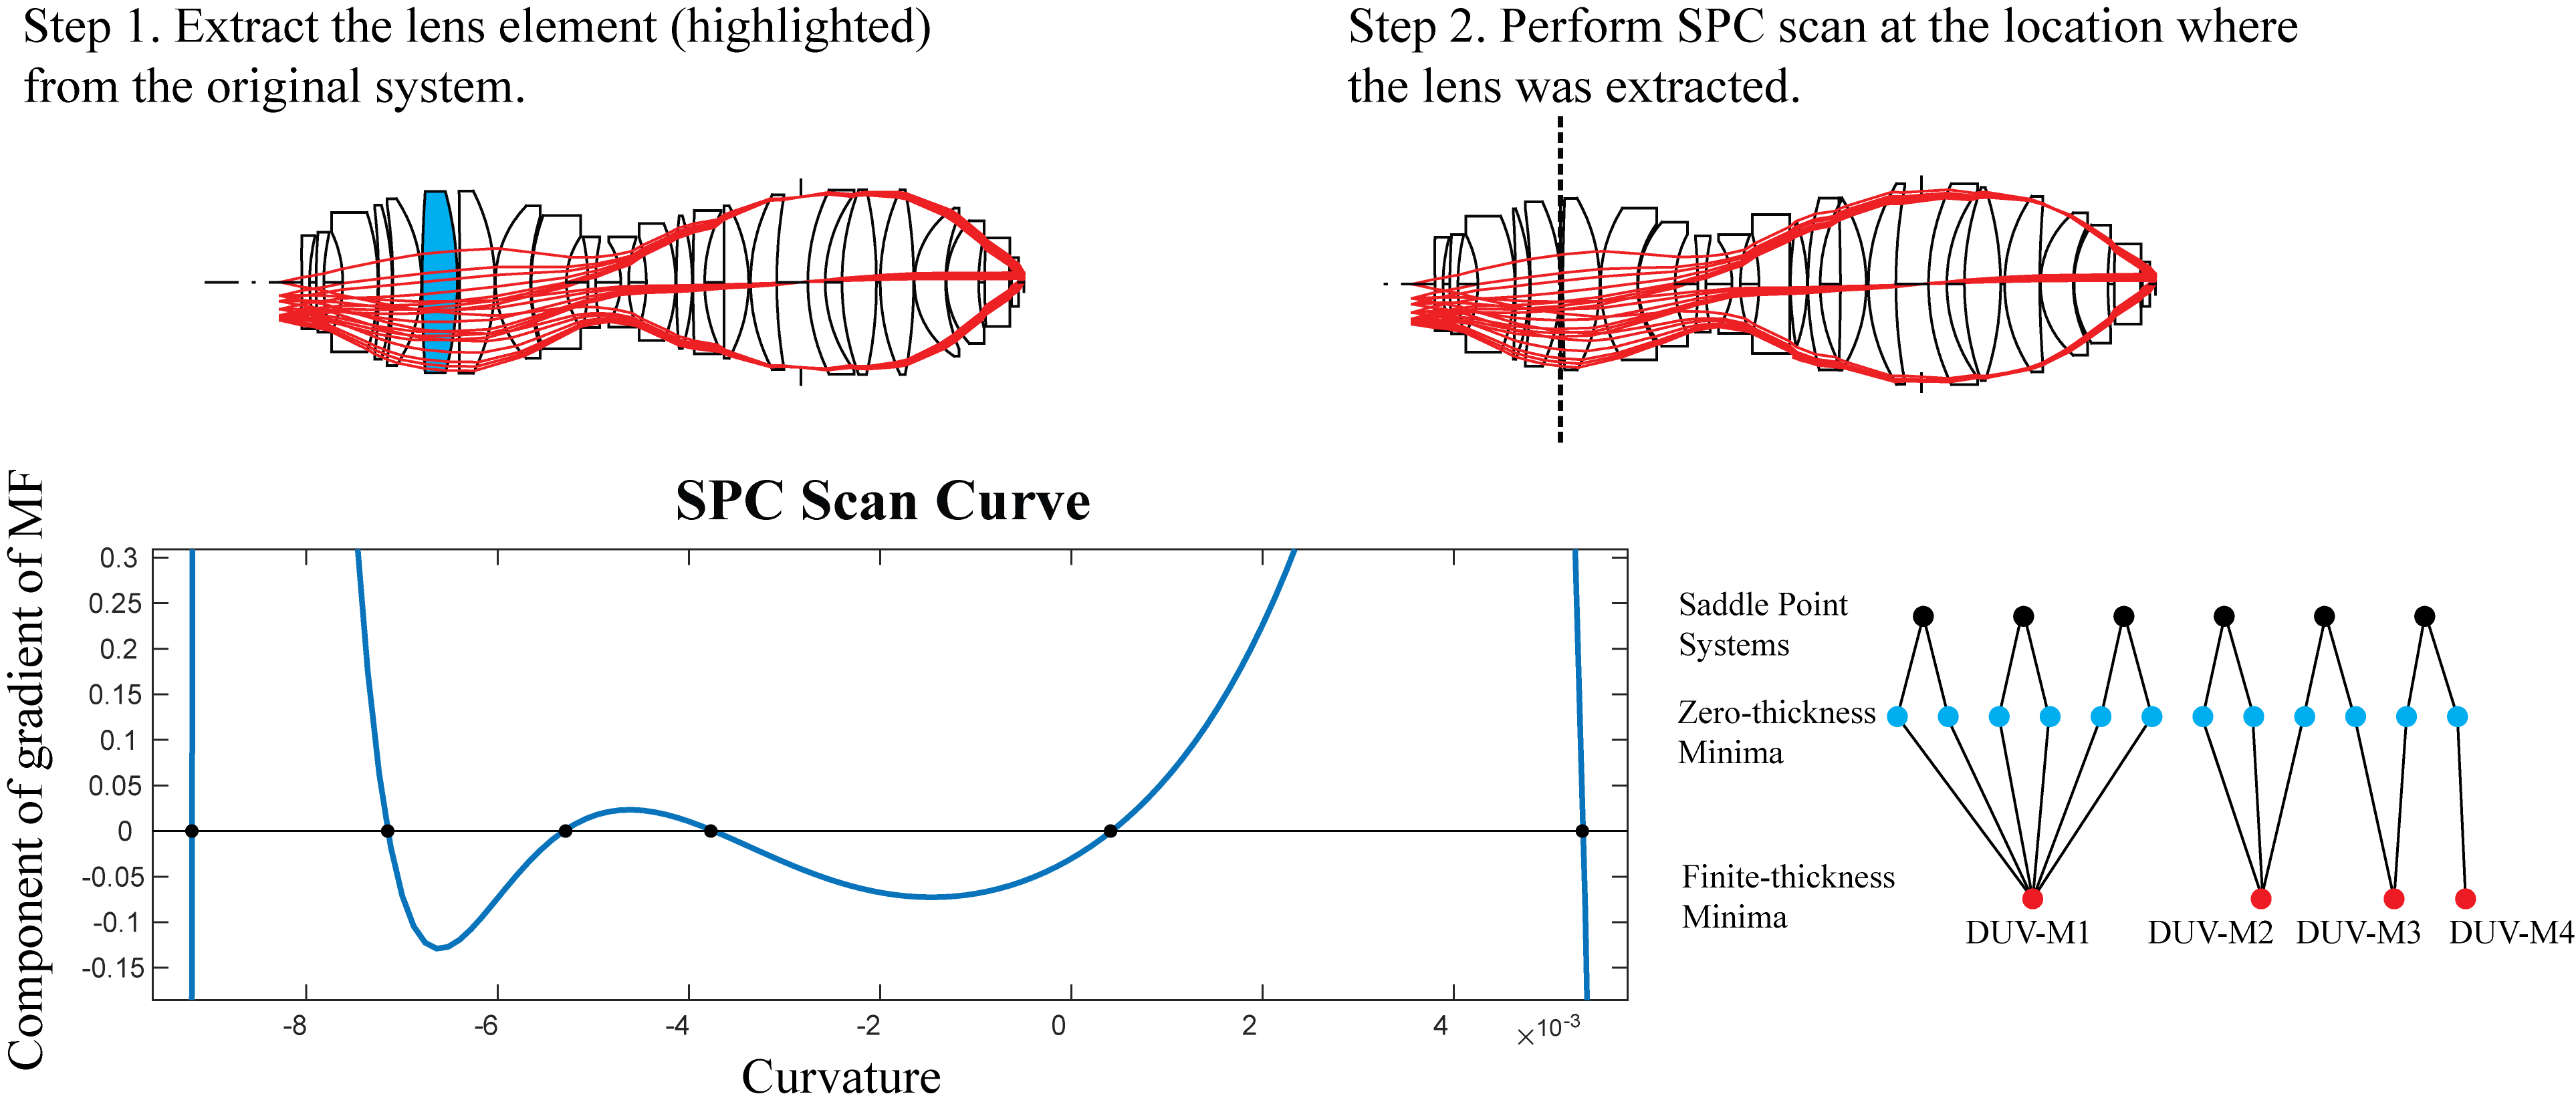
\includegraphics[width=\textwidth]{chapter-4/figures/Litho_Step1_2.png}
    \caption{Step 1, Extract the selected element (highlighted); Step 2, Perform SPC at the location of the extraction (dashed line location). With the SPC scan, six saddle points were obtained which led to four local minima. }
    \label{fig: litho_step1_2}
\end{figure}

The system plots of the four new systems are shown on the left of Figure \ref{fig: litho_Step3}. The extracted and then constructed lens elements are highlighted. It is observed that the new solutions mostly differ from each other in the lenses close to the position of extraction and where the SPC scan is performed. By comparing the systems, we see that the highlighted lens and its neighbouring lens differ in the lens bending between different systems. For example, DUV-M1 has meniscus - meniscus - biconvex around the highlighted lens and DUV-M4 has meniscus - biconvex - meniscus around the highlighted lens. It is also worth noticing that there is no system identical to the original system at the top row of Figure \ref{fig: litho_Step3}. The constructed lens of DUV-M4 shows similar bending shape as the original system, however, the neighbouring right element has a meniscus shape which is different from the plano-convex shape in the original system. One can not expect to find a system that is identical to the original system because the solutions are obtained by optimization without constraints. The next step (Step 3) as shown in Figure \ref{fig: litho_Step3} is to add constraints to the merit function and minutely optimize every solution obtained from the SPC scan. Constraints like magnification, distortion control and edge thickness etc. were added to the original merit function. Weights and number of constraints were tailored for each system in order to reach a solution which has good performance as while as fulfill the constraints. Extra variables such as aspheric coefficients, air spaces and lens thicknesses were also used in the last stage. The corresponding solutions are listed on the right side of Figure \ref{fig: litho_Step3} as DUV M1' - M4'. Judging from the system plots, it is seen that most of the differences between the systems are still localized around the constructed element. Compared to the previous stage, the major change of the further optimized solutions are the thicknesses of the lenses and the air spaces between them. This implies that in the fine tuning optimization stage, the system stays in the same basin of attraction when the curvature variables are varied.


\begin{figure}[h!]
    \centering
    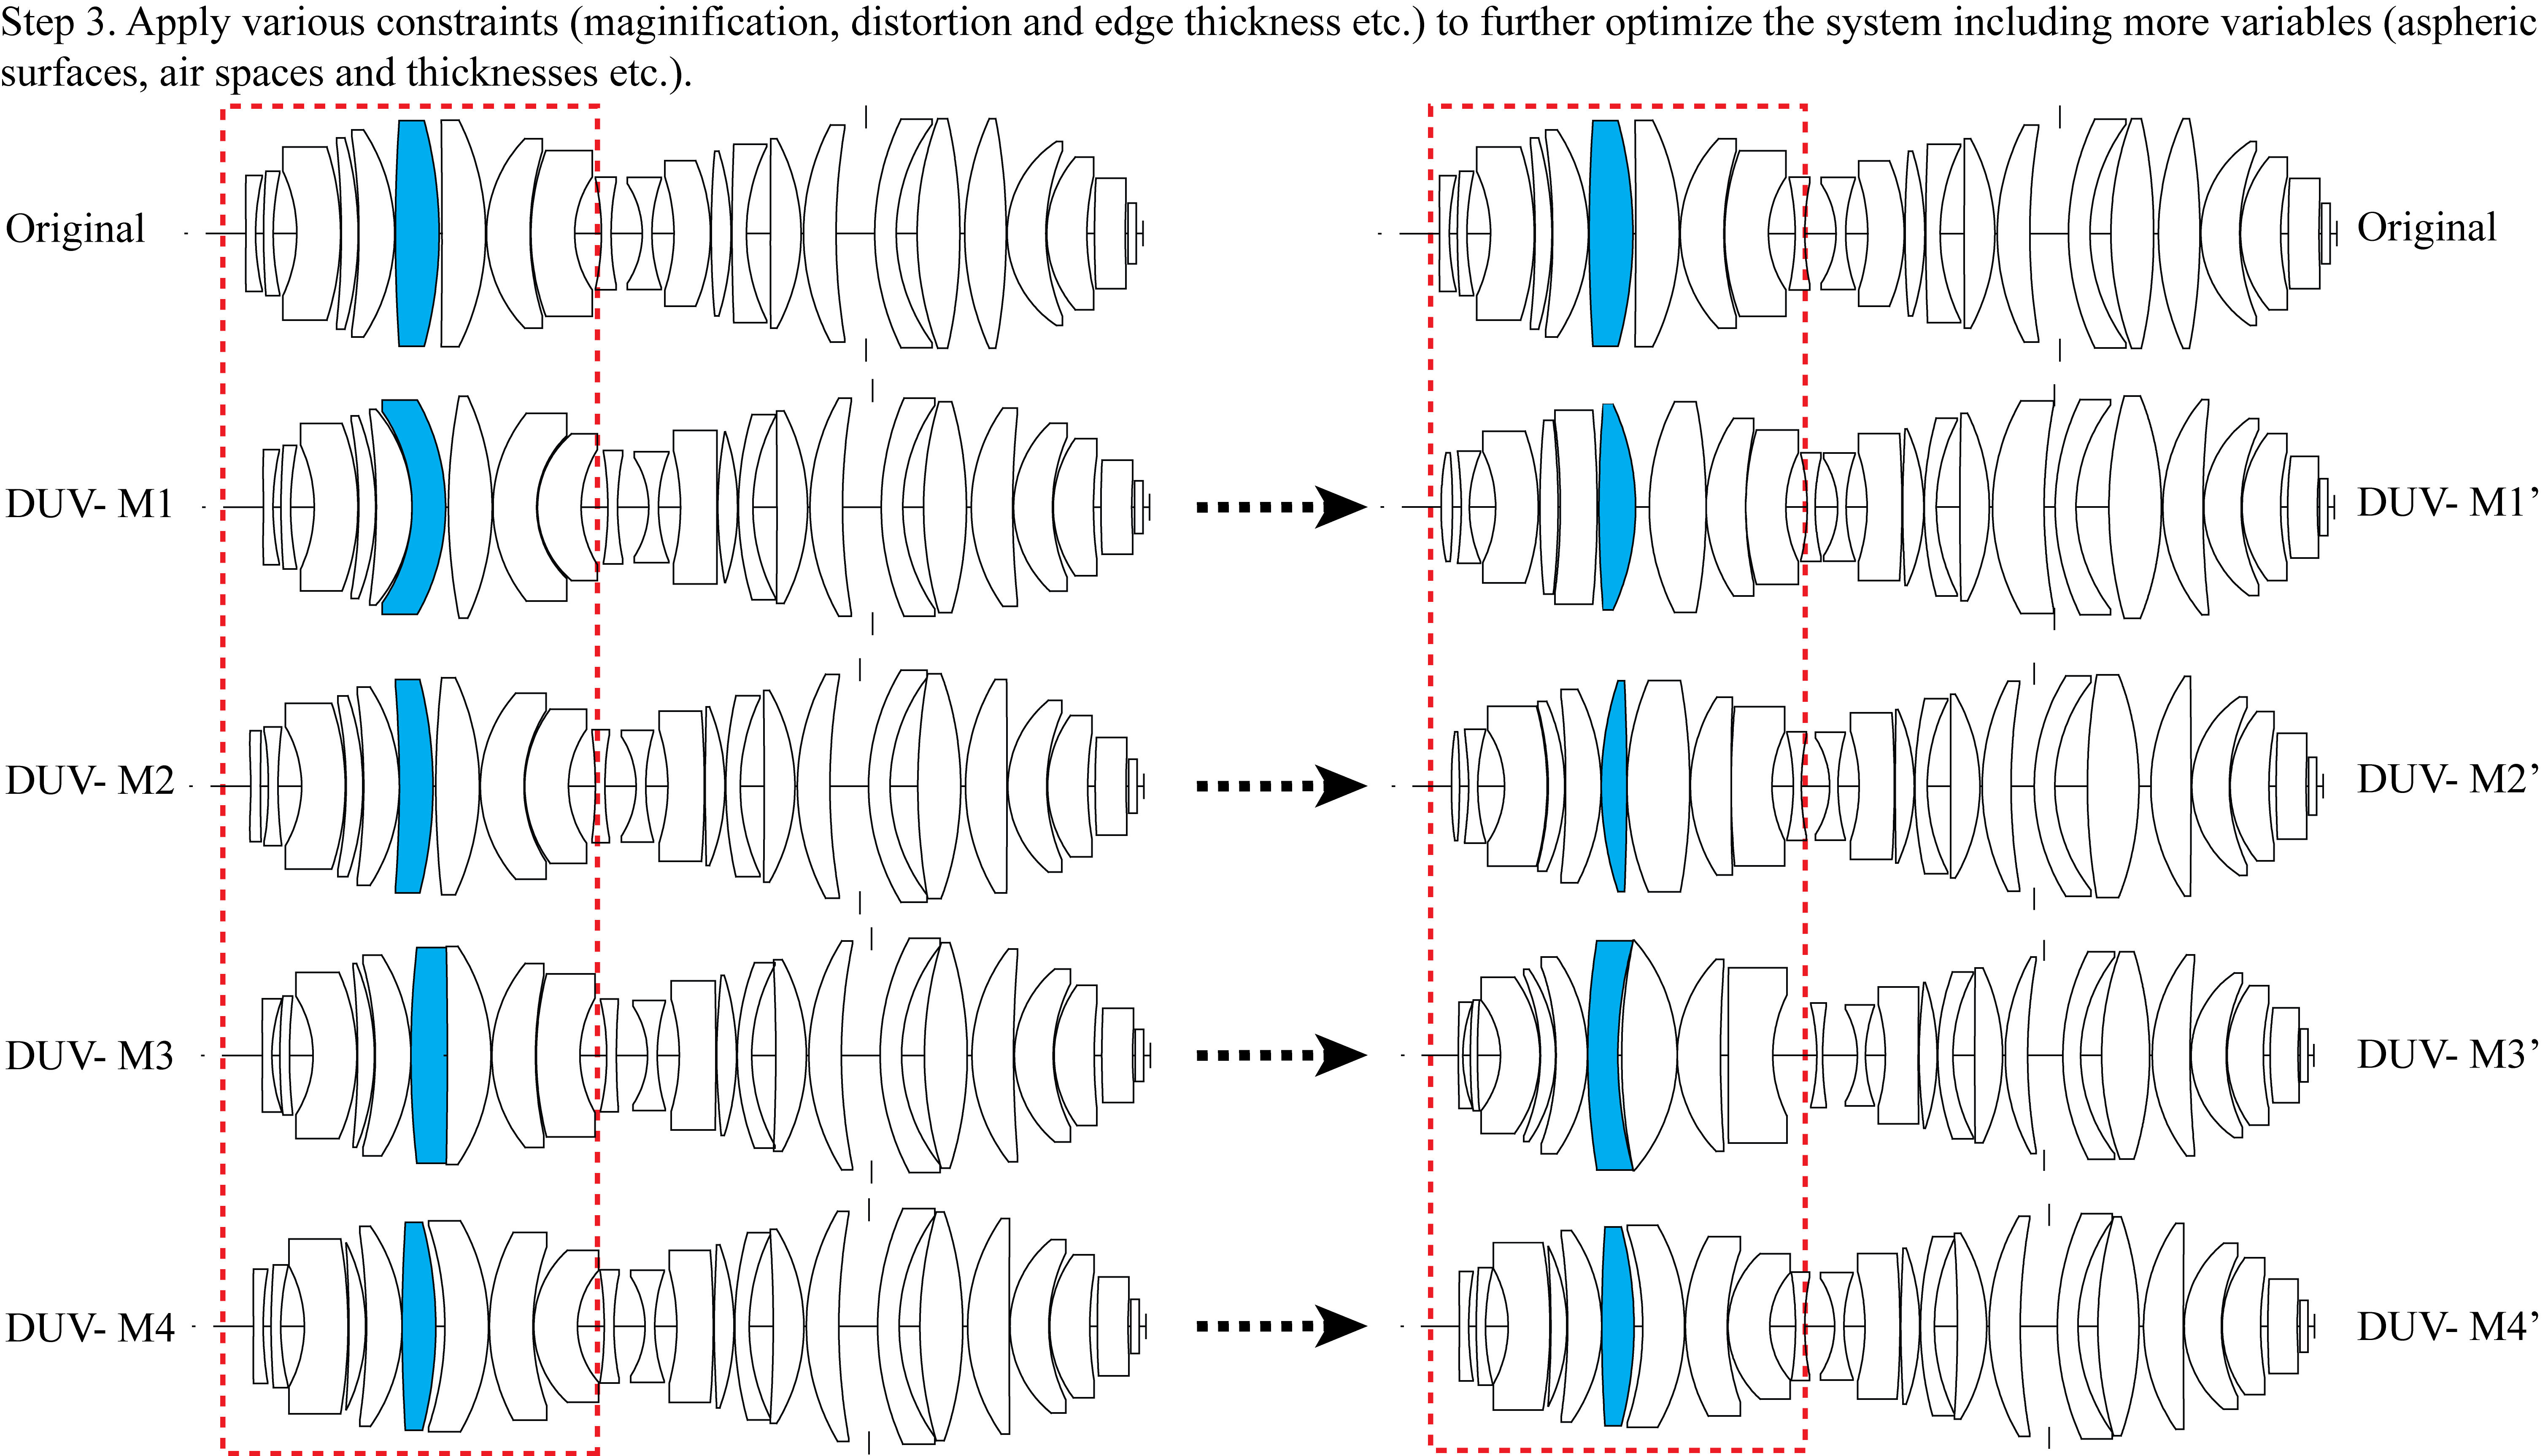
\includegraphics[width=\textwidth]{chapter-4/figures/Litho_SPC_minima_listed.png}
    \caption{Step 3 of performing SPC on a lithographic objective: applying constraints to the systems obtained from the SPC and further optimize the systems using more variables (thickness, aspheric terms, etc.). The optimized systems are evaluated on their performances.}
    \label{fig: litho_Step3}
\end{figure}

In Table \ref{table: Litho_final_solution}, the performances of the four optimized solutions are listed. While minimizing the wavefront aberration (in RMS), the distortion and the telecentricity are controlled at the same time. Among the four new solutions, DUV-M3' shows better wavefront RMS (29$\%$ better than the orignal), distortion (16\text{\%}), and telecentricity at the image side (94$\%$). The telecentricity at the object side is worse than the original one (15$\%$). The other three new solutions show some mixed performances, with some properties better than the original system, but others worse. For a practical case, more properties have to be considered in designing a lithographic system, e.g. thermal sensitivity, manufacturability and cost. In our example, the assessing criteria have been limited to those mentioned above. The results show that with SPC and the design flow used, new solutions in a complex lithographic system can be systematically found. In the example discussed, systems with better and worse performance as compared to the original, are obtained. 

\setlength{\arrayrulewidth}{.5mm}
\setlength{\tabcolsep}{18pt}
\renewcommand{\arraystretch}{1.2}
\begin{table}[h!]
    \centering
    \captionsetup{justification=centering}
    \caption{Performance of the optimized solutions shown in Figure \ref{fig: litho_Step3}}
    \label{table: Litho_final_solution}
    \vspace{-1em}
    % \hspace*{-10pt} %adjusting the position of the plot(table) !!!!
    \begin{adjustbox}{max width=\textwidth, center}
    \begin{tabular}{c c c c c}
    \hline 
       & \textbf{Wavefront RMS (m\textlambda)} & \textbf{Distortion (nm)} & \textbf{Object Side Telecentricity* (mrad)} & \textbf{Image Side Telecentricity* (mrad)} \\ 
     \midrule
    Original & 3.26 & <1.00 & <14.36 & <19.18 \\ 
    \midrule
    DUV-M1' & 2.96 & <1.62 & <17.60 & <17.31 \\ 
    \midrule
    DUV-M2' & 3.36 & <1.43 & <17.98 & <5.84 \\ 
    \midrule
    DUV-M3' & 2.32 & <0.84 & <16.56 & <1.15 \\ 
    \midrule
    DUV-M4' & 9.91 & <2.39 & <57.01 & <10.05\\
    \hline
    \small* 'Telecentricity' here means the deviation from telecentricity.
    \end{tabular}
    \end{adjustbox}
\end{table}


\section{Conclusion}
In this chapter, multiple examples are given to demonstrate how SPC can be applied in practical lens designs. It is recommended to integrate the SPC method with conventional strategies. In this way, more solutions can be effectively produced and from them the designer should then choose the best. In the example of a wide-angle lens, where the system is divided into two groups, we show that SPC can be applied to the individual group of lenses or to the wide-angle lens combined from the two groups of lenses. Applying SPC in this wide-angle lens design helps to produce alternative solutions in the landscape. For complex system like the UV microscope objective, guided by the designer's knowledge, SPC shows better efficiency than the conventional approaches in terms of obtaining good solutions. In order to design a lithographic objective with multiple constraints, it is discussed how SPC can be integrated in a two-step design process. New solutions with local changes are obtained with mixed performances in the sense that the obtained systems, compared to the original system, are better in some aspects and worse in others. 

With the wide-angle lens, detailed steps for applying the SPC to switch to new solutions are given. The basin plots in Figure \ref{fig:basins} reveal that in some cases the obtained minima depend on the choice of the optimization starting point around the saddle point. This dependency can be a property of the design landscape, or it can be caused by the numerical configuration (e.g. choices of the damping factor) of the local optimizer. Further research is necessary to understand this phenomenon. For the given example, this dependency between the starting point and the local minima with zero-thickness element did not influence the final results after increasing the thickness for the zero-thickness minima (Table \ref{table: scanline}).

Factors that will alter the SPC scan curve are investigated. These factors are: 1) When the number of variables increases (fourteen for the UV microscope objective), a shallow local minimum should be very well optimized to ensure that the correct SPC scan curve is obtained; 2) When constraint type and weights are varied, the corresponding SPC scan curves are different. We observe that more constraints and more rigid weights (leading to a stressed system) result in fewer saddle points than fewer constraints and more flexible weights (which leads to a relaxed system). Therefore, it is recommended to implement only the necessary constraints at the SPC scan stage. Extreme values of these constraints should also be avoided. It is better to add the other constraint later in the design process.

In conclusion, to design a complex system, applying SPC following the guidelines presented in this chapter will help to generate (intermediate) solutions effectively. When implementing the SPC method in a software package to serve as a lens optimization tool, the cases discussed in this chapter should be taken into account (e.g. automatically verify the SPC scan curve stability) to assist the design process.  


\references{dissertation}

